% Options for packages loaded elsewhere
\PassOptionsToPackage{unicode}{hyperref}
\PassOptionsToPackage{hyphens}{url}
\PassOptionsToPackage{dvipsnames,svgnames,x11names}{xcolor}
%
\documentclass[
  letterpaper,
  DIV=11,
  numbers=noendperiod]{scrreprt}

\usepackage{amsmath,amssymb}
\usepackage{lmodern}
\usepackage{iftex}
\ifPDFTeX
  \usepackage[T1]{fontenc}
  \usepackage[utf8]{inputenc}
  \usepackage{textcomp} % provide euro and other symbols
\else % if luatex or xetex
  \usepackage{unicode-math}
  \defaultfontfeatures{Scale=MatchLowercase}
  \defaultfontfeatures[\rmfamily]{Ligatures=TeX,Scale=1}
  \setmainfont[]{Noto Sans}
\fi
% Use upquote if available, for straight quotes in verbatim environments
\IfFileExists{upquote.sty}{\usepackage{upquote}}{}
\IfFileExists{microtype.sty}{% use microtype if available
  \usepackage[]{microtype}
  \UseMicrotypeSet[protrusion]{basicmath} % disable protrusion for tt fonts
}{}
\makeatletter
\@ifundefined{KOMAClassName}{% if non-KOMA class
  \IfFileExists{parskip.sty}{%
    \usepackage{parskip}
  }{% else
    \setlength{\parindent}{0pt}
    \setlength{\parskip}{6pt plus 2pt minus 1pt}}
}{% if KOMA class
  \KOMAoptions{parskip=half}}
\makeatother
\usepackage{xcolor}
\setlength{\emergencystretch}{3em} % prevent overfull lines
\setcounter{secnumdepth}{5}
% Make \paragraph and \subparagraph free-standing
\ifx\paragraph\undefined\else
  \let\oldparagraph\paragraph
  \renewcommand{\paragraph}[1]{\oldparagraph{#1}\mbox{}}
\fi
\ifx\subparagraph\undefined\else
  \let\oldsubparagraph\subparagraph
  \renewcommand{\subparagraph}[1]{\oldsubparagraph{#1}\mbox{}}
\fi


\providecommand{\tightlist}{%
  \setlength{\itemsep}{0pt}\setlength{\parskip}{0pt}}\usepackage{longtable,booktabs,array}
\usepackage{calc} % for calculating minipage widths
% Correct order of tables after \paragraph or \subparagraph
\usepackage{etoolbox}
\makeatletter
\patchcmd\longtable{\par}{\if@noskipsec\mbox{}\fi\par}{}{}
\makeatother
% Allow footnotes in longtable head/foot
\IfFileExists{footnotehyper.sty}{\usepackage{footnotehyper}}{\usepackage{footnote}}
\makesavenoteenv{longtable}
\usepackage{graphicx}
\makeatletter
\def\maxwidth{\ifdim\Gin@nat@width>\linewidth\linewidth\else\Gin@nat@width\fi}
\def\maxheight{\ifdim\Gin@nat@height>\textheight\textheight\else\Gin@nat@height\fi}
\makeatother
% Scale images if necessary, so that they will not overflow the page
% margins by default, and it is still possible to overwrite the defaults
% using explicit options in \includegraphics[width, height, ...]{}
\setkeys{Gin}{width=\maxwidth,height=\maxheight,keepaspectratio}
% Set default figure placement to htbp
\makeatletter
\def\fps@figure{htbp}
\makeatother

\usepackage{booktabs}
\usepackage{longtable}
\usepackage{array}
\usepackage{multirow}
\usepackage{wrapfig}
\usepackage{float}
\usepackage{colortbl}
\usepackage{pdflscape}
\usepackage{tabu}
\usepackage{threeparttable}
\usepackage{threeparttablex}
\usepackage[normalem]{ulem}
\usepackage{makecell}
\usepackage{xcolor}
\KOMAoption{captions}{tableheading}
\makeatletter
\@ifpackageloaded{tcolorbox}{}{\usepackage[many]{tcolorbox}}
\@ifpackageloaded{fontawesome5}{}{\usepackage{fontawesome5}}
\definecolor{quarto-callout-color}{HTML}{909090}
\definecolor{quarto-callout-note-color}{HTML}{0758E5}
\definecolor{quarto-callout-important-color}{HTML}{CC1914}
\definecolor{quarto-callout-warning-color}{HTML}{EB9113}
\definecolor{quarto-callout-tip-color}{HTML}{00A047}
\definecolor{quarto-callout-caution-color}{HTML}{FC5300}
\definecolor{quarto-callout-color-frame}{HTML}{acacac}
\definecolor{quarto-callout-note-color-frame}{HTML}{4582ec}
\definecolor{quarto-callout-important-color-frame}{HTML}{d9534f}
\definecolor{quarto-callout-warning-color-frame}{HTML}{f0ad4e}
\definecolor{quarto-callout-tip-color-frame}{HTML}{02b875}
\definecolor{quarto-callout-caution-color-frame}{HTML}{fd7e14}
\makeatother
\makeatletter
\makeatother
\makeatletter
\@ifpackageloaded{bookmark}{}{\usepackage{bookmark}}
\makeatother
\makeatletter
\@ifpackageloaded{caption}{}{\usepackage{caption}}
\AtBeginDocument{%
\ifdefined\contentsname
  \renewcommand*\contentsname{Table of contents}
\else
  \newcommand\contentsname{Table of contents}
\fi
\ifdefined\listfigurename
  \renewcommand*\listfigurename{List of Figures}
\else
  \newcommand\listfigurename{List of Figures}
\fi
\ifdefined\listtablename
  \renewcommand*\listtablename{List of Tables}
\else
  \newcommand\listtablename{List of Tables}
\fi
\ifdefined\figurename
  \renewcommand*\figurename{Figure}
\else
  \newcommand\figurename{Figure}
\fi
\ifdefined\tablename
  \renewcommand*\tablename{Table}
\else
  \newcommand\tablename{Table}
\fi
}
\@ifpackageloaded{float}{}{\usepackage{float}}
\floatstyle{ruled}
\@ifundefined{c@chapter}{\newfloat{codelisting}{h}{lop}}{\newfloat{codelisting}{h}{lop}[chapter]}
\floatname{codelisting}{Listing}
\newcommand*\listoflistings{\listof{codelisting}{List of Listings}}
\makeatother
\makeatletter
\@ifpackageloaded{caption}{}{\usepackage{caption}}
\@ifpackageloaded{subcaption}{}{\usepackage{subcaption}}
\makeatother
\makeatletter
\@ifpackageloaded{tcolorbox}{}{\usepackage[many]{tcolorbox}}
\makeatother
\makeatletter
\@ifundefined{shadecolor}{\definecolor{shadecolor}{rgb}{.97, .97, .97}}
\makeatother
\makeatletter
\makeatother
\ifLuaTeX
  \usepackage{selnolig}  % disable illegal ligatures
\fi
\IfFileExists{bookmark.sty}{\usepackage{bookmark}}{\usepackage{hyperref}}
\IfFileExists{xurl.sty}{\usepackage{xurl}}{} % add URL line breaks if available
\urlstyle{same} % disable monospaced font for URLs
\hypersetup{
  pdftitle={Richmond Regional Housing Framework Data Update},
  pdfauthor={HDAdvisors},
  colorlinks=true,
  linkcolor={blue},
  filecolor={Maroon},
  citecolor={Blue},
  urlcolor={Blue},
  pdfcreator={LaTeX via pandoc}}

\title{Richmond Regional Housing Framework Data Update}
\author{HDAdvisors}
\date{1/4/23}

\begin{document}
\maketitle
\ifdefined\Shaded\renewenvironment{Shaded}{\begin{tcolorbox}[borderline west={3pt}{0pt}{shadecolor}, breakable, enhanced, interior hidden, sharp corners, frame hidden, boxrule=0pt]}{\end{tcolorbox}}\fi

\renewcommand*\contentsname{Table of contents}
{
\hypersetup{linkcolor=}
\setcounter{tocdepth}{2}
\tableofcontents
}
\bookmarksetup{startatroot}

\hypertarget{about}{%
\chapter*{About}\label{about}}
\addcontentsline{toc}{chapter}{About}

\markboth{About}{About}

This report is a data update for the Richmond Regional Housing
Framework, which was
\href{https://pharva.com/framework/about-the-framework/}{released} by
the Partnership for Housing Affordability (PHA) in January 2020. It will
support PHA's ongoing efforts to educate both decision-makers and the
public at large about the region's housing needs and opportunities. Data
in the report will also help PHA continue to monitor, change, and
implement the policy solutions outlined in the Framework.

There are four parts in this report:

\begin{enumerate}
\def\labelenumi{\arabic{enumi}.}
\tightlist
\item
  Demographic and socioeconomic changes
\item
  Housing supply and market changes
\item
  Gap analysis
\item
  Local summaries
\end{enumerate}

\part{PART 1: Demographic and socioeconomic changes}

\hypertarget{part-1-1}{%
\chapter{Population changes}\label{part-1-1}}

This chapter covers population changes across the Partnership for
Housing Affordability's main coverage area, including the City of
Richmond and the counties of Chesterfield, Hanover, and Henrico.

\hypertarget{total-population-growth}{%
\section{Total population growth}\label{total-population-growth}}

The Richmond region has continued to grow between 2016 and 2020---adding
a net of 41,457 residents across the four major localities. The most
populous locality, Chesterfield County, experienced a near eight percent
increase in its population during this timeframe.

\begin{figure}

{\centering 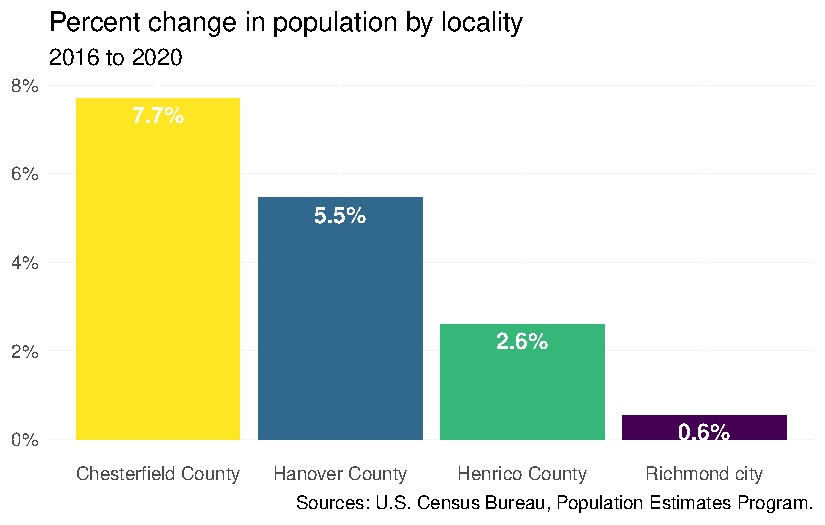
\includegraphics{./part-1-1_files/figure-pdf/fig-total-pop-plot-1.pdf}

}

\caption{\label{fig-total-pop-plot}Percent change in population by
locality}

\end{figure}

\hypertarget{components-of-population-change}{%
\section{Components of population
change}\label{components-of-population-change}}

In recent years, nearly two thirds of growth could be attributed to
either domestic or international migration into the region. But between
2020 and 2021, that share increased to over three quarters---reducing
the portion of the population growing due to natural increase to only 13
percent.

The region's growth continues to be driven primarily by new people
coming from other parts of the state and nation (64 percent of growth
between 2020 and 2021).

\begin{figure}

{\centering 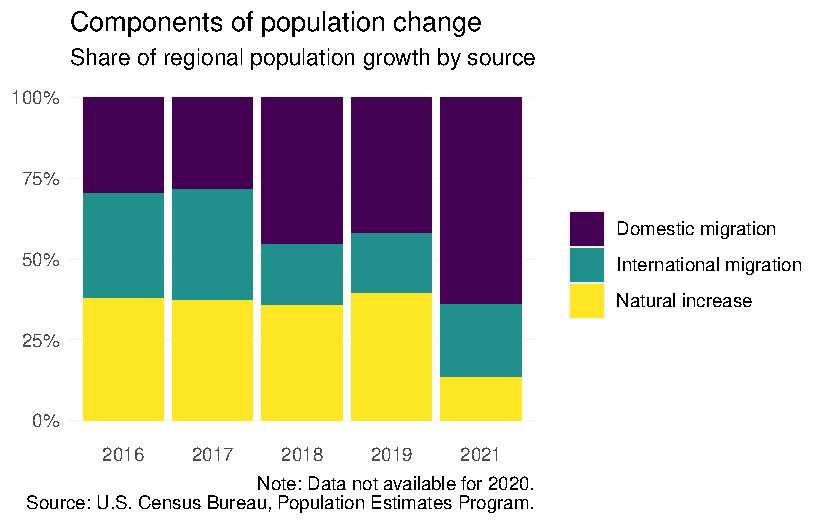
\includegraphics{./part-1-1_files/figure-pdf/fig-components-plot-1.pdf}

}

\caption{\label{fig-components-plot}Components of population change}

\end{figure}

\hypertarget{population-projections}{%
\section{Population projections}\label{population-projections}}

Between 2020 and 2050, the region is expected to grow by nearly a third
(29 percent)---reaching 1,338,306 residents.

\begin{figure}

{\centering 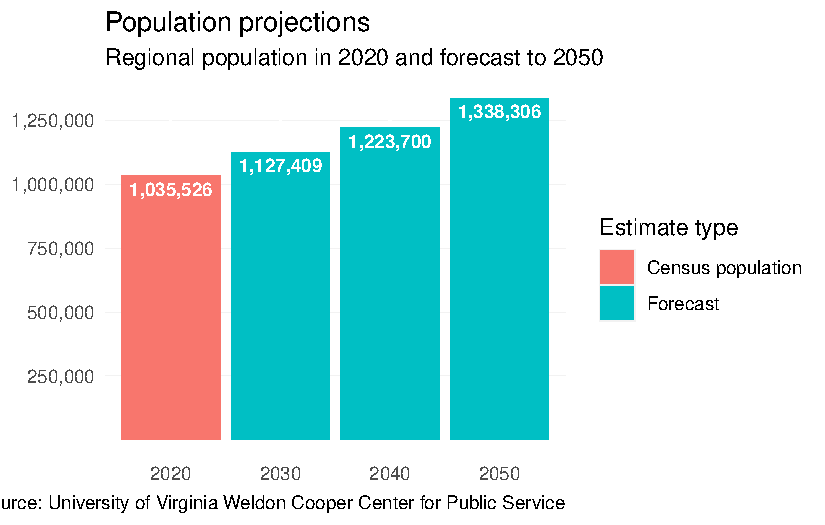
\includegraphics{./part-1-1_files/figure-pdf/fig-forecasts-region-plot-1.pdf}

}

\caption{\label{fig-forecasts-region-plot}Population projections}

\end{figure}

Over the next 30 years, Chesterfield County will continue to lead growth
across the region. By 2050, Chesterfield is expected to surpass half a
million residents, growing by 38 percent from the 2020 Census estimates.

Population growth trends will largely continue as they have with Hanover
County experiencing the second greatest growth from their 2020 estimates
(27 percent increase). Henrico County follows with a 26 percent increase
(+88,565), while the City of Richmond will only increase by about a
fifth (20 percent) over 30 years.

\begin{figure}

{\centering 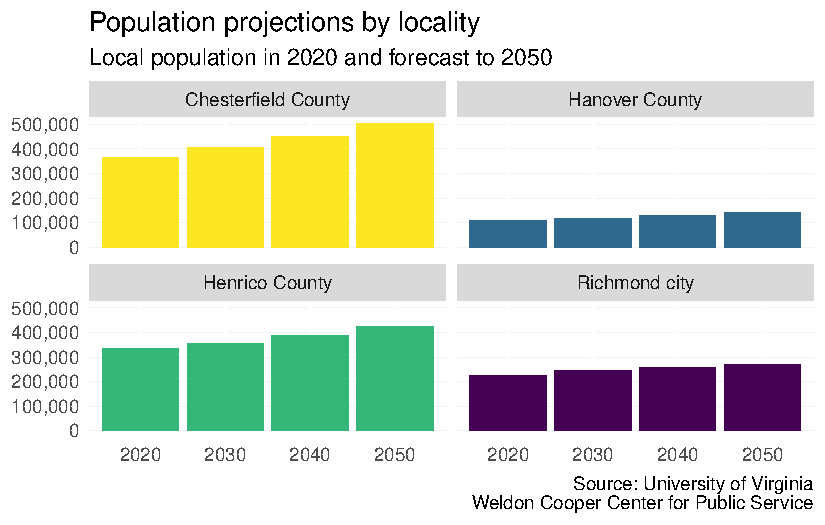
\includegraphics{./part-1-1_files/figure-pdf/fig-forecasts-locality-plot-1.pdf}

}

\caption{\label{fig-forecasts-locality-plot}Population projections by
locality}

\end{figure}

\hypertarget{part-1-2}{%
\chapter{Household characteristics}\label{part-1-2}}

This chapter covers the household trends that influence housing demand
across the Partnership for Housing Affordability's coverage area,
including, but not limited to householder age, household size, and
multigenerational households.

\hypertarget{household-formation}{%
\section{Household formation}\label{household-formation}}

According to Census estimates, the region gained more than 15,000
households from 2016 to 2020. This growth was driven entirely by new
homeowners (17,436). Renter households, instead, saw much slower
increases from 2016 to 2019; from 2019 to 2020, the estimated number of
renters dropped more than 2,000 for a net loss of 609 over the full
period.

\begin{tcolorbox}[enhanced jigsaw, colframe=quarto-callout-warning-color-frame, arc=.35mm, bottomrule=.15mm, colbacktitle=quarto-callout-warning-color!10!white, opacityback=0, left=2mm, rightrule=.15mm, title=\textcolor{quarto-callout-warning-color}{\faExclamationTriangle}\hspace{0.5em}{Pandemic impacts on data reliability}, colback=white, coltitle=black, toptitle=1mm, leftrule=.75mm, titlerule=0mm, breakable, opacitybacktitle=0.6, toprule=.15mm, bottomtitle=1mm]

This anomalous data should be treated with caution. Lower American
Community Survey response rates during COVID-19 were most common among
lower-income and lower-educated households most likely to rent. Across
the Richmond region, overall ACS response rates
\href{https://www.prb.org/articles/capturing-covids-impact-on-the-american-community-survey-across-counties/}{declined
nearly 10 percent} from the 2015-2019 to 2016-2020 collection period.

\end{tcolorbox}

\begin{figure}

{\centering 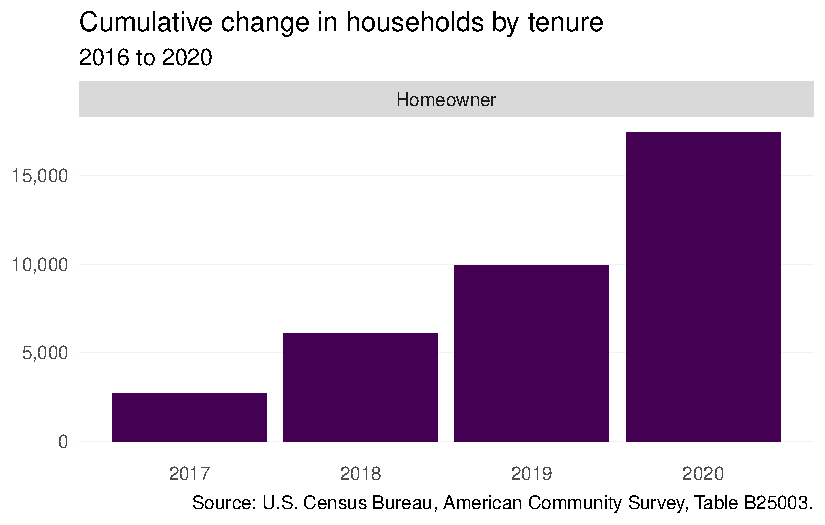
\includegraphics{./part-1-2_files/figure-pdf/fig-hh-form-plot-1.pdf}

}

\caption{\label{fig-hh-form-plot}Cumulative change in households by
tenure}

\end{figure}

\hypertarget{households-by-age}{%
\section{Households by age}\label{households-by-age}}

The single largest growing cohort of households across the region are
homeowners 65 years and over. Thanks in large part to youngest baby
boomers aging into retirement, this group increased by more than 13,000.
Younger homeowners saw much smaller gains.

Among renters, most growth occurred in senior householders. The
significant decrease of renter households under 25 (more than 3,200)
should be treated with caution, as this population likely had much lower
ACS response rates during COVID-19.

\begin{figure}

{\centering 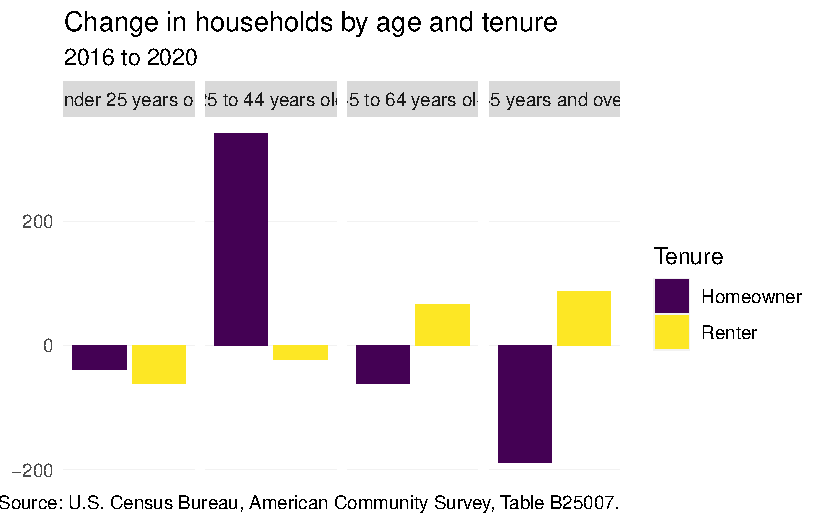
\includegraphics{./part-1-2_files/figure-pdf/fig-hh-age-plot-1.pdf}

}

\caption{\label{fig-hh-age-plot}Change in households by age and tenure}

\end{figure}

\hypertarget{households-by-type}{%
\section{Households by type}\label{households-by-type}}

Married-couple families continued to be the dominant household type in
the region, growing by 9,625 from 2016 to 2020. Living alone also become
more common, likely the result of seniors increasingly living on their
own. Households headed by single females were the only type to decline;
however, this could potentially be attributed to lower ACS response
rates among those households during COVID-19.

\begin{figure}

{\centering 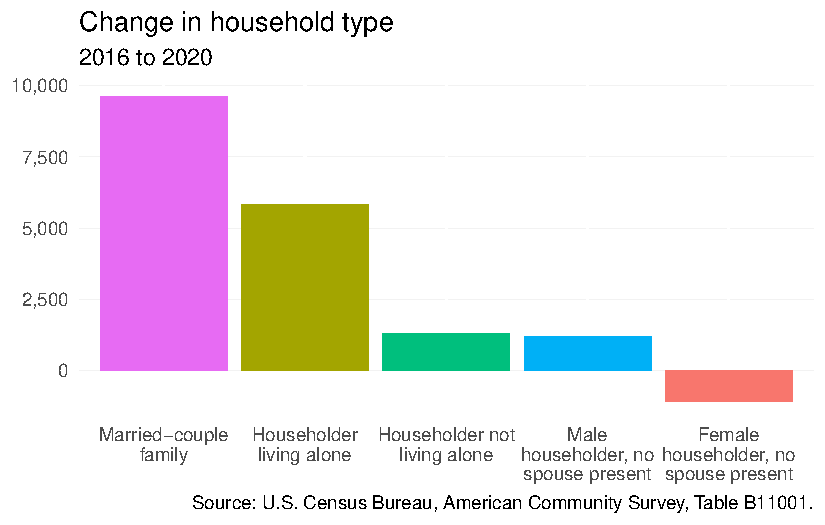
\includegraphics{./part-1-2_files/figure-pdf/fig-hh-type-plot-1.pdf}

}

\caption{\label{fig-hh-type-plot}Change in household type}

\end{figure}

\hypertarget{households-by-size}{%
\section{Households by size}\label{households-by-size}}

Two-person homeowning households were by and large the fastest-growing
cohort among different size households from 2016 to 2020. There was also
a significant increase in the number of homeowners living alone, as well
as homeowners with four-person households.

Persons living alone were the only size of renter households that grew
with any significance over this period. One potential explanation for
the notable decreases in the number of three- and four-person renter
households is lower ACS response rates among younger adults living with
roommates during COVID-19. This population, which does not include
college students living in dorms (``group quarters'' are not households
in Census methodology), was likely to move back home with parents during
the initial phases of the pandemic.

\begin{figure}

{\centering 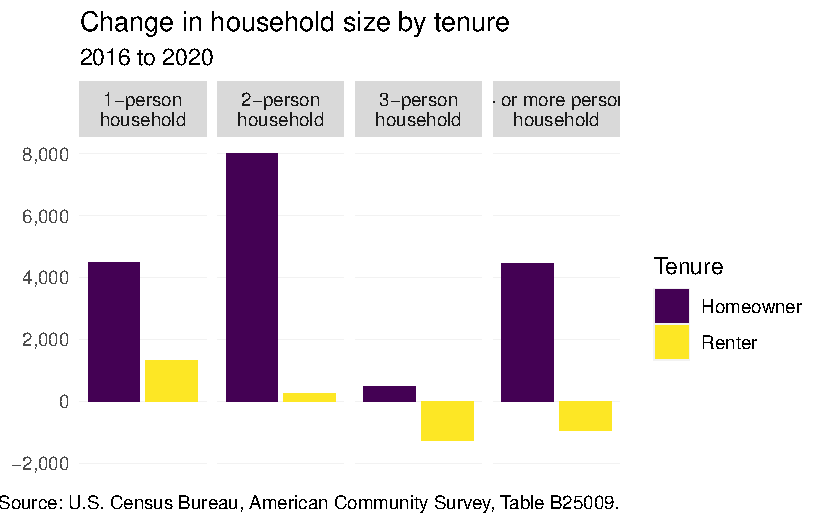
\includegraphics{./part-1-2_files/figure-pdf/fig-hh-size-plot-1.pdf}

}

\caption{\label{fig-hh-size-plot}Change in household size by tenure}

\end{figure}

\hypertarget{households-with-children}{%
\section{Households with children}\label{households-with-children}}

The number of homeowners without children in the region grew
significantly (by almost 9,000) from 2016 to 2020. This is likely due in
large part to baby boomer parents now living without their children. The
number of homeowners in nonfamily households also increased---driven
primarily by those now living alone. Families with children were the
least common group of homeowners that grew.

The only group of renters that saw significant growth was nonfamily
households. This includes both renters that live alone and those that
live with non-related roommates. The estimated number of renters with
children declined sharply; this may also be a symptom of lower pandemic
ACS responses among lower-income working families.

\begin{figure}

{\centering 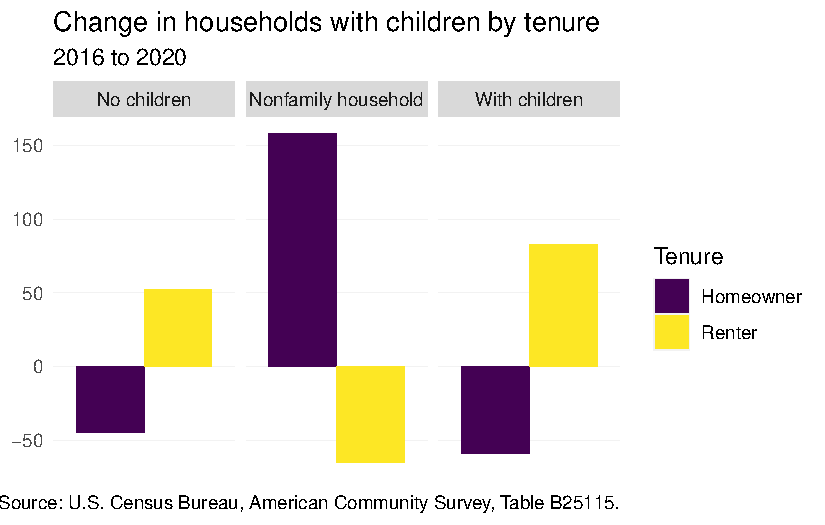
\includegraphics{./part-1-2_files/figure-pdf/fig-hh-child-plot-1.pdf}

}

\caption{\label{fig-hh-child-plot}Change in households with children by
tenure}

\end{figure}

\hypertarget{senior-living-arrangements}{%
\section{Senior living arrangements}\label{senior-living-arrangements}}

Since 2016, the region's senior population increased almost exclusively
among three types:

\begin{itemize}
\tightlist
\item
  Seniors who are the head of the household,
\item
  Seniors who are the spouse of the head of the households, and
\item
  Seniors who live alone.
\end{itemize}

The estimated number of seniors within group quarters (e.g.~nursing
homes, assisted living facilities) increased by less than 200. This
figure should be assessed in context of ACS collection
\href{https://www.census.gov/newsroom/blogs/random-samplings/2021/09/collecting-acs-data-from-group-quarters-amid-the-pandemic.html}{challenges}
in group quarters settings throughout the COVID-19 pandemic.

\begin{figure}

{\centering 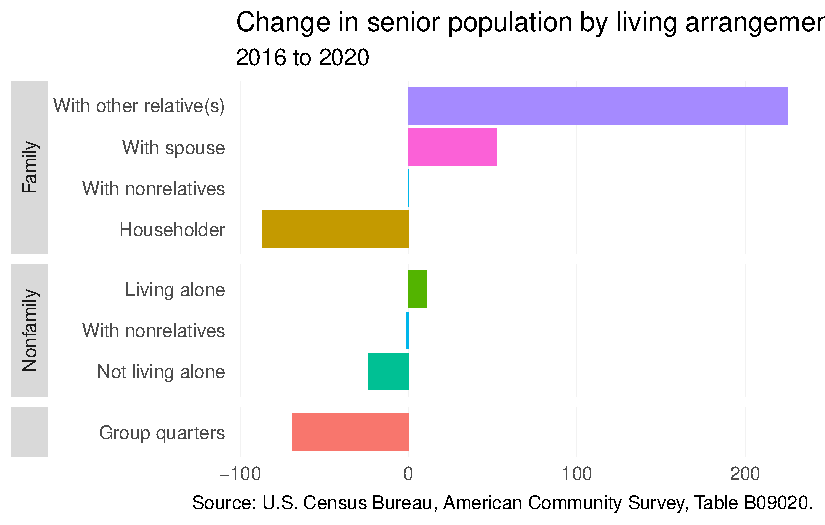
\includegraphics{./part-1-2_files/figure-pdf/fig-hh-seniors-plot-1.pdf}

}

\caption{\label{fig-hh-seniors-plot}Change in senior population by
living arrangement}

\end{figure}

\hypertarget{subfamilies}{%
\section{Subfamilies}\label{subfamilies}}

The Census Bureau defines a \emph{subfamily} as a group of related
individuals who live in the household of someone else. As of 2020, there
were approximately 9,850 subfamilies across the region. Two-thirds of
those are single mothers living with at least one child of their own.
These estimates have remained stable since 2016.

\begin{figure}

{\centering 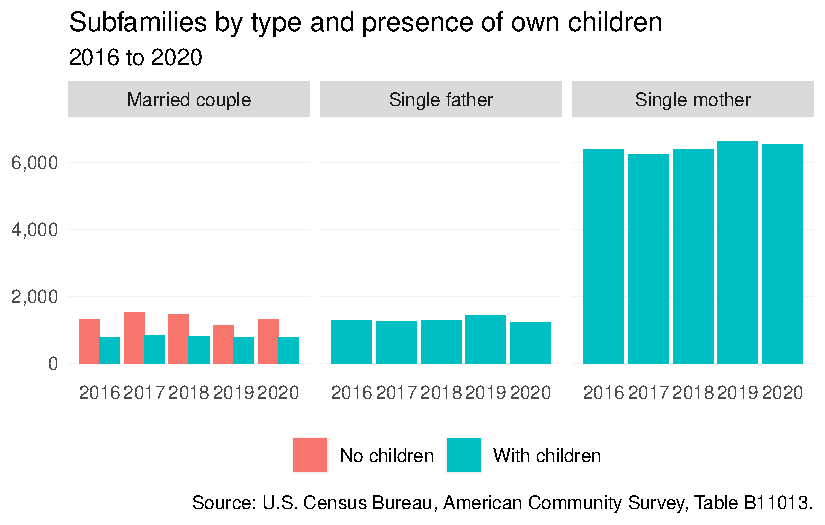
\includegraphics{./part-1-2_files/figure-pdf/fig-hh-subfam-plot-1.pdf}

}

\caption{\label{fig-hh-subfam-plot}Subfamilies by type and presence of
own children}

\end{figure}

\hypertarget{multigenerational-households}{%
\section{Multigenerational
households}\label{multigenerational-households}}

The Census Bureau defines \emph{multigenerational} households as those
with three or more generations. According to the Pew Research Center,
the share of the American population in multigenerational households
\href{https://www.pewresearch.org/social-trends/2022/03/24/the-demographics-of-multigenerational-households/}{increased}
from just 7 percent in 1971 to 18 percent in 2021.

However, multigenerational households in the Richmond region are less
common than the national average. As of 2020, the share of persons in
multiple generation households across the region has stayed between 7
and 8 percent from 2016 to 2020.

\begin{tcolorbox}[enhanced jigsaw, colframe=quarto-callout-note-color-frame, arc=.35mm, bottomrule=.15mm, colbacktitle=quarto-callout-note-color!10!white, opacityback=0, left=2mm, rightrule=.15mm, title=\textcolor{quarto-callout-note-color}{\faInfo}\hspace{0.5em}{Note}, colback=white, coltitle=black, toptitle=1mm, leftrule=.75mm, titlerule=0mm, breakable, opacitybacktitle=0.6, toprule=.15mm, bottomtitle=1mm]

Multigenerational households estimates are not available from the
standard ACS tables published by the Census Bureau. The data in this
section comes from the Public Use Microdata Sample (PUMS), which are
available only by special Public Use Microdata Areas (PUMAs) which
contain at least 100,000 people.

While PUMA boundaries align with Chesterfield County, Henrico County,
and Richmond city, the PUMA containing Hanover County also includes
Powhatan, Goochland, New Kent, King William, Charles City counties.

\end{tcolorbox}

Multigenerational households are slightly more common in the core metro
area (Chesterfield, Henrico, and Richmond) than the outlying suburbs.
The share of multigenerational households in Chesterfield and Richmond
appears to be decreasing slightly, while increasing slightly in the
outer counties. The share of Henrico's population in multigenerational
households continues to sit around 8 percent.

\begin{figure}

{\centering 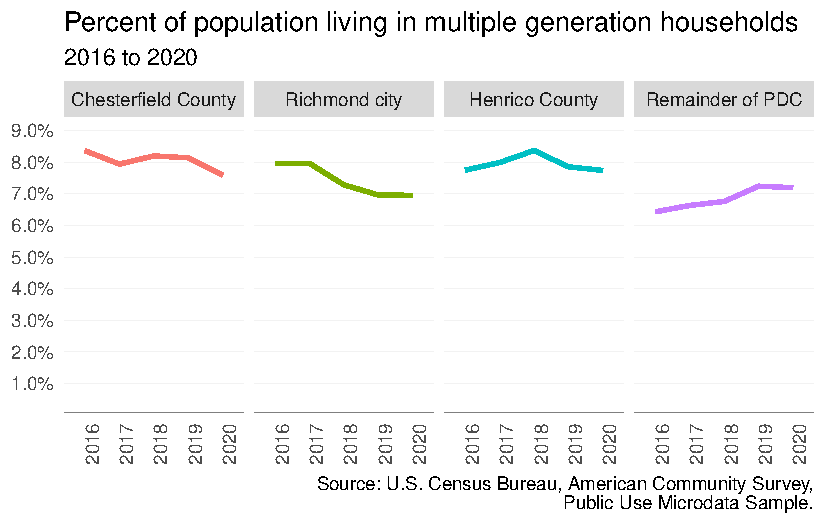
\includegraphics{./part-1-2_files/figure-pdf/fig-hh-multigen-plot-1.pdf}

}

\caption{\label{fig-hh-multigen-plot}Percent of population living in
multiple generation households}

\end{figure}

\hypertarget{adult-children-with-parents}{%
\section{Adult children with
parents}\label{adult-children-with-parents}}

Over the past decade, a common stereotype has been that of adult
millennial child continuing to live with their parents. While this trope
is based in real economic challenges faced by young adults, such as
increasing housing costs and student debt, its magnitude can often be
overstated.

Today, more than 75,800 adults 18 to 34 years old in the region---about
one-in-three---live with their parents. This is more than any other
arrangement. However, since 2016, the fastest growing living arrangement
for young adults has been with an unmarried partner, followed by other
nonrelatives (roommates). In fact, the share of young adults now living
with a married spouse increased slightly more than the share still
living with parents.

\begin{figure}

{\centering 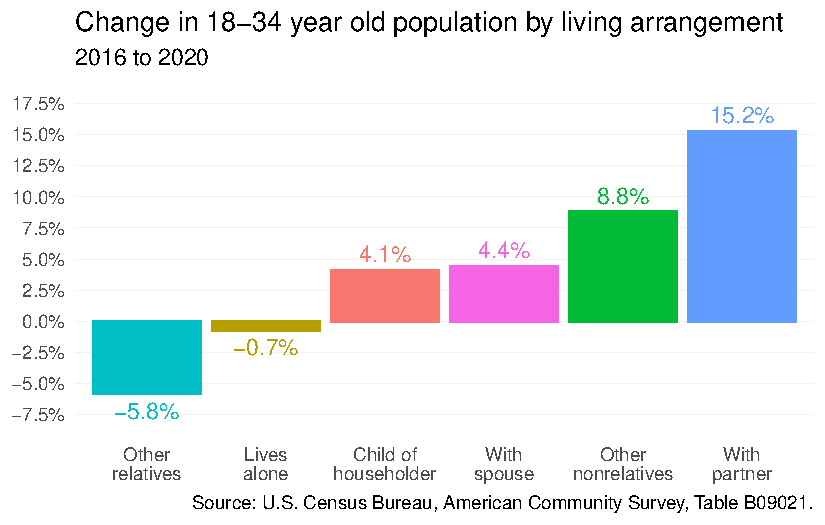
\includegraphics{./part-1-2_files/figure-pdf/fig-hh-adultchild-plot-1.pdf}

}

\caption{\label{fig-hh-adultchild-plot}Change in 18-34 year old
population by living arrangement}

\end{figure}

\hypertarget{part-1-3}{%
\chapter{Incomes and wages}\label{part-1-3}}

This chapter covers the changes in incomes and wages among households
and occupations across the region.

\hypertarget{household-incomes}{%
\section{Household incomes}\label{household-incomes}}

\hypertarget{incomes-by-tenure}{%
\subsection{Incomes by tenure}\label{incomes-by-tenure}}

From 2016 to 2020, the region saw large increases in the number of
six-figure income households, particularly among homeowners (well over
25,000), but also renters (almost 6,500). This growth can likely be
attributed to both new high-income residents from outside the region, as
well as income growth among households already in the region.

There was also a minor increase in the number of middle-income renters
earning between \$50,000 and \$100,000, reflecting continued demand for
new market-rate apartments---along with affordable starter homes.

\begin{figure}

{\centering 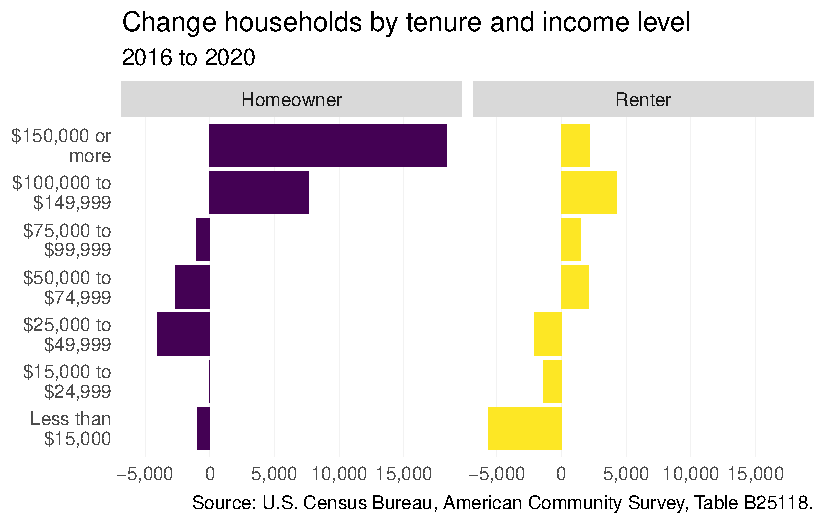
\includegraphics{./part-1-3_files/figure-pdf/fig-hh-inc-plot-1.pdf}

}

\caption{\label{fig-hh-inc-plot}Change households by tenure and income
level}

\end{figure}

\begin{tcolorbox}[enhanced jigsaw, colframe=quarto-callout-important-color-frame, arc=.35mm, bottomrule=.15mm, colbacktitle=quarto-callout-important-color!10!white, opacityback=0, left=2mm, rightrule=.15mm, title=\textcolor{quarto-callout-important-color}{\faExclamation}\hspace{0.5em}{Why use medians}, colback=white, coltitle=black, toptitle=1mm, leftrule=.75mm, titlerule=0mm, breakable, opacitybacktitle=0.6, toprule=.15mm, bottomtitle=1mm]

Using \href{https://www.investopedia.com/terms/m/median.asp}{medians}
instead of averages is a standard data analysis practice because it
accounts for outliers. An average household income or home sales price
would be influenced adversely by one or a few data points at the high
end --- causing data skewing.

\end{tcolorbox}

Typical homeowner incomes continue to be well above average renter
incomes across the region. When adjusted for inflation, incomes across
tenures for each locality show very minor to modest growth. Incomes in
the city---for both homeowners and renters---remain significantly below
those in the surrounding counties. The median household income for
homeowners in the counties is around three times that of renters in
Richmond.

\begin{figure}

{\centering 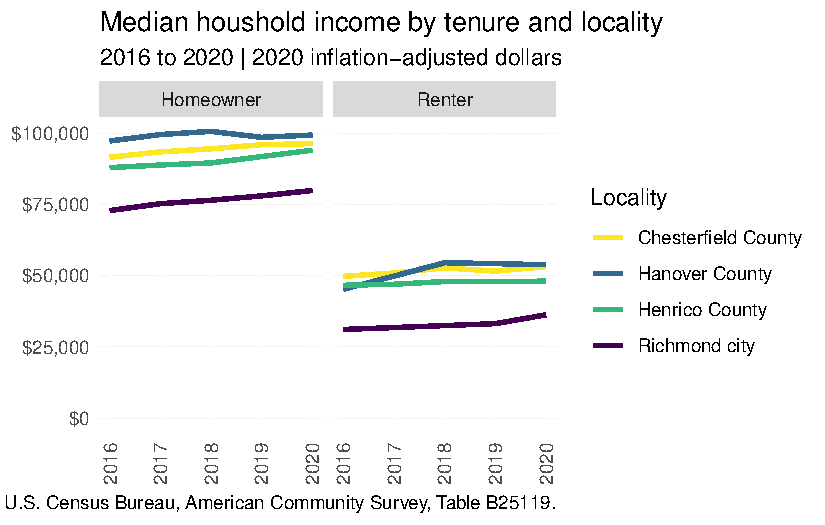
\includegraphics{./part-1-3_files/figure-pdf/fig-med-income-plot-1.pdf}

}

\caption{\label{fig-med-income-plot}Median houshold income by tenure and
locality}

\end{figure}

\begin{tcolorbox}[enhanced jigsaw, colframe=quarto-callout-important-color-frame, arc=.35mm, bottomrule=.15mm, colbacktitle=quarto-callout-important-color!10!white, opacityback=0, left=2mm, rightrule=.15mm, title=\textcolor{quarto-callout-important-color}{\faExclamation}\hspace{0.5em}{Adjusting for inflation}, colback=white, coltitle=black, toptitle=1mm, leftrule=.75mm, titlerule=0mm, breakable, opacitybacktitle=0.6, toprule=.15mm, bottomtitle=1mm]

When comparing dollar figures at different points in time, it is
important to account for the effects of
\href{https://www.investopedia.com/ask/answers/042415/what-impact-does-inflation-have-time-value-money.asp}{inflation}
on the dollar value. The value of a dollar in 2020 is not the same as in
2010 because inflation increases

To accurately compare data like median household incomes across time, we
must convert all dollar values to the same timeframe. The
\href{https://www.investopedia.com/terms/c/consumerpriceindex.asp}{Consumer
Price Index (CPI)} is used to adjust previous dollar figures to the most
recent data point.

\end{tcolorbox}

\hypertarget{incomes-by-race-and-ethnicity}{%
\subsection{Incomes by race and
ethnicity}\label{incomes-by-race-and-ethnicity}}

Typical incomes in the region remain unequal by race and ethnicity.
Households with the highest incomes include Asian and white,
non-Hispanic residents in the counties---earning well above \$75,000.
Black and Hispanic households consistently have the lowest median
incomes, along with multiracial households in Henrico and Richmond.

\begin{figure}

{\centering 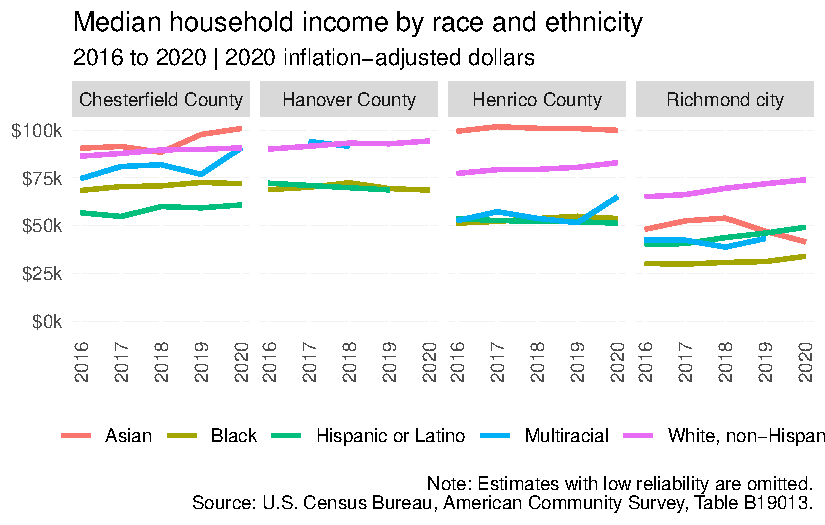
\includegraphics{./part-1-3_files/figure-pdf/fig-inc-race-plot-1.pdf}

}

\caption{\label{fig-inc-race-plot}Median household income by race and
ethnicity}

\end{figure}

\hypertarget{incomes-by-family-type}{%
\subsection{Incomes by family type}\label{incomes-by-family-type}}

Household incomes also vary by the presence of children or other related
individuals. Throughout the region, non-family households (i.e., persons
living alone or with unrelated persons) consistently have typical
incomes below \$50,000. In Henrico and Chesterfield counties, families
living with and without children under 18 have very similar income
levels. This trend is different in Hanover, where families with children
have much higher incomes, as well as Richmond, where they have much
lower incomes.

\begin{figure}

{\centering 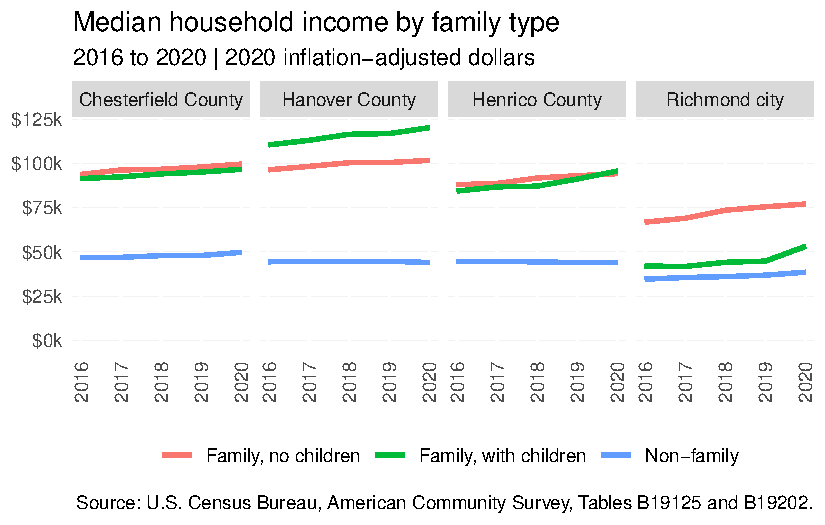
\includegraphics{./part-1-3_files/figure-pdf/fig-inc-child-plot-1.pdf}

}

\caption{\label{fig-inc-child-plot}Median household income by family
type}

\end{figure}

\hypertarget{wages}{%
\section{Wages}\label{wages}}

\begin{tcolorbox}[enhanced jigsaw, colframe=quarto-callout-note-color-frame, arc=.35mm, bottomrule=.15mm, colbacktitle=quarto-callout-note-color!10!white, opacityback=0, left=2mm, rightrule=.15mm, title=\textcolor{quarto-callout-note-color}{\faInfo}\hspace{0.5em}{Note}, colback=white, coltitle=black, toptitle=1mm, leftrule=.75mm, titlerule=0mm, breakable, opacitybacktitle=0.6, toprule=.15mm, bottomtitle=1mm]

Wage data in this section is sourced from the Occupational Employment
and Wage Statistics (OEWS) program of the Bureau of Labor Statistics.
OEWS is updated annually, most recently for 2021 data. This dataset
provides a rich look into wage distribution by industry and occupation.

However, OEWS is only available at the national, state, and metro
levels. Therefore, the data below covers the full Richmond, Virginia
Metropolitan Statistical Area (MSA) rather than the (smaller) PHA
region.

\end{tcolorbox}

\hypertarget{wage-change-by-percentile}{%
\subsection{Wage change by percentile}\label{wage-change-by-percentile}}

While regional wages increased across the board from May 2019 to May
2021, the largest percent increases in average wages were among jobs
that paid at and below the median wage. In fact, the largest growth
occurred in the lowest 10th percentile of wages, due in large part to
state lawmakers adopting incremental increases to Virginia's minimum
wage in 2020. The first increase from \$7.25 to \$9.50 per hour took
effect in 2021.

\begin{tcolorbox}[enhanced jigsaw, colframe=quarto-callout-note-color-frame, arc=.35mm, bottomrule=.15mm, colbacktitle=quarto-callout-note-color!10!white, opacityback=0, left=2mm, rightrule=.15mm, title=\textcolor{quarto-callout-note-color}{\faInfo}\hspace{0.5em}{Note}, colback=white, coltitle=black, toptitle=1mm, leftrule=.75mm, titlerule=0mm, breakable, opacitybacktitle=0.6, toprule=.15mm, bottomtitle=1mm]

Today, state minimum wage is \$11.00 per hour. Under
\href{https://lis.virginia.gov/cgi-bin/legp604.exe?201+sum+SB7}{current
law}, it will increase again to \$12.00 in 2023. Lawmakers must reenact
the measure by July 2024 to initiative further increases to \$15.00 per
hour by 2026.

\end{tcolorbox}

Another factor in this low-end wage growth is likely the
\href{https://www.bls.gov/opub/ted/2022/24-percent-of-establishments-increased-pay-or-paid-bonuses-because-of-covid-19-pandemic.htm}{increased
pay} offered by many businesses, especially in the food, retail, and
accommodation sectors, to encourage workers to return during the
COVID-19 recovery.

\begin{figure}

{\centering 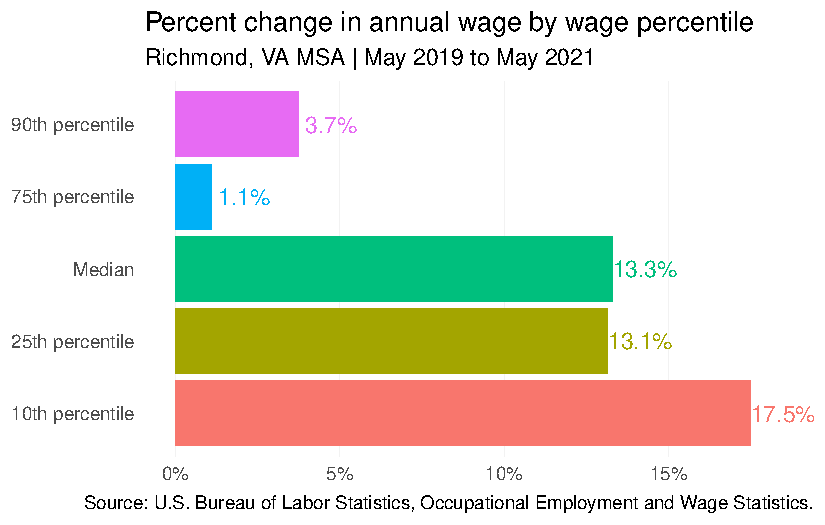
\includegraphics{./part-1-3_files/figure-pdf/fig-wage-pct-plot-1.pdf}

}

\caption{\label{fig-wage-pct-plot}Percent change in annual wage in
Richmond, VA MSA}

\end{figure}

\hypertarget{wage-change-by-occupation}{%
\subsection{Wage change by occupation}\label{wage-change-by-occupation}}

Over this same period, wages in the region grew for four of the five
most common occupation categories by total employment numbers. Workers
in the Transportation and Material Moving sector saw the largest
increases---from an average annual salary of \$30,250 to \$36,370 (over
20 percent).

Jobs in Food Preparation and Serving, Sales, and Business and Financial
Operations sectors---totaling more than 162,000 workers in the region as
of May 2021---also saw wage growth, but less than the 13.3 percent
average increase. Meanwhile, wages among Office and Administrative
Support positions remained nearly the same (-0.2 percent) from 2019 to
2021.

\begin{figure}

{\centering 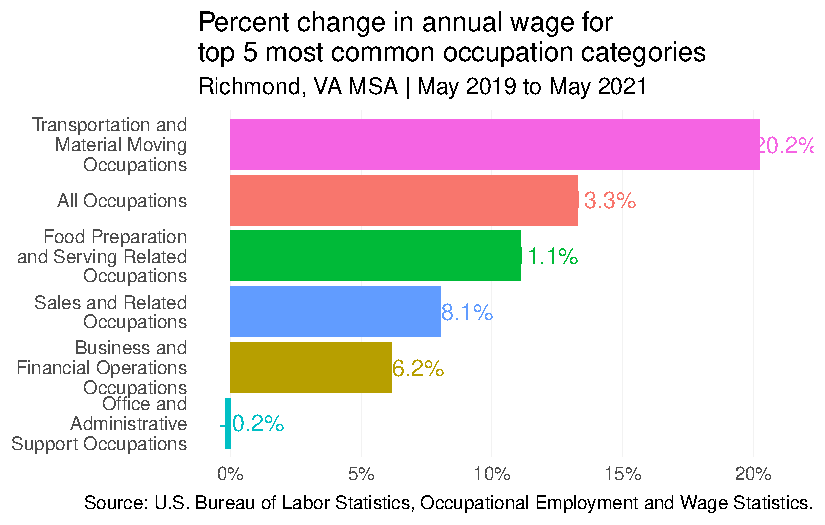
\includegraphics{./part-1-3_files/figure-pdf/fig-wage-occ-plot-1.pdf}

}

\caption{\label{fig-wage-occ-plot}Percent change in annual wage for top
5 most common occupation categories}

\end{figure}

\hypertarget{part-1-4}{%
\chapter{Special populations}\label{part-1-4}}

This chapter covers trends among populations that experience a
disability that may impact their ability to access and maintain housing.

\hypertarget{independent-living-difficulty}{%
\section{Independent living
difficulty}\label{independent-living-difficulty}}

In the American Community Survey (ACS), the Census Bureau collects a
range of characteristics to capture the range of different disability
types found in the population. One important disability type available
in ACS data is \emph{independent living difficulty}, which includes
persons who:

\begin{quote}
\emph{Because of a physical, mental, or emotional problem, {[}have{]}
difficulty doing errands alone such as visiting a doctor's office or
shopping.}
\end{quote}

As a result, persons with these difficulties often face significant
housing challenges as well.

\hypertarget{by-age}{%
\subsection{By age}\label{by-age}}

From 2016 to 2020, the region added almost 2,600 more persons with
independent living difficulties. The largest increases occurred among
young adults under 35, as well as ``young'' seniors between 65 and 74.
The latter group will see their needs increase acutely in the next
decade as they continue to age and potentially become more dependent on
others.

\begin{figure}

{\centering 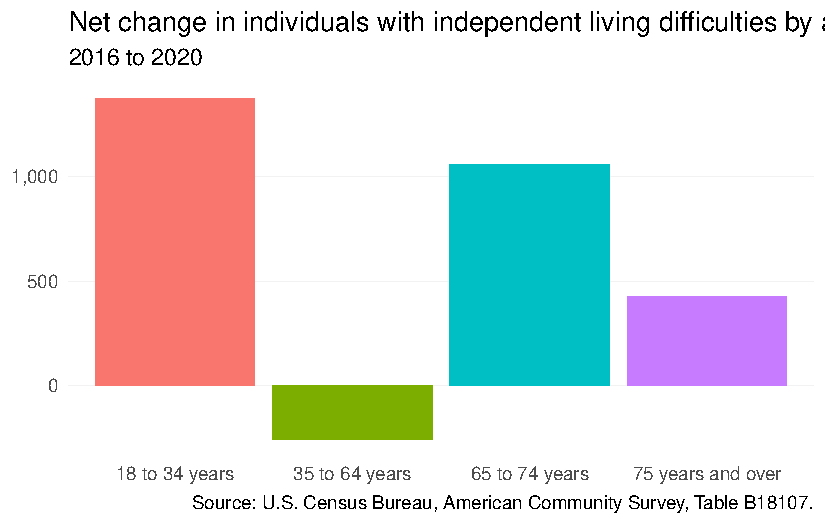
\includegraphics{./part-1-4_files/figure-pdf/fig-ind-liv-age-plot-1.pdf}

}

\caption{\label{fig-ind-liv-age-plot}Net change in individuals with
independent living difficulties by age}

\end{figure}

\hypertarget{by-tenure}{%
\subsection{By tenure}\label{by-tenure}}

\begin{tcolorbox}[enhanced jigsaw, colframe=quarto-callout-note-color-frame, arc=.35mm, bottomrule=.15mm, colbacktitle=quarto-callout-note-color!10!white, opacityback=0, left=2mm, rightrule=.15mm, title=\textcolor{quarto-callout-note-color}{\faInfo}\hspace{0.5em}{Note}, colback=white, coltitle=black, toptitle=1mm, leftrule=.75mm, titlerule=0mm, breakable, opacitybacktitle=0.6, toprule=.15mm, bottomtitle=1mm]

The detailed estimates for persons with independent living difficulties
in this and the next section are not available from the standard ACS
tables published by the Census Bureau. The data in these sections come
from the Public Use Microdata Sample (PUMS), which are available only by
special Public Use Microdata Areas (PUMAs) which contain at least
100,000 people.

While PUMA boundaries align with Chesterfield County, Henrico County,
and Richmond city, the PUMA containing Hanover County also includes
Powhatan, Goochland, New Kent, King William, Charles City counties.

\end{tcolorbox}

Nearly all persons with independent living difficulties throughout the
region live in regular homes, and not assisted living facilities or
other group quarters. Most are in homes that they own, or in homes owned
by another occupant, such as a spouse. This is not the case in Richmond,
however, where about half live in rented homes.

\begin{figure}

{\centering 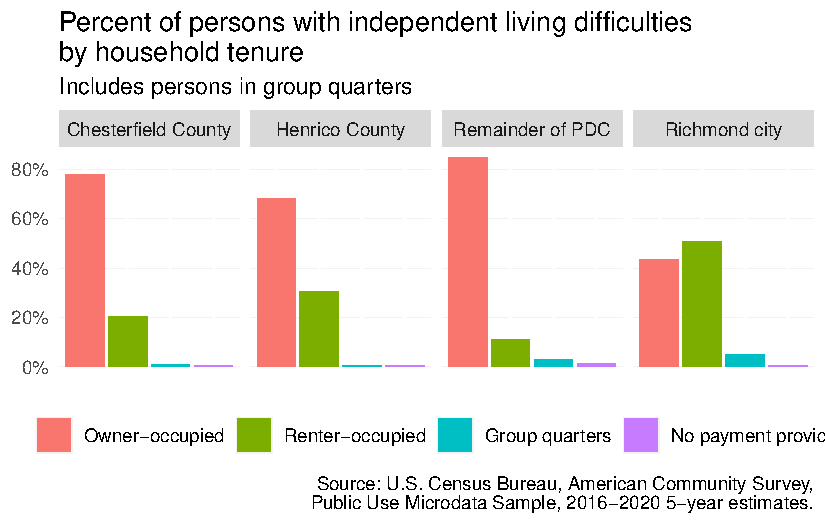
\includegraphics{./part-1-4_files/figure-pdf/fig-ind-liv-tenure-plot-1.pdf}

}

\caption{\label{fig-ind-liv-tenure-plot}Percent of persons with
independent living difficulties by household tenure}

\end{figure}

\hypertarget{by-household-size}{%
\subsection{By household size}\label{by-household-size}}

Persons with independent living difficulties are most likely to live
with one other person in their home. Slightly larger households (3 to 4
persons total) are also common. Still, more than 15 percent live
alone---including nearly one-in-four in Richmond. However, based on ACS
data collection methods, ``living alone'' also includes persons residing
in group quarters.

\begin{figure}

{\centering 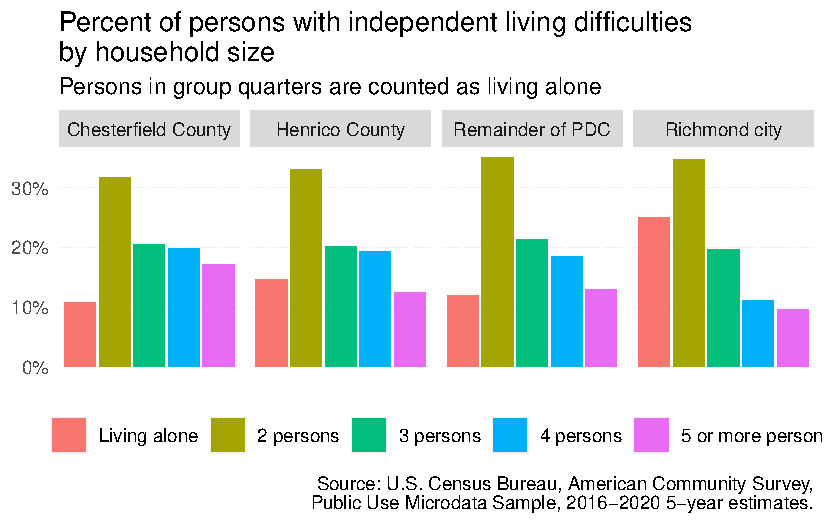
\includegraphics{./part-1-4_files/figure-pdf/fig-ind-liv-size-plot-1.pdf}

}

\caption{\label{fig-ind-liv-size-plot}Percent of persons with
independent living difficulties by household size}

\end{figure}

\hypertarget{veterans-with-disabilities}{%
\section{Veterans with disabilities}\label{veterans-with-disabilities}}

Veterans of military service have access to a range of Department of
Veterans Administration (VA) benefits, including VA home loans. These
benefits also include disability payments for veterans with
service-connected disabilities.

To award disability benefits, the VA assigns each disabled veteran a
\href{https://www.va.gov/disability/about-disability-ratings/}{rating}
from zero to 100 percent based on the severity of their disability or
disabilities. A higher rating reflects more significant impairments, and
accordingly, additional paid benefits to cover lost wages and extra
healthcare services.

From 2016 to 2020, the number of veterans in the region with a
service-connected disability increased by more than 2,800. A significant
majority of this growth occurred among veterans with disability rating
of 70 percent or higher, or those with the most severe physical and/or
mental health challenges.

Despite the increased benefits level associated with the higher rating,
these disabled veterans may be challenged to find accessible and
affordable housing options without additional support.

\begin{figure}

{\centering 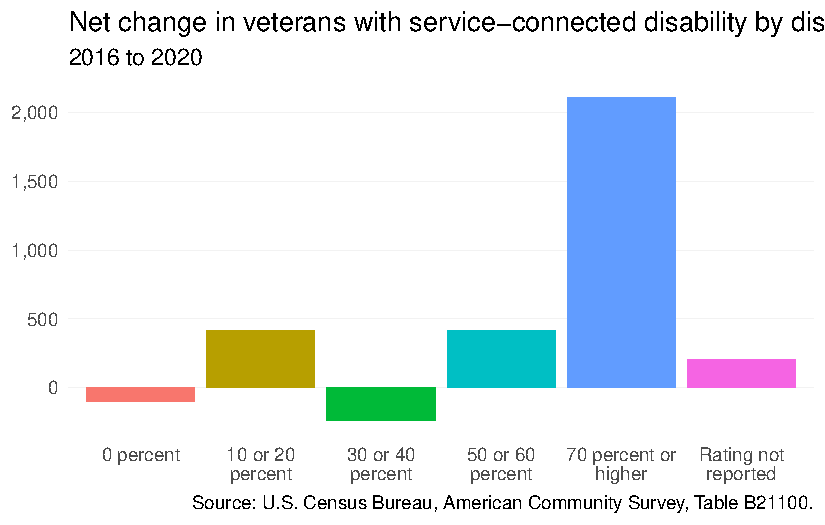
\includegraphics{./part-1-4_files/figure-pdf/fig-vets-plot-1.pdf}

}

\caption{\label{fig-vets-plot}Net change in veterans with
service-connected disability by disability rating}

\end{figure}

\part{PART 2: Housing supply and market changes}

\hypertarget{part-2-1}{%
\chapter{Homeownership}\label{part-2-1}}

This chapter covers the trends in the homeownership market across the
four main Partnership for Housing Affordability localities, including
the City of Richmond and counties of Chesterfield, Hanover, and Henrico.

\hypertarget{supply}{%
\section{Supply}\label{supply}}

\hypertarget{change-in-stock}{%
\subsection{Change in stock}\label{change-in-stock}}

The stock of homeowner housing has been growing across the region. From
2016 to 2020, owner-occupied housing has increased by 17,436---an
increase of seven percent. Unsurprisingly, much of that growth (93
percent) has occurred in the single-family home market, including
detached and attached homes. The largest share of that single-family
home growth has occurred in Chesterfield County, where there was a net
gain of 7,184 single-family owner-occupied homes.

\begin{figure}

{\centering \includegraphics{./part-2-1_files/figure-pdf/fig-oo-structure-plot-1.pdf}

}

\caption{\label{fig-oo-structure-plot}Change in owner-occupied housing
units by structure type}

\end{figure}

\hypertarget{age-of-stock}{%
\subsection{Age of stock}\label{age-of-stock}}

Between 2016 and 2020, almost all additions to the homeowner-occupied
housing stock in the region were, intuitively, homes built in the past
decade. However, there have also been thousands of net additions among
homes built before 1940 and between 1980 and 2009. These homes were most
likely previously occupied by renters and have now been reconverted into
homeownership opportunities.

\begin{figure}

{\centering \includegraphics{./part-2-1_files/figure-pdf/fig-oo-age-plot-1.pdf}

}

\caption{\label{fig-oo-age-plot}Change in owner-occupied housing units
by year built}

\end{figure}

\hypertarget{bedrooms}{%
\subsection{Bedrooms}\label{bedrooms}}

The majority of new owner-occupied homes in the region have three or
more bedrooms, continuing design and size trends prevalent since the mid
20th century. At the same time, homeowner households have become
smaller, which creates a surplus of largely unused bedrooms across the
market.

Smaller housing options exist largely in the City of Richmond or Henrico
County. While single-family homes---or condo units---with one- or two-
bedrooms are usually much more affordable, these housing options are
often in older, but highly desirable neighborhoods in the City of
Richmond (i.e., The Fan and Church Hill).

\begin{figure}

{\centering \includegraphics{./part-2-1_files/figure-pdf/fig-oo-beds-plot-1.pdf}

}

\caption{\label{fig-oo-beds-plot}Change in owner-occupied housing units
by number of bedrooms}

\end{figure}

\hypertarget{production}{%
\subsection{Production}\label{production}}

All localities in the region experienced single-family construction
declines as a result of the Great Recession from late 2007 to early 2012
--- especially Chesterfield and Henrico. Recovery has been unevenly
distributed, however.

From 2010 onward, every locality has seen increasing single-family home
construction, but the steepest increase has been in Chesterfield County.
From 2010 to 2020, single-family home construction has gone from 545
units to 2,202 per year in a decade --- a 300\% increase. Although
Chesterfield County was on its way to pre-Recession levels, all other
localities are seeing slow growth in the single-family home construction
space.

\begin{figure}

{\centering \includegraphics{./part-2-1_files/figure-pdf/fig-bps-plot-1.pdf}

}

\caption{\label{fig-bps-plot}Single-family building permits}

\end{figure}

\hypertarget{homeownership-rate}{%
\section{Homeownership rate}\label{homeownership-rate}}

\hypertarget{by-locality}{%
\subsection{By locality}\label{by-locality}}

Since 2016, overall homeownership rates for localities in the region
have increased slightly. This accounts for the net increase in
homeowners (over 15,000) and relatively steady number of renters over
this time period.

\begin{figure}

{\centering 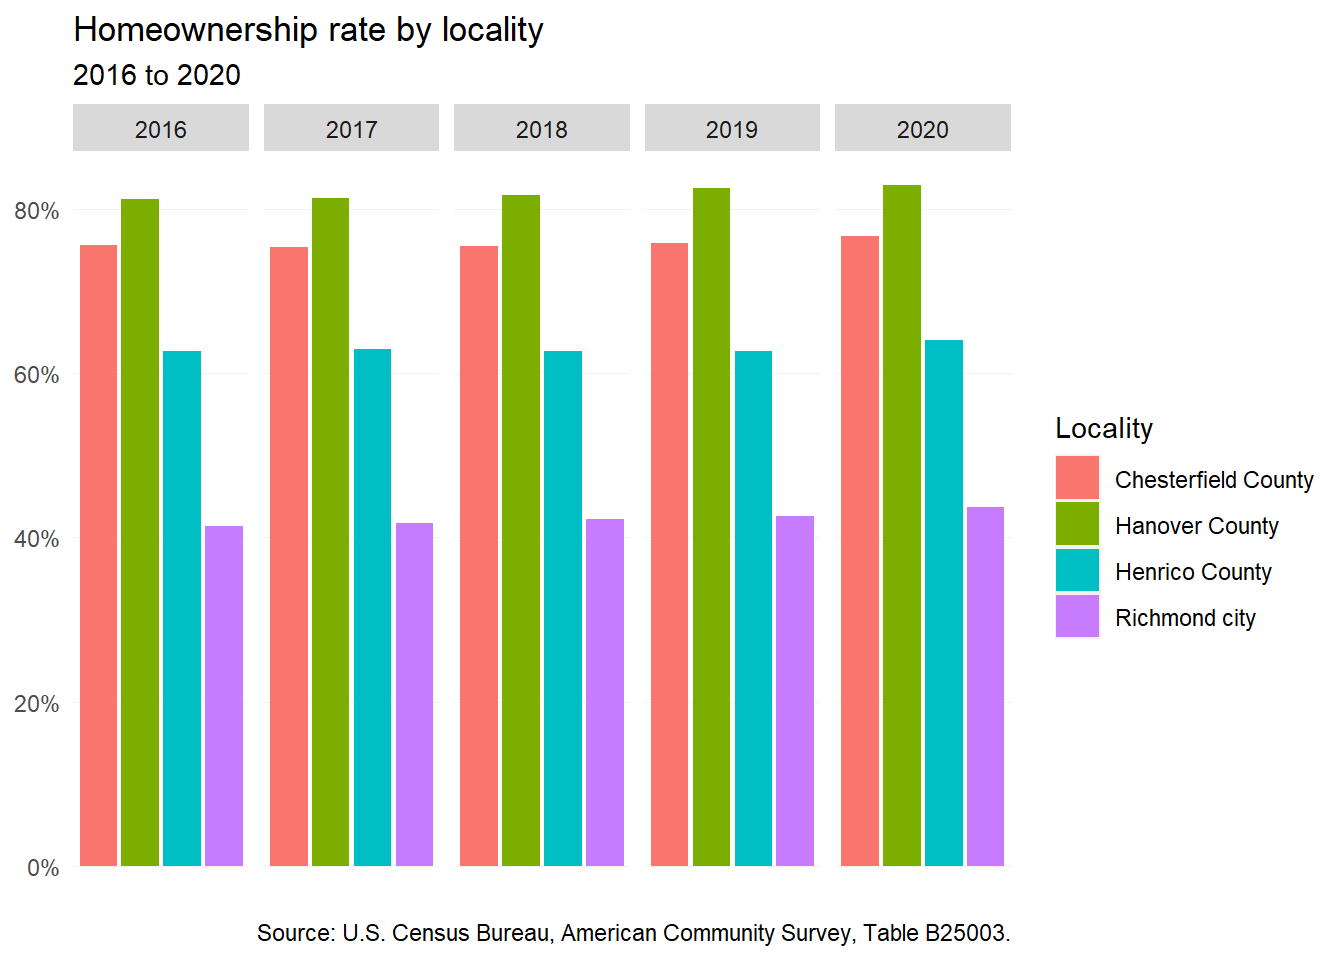
\includegraphics{./part-2-1_files/figure-pdf/fig-ho-rate-plot-1.pdf}

}

\caption{\label{fig-ho-rate-plot}Homeownership rate by locality}

\end{figure}

\hypertarget{by-age-1}{%
\subsection{By age}\label{by-age-1}}

Despite high rents, high debt, and low inventory, younger households
(under 35) have made some progress toward homeownership since 2016.
Their homeownership rate across the region increased from 30 to 35
percent. On the other hand, homeownership rates for middle-age and older
households remained about the same from 2016 to 2020.

\begin{figure}

{\centering \includegraphics{./part-2-1_files/figure-pdf/fig-ho-age-plot-1.pdf}

}

\caption{\label{fig-ho-age-plot}Homeownership rate by age group}

\end{figure}

\hypertarget{by-race-and-ethnicity}{%
\subsection{By race and ethnicity}\label{by-race-and-ethnicity}}

Across the region, the homeownership gap remains wide between white
households and households of color. White households in the Richmond
area are the only group with a homeownership rate above 70 percent.
However, several other groups---including Asian, multiracial, and Black
households---have seen slight increases in their homeownership rates
since 2016. At the same time, homeownership rates have fallen slightly
for Hispanic or Latino households and those of another race.

\begin{figure}

{\centering \includegraphics{./part-2-1_files/figure-pdf/fig-ho-race-plot-1.pdf}

}

\caption{\label{fig-ho-race-plot}Homeownership rate by race and
ethnicity}

\end{figure}

\hypertarget{for-sale-market}{%
\section{For-sale market}\label{for-sale-market}}

\hypertarget{closed-sales}{%
\subsection{Closed sales}\label{closed-sales}}

Home sales in the region continued to follow seasonal patterns during
the COVID-19 pandemic. All localities saw reductions in typical sales
volumes during early parts of the pandemic (spring to early summer
2020)---no doubt a result of stay-at-home orders. But by 2021, sales
volume began to climb back as
\href{https://www.marketwatch.com/story/mortgage-rates-drop-to-new-record-low-as-coronavirus-cases-climb-11605802099}{historically
low interest rates} incentivized home buying.

\begin{figure}

{\centering \includegraphics{./part-2-1_files/figure-pdf/fig-sales-plot-1.pdf}

}

\caption{\label{fig-sales-plot}Monthly home sales by locality}

\end{figure}

Chesterfield County continued to lead the region in home sales---hitting
a monthly peak in June 2021, with a total of 809 sales. In nearly all
localities except for Chesterfield County, the average monthly home
sales has largely remained the same. Only in Chesterfield County was
there a more than 10 percent increase in average monthly home sales
between 2019 and 2021.

\begin{figure}

{\centering \includegraphics{./part-2-1_files/figure-pdf/fig-sales-avg-plot-1.pdf}

}

\caption{\label{fig-sales-avg-plot}Average monthly home sales by
locality}

\end{figure}

\hypertarget{sales-price}{%
\subsection{Sales price}\label{sales-price}}

Median home prices have continued to climb in the Richmond
Region---reaching over \$300,000 in all four major localities. The
greatest price increases have occurred in the City of Richmond during
2022, where the median home price went from \$303,941 in February to
\$389,950 in June, a 28 percent increase. Home prices continue to remain
high in spite of
\href{https://www.nar.realtor/magazine/real-estate-news/economy/mortgage-rates-october-20-2022}{rising
mortgage interest rates}.

Hanover County remains the most expensive locality in the region with a
median home price of \$423,250 as of September 2022, followed by the
Chesterfield County (\$371,273), Henrico County (\$349,950), and the
City of Richmond (\$325,500).

\begin{figure}

{\centering \includegraphics{./part-2-1_files/figure-pdf/fig-sales-price-plot-1.pdf}

}

\caption{\label{fig-sales-price-plot}Monthly median sales price by
locality}

\end{figure}

\hypertarget{supply-1}{%
\subsection{Supply}\label{supply-1}}

The inventory of for-sale housing before the pandemic typically sat at
two months or more---meaning that it would take two or more months to
sell at current prices. A healthy level of supply has said to be five or
six months worth, but in recent years the region has been below that,
which indicates a strong seller's market.

When pandemic began in March 2020, months supply dropped to two months
and then by June 2020 hit a low of one month and has sat squarely there
ever since. Even amid rising interest rates in 2022 and talks of a
housing slump, months supply continues to remain low.

\begin{figure}

{\centering \includegraphics{./part-2-1_files/figure-pdf/fig-supply-plot-1.pdf}

}

\caption{\label{fig-supply-plot}Months of supply}

\end{figure}

\hypertarget{starter-homes}{%
\subsection{Starter homes}\label{starter-homes}}

Starter homes provide young adults the ability to get on the first rung
of the homeownership ladder. This allows many young adults the ability
to build equity before their household grows (i.e.~marriage and
children). But starter homes are becoming more and more scarce. This has
largely been the result of starter home opportunities not coming to
market. In some cases, older homes occupied by seniors are not hitting
the market because senior desire to age-in-place remains high or seniors
simply cannot find other affordable options themselves. Starter homes
are also ripe for investor flipping, which leaves first-time homebuyers
competing with all cash offers.

In addition, smaller homes do not make up a significant share of new
construction stock. Smaller homes (two-bedroom or less) are often more
desirable among seniors and young adults without children. The lack of
this stock prevents the movement of households from different rungs
along the homeownership ladder --- locking homeowners into homes that
often no longer work for them.

In 2021, the Virginia REALTORS® (VAR) conducted an analysis of the
number and share of starter homes sold in Virginia from 2013 to
mid-2021. This analysis was included in the statewide housing study
conducted by HousingForward Virginia as part of
\href{https://dmz1.dhcd.virginia.gov/HB854/part-3-homeownership.html\#finding-2-starter-home-inventory-is-decreasing.}{HB
854}. To calculate the number and share of starter homes sold, VAR
calculated the number of homes sold that would be affordable to a
household making 80 percent of AMI.

For the region, the share of starter homes sold has been in a steady
decline. The greatest decrease has occurred in Chesterfield County,
where the share of starter homes sold has gone from 63 percent to 46
percent. The smallest decrease occurred in Henrico County, a decrease of
only 8 percentage points.

\begin{figure}

{\centering \includegraphics{./part-2-1_files/figure-pdf/fig-starter-plot-1.pdf}

}

\caption{\label{fig-starter-plot}Share of sold homes affordable to 80\%
AMI}

\end{figure}

\hypertarget{new-construction-versus-resale}{%
\section{New construction versus
resale}\label{new-construction-versus-resale}}

\hypertarget{sales-price-1}{%
\subsection{Sales price}\label{sales-price-1}}

The affordability of resale homes compared to new construction has often
made them the first rung on the homeownership ladder. But since the
start of the pandemic, the median resale home price has risen above the
\$300,000 mark and in June 2022 reached a high of \$371,250.

During this timeframe, new construction median home prices have remained
above \$350,000 and throughout 2022 so far have stayed above \$400,000.
On average, there is a \$89,127 difference between new construction and
resale sales price---leaving new construction significantly out of reach
for lower income households.

\begin{figure}

{\centering \includegraphics{./part-2-1_files/figure-pdf/fig-comp-price-plot-1.pdf}

}

\caption{\label{fig-comp-price-plot}Median price of new construction and
resale}

\end{figure}

\hypertarget{bedrooms-1}{%
\subsection{Bedrooms}\label{bedrooms-1}}

The majority of home sales in the region have been for three- and
four-bedroom homes --- roughly three in four homes sold in the past five
years. Nuances exist at either end of the bedroom spectrum.

New construction with one- to two-bedrooms has been increasing --- going
from six percent of sales in 2017 to nine percent in 2022 YTD. At the
other end, new construction of five or more bedroom homes has increased
as well with an increase of three percent (15 percent of sales in 2017
to 18 percent in 2022 YTD). For resale homes, the share of homes by
bedroom has remained largely unchanged each year.

\begin{figure}

{\centering \includegraphics{./part-2-1_files/figure-pdf/fig-comp-br-plot-1.pdf}

}

\caption{\label{fig-comp-br-plot}Share of bedrooms by new construction
and resales}

\end{figure}

\hypertarget{size}{%
\subsection{Size}\label{size}}

In the past five years, there have been clear differences in new
construction and resale sales by square footage. The majority of resale
homes have been under 2,000 square feet, while new construction is
overwhelmingly over 2,000 square feet. These differences have clear
implications on home prices (i.e.~more square footage means higher
prices). But across the region, minimum requirements set out by
localities in zoning ordinances impact these builder decisions.

\href{https://archive.curbed.com/2020/3/10/21168519/homes-for-sale-american-home-suburbs}{Building
smaller homes} is less profitable given the rising cost to develop a
single detached home (e.g.~rising land, infrastructure, and regulatory
costs). In order to maximize profit, home builders need to increase
square footage to recoup costs and meet development requirements.

\begin{figure}

{\centering \includegraphics{./part-2-1_files/figure-pdf/fig-comp-sf-plot-1.pdf}

}

\caption{\label{fig-comp-sf-plot}Home size by new construction and
resales}

\end{figure}

\hypertarget{part-2-2}{%
\chapter{Rental homes}\label{part-2-2}}

This chapter covers trends in the rental housing market across the four
main Partnership for Housing Affordability localities, including the
City of Richmond and counties of Chesterfield, Hanover, and Henrico.

\hypertarget{supply-2}{%
\section{Supply}\label{supply-2}}

\hypertarget{change-in-stock-1}{%
\subsection{Change in stock}\label{change-in-stock-1}}

While many renters across the region do live in multifamily buildings
(with 5 or more units), the second largest share of rental housing is
single-family housing (either attached or detached). In 2020, over a
third (37 percent) of rental housing in the region consisted of
single-family housing, while 49 percent was located in buildings with 5
or more units. There has been little change in these percentages since
2016.

Changes in the shares of rental housing have been small --- but those
changes have been among rental housing with 20 or more units (17 percent
in 2016 to 19 percent in 2020) and 2 to 4 unit buildings (14 percent in
2016 down to 13 percent in 2020).

\begin{figure}

{\centering 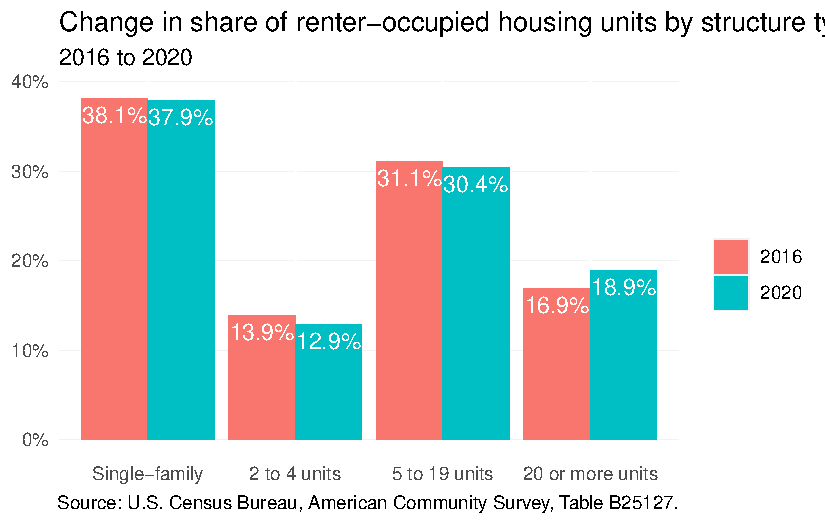
\includegraphics{./part-2-2_files/figure-pdf/fig-ro-structure-percent-1.pdf}

}

\caption{\label{fig-ro-structure-percent}Change in share of
renter-occupied housing units by structure type}

\end{figure}

The raw changes in rental housing were most felt in Henrico County and
the City of Richmond. In Henrico, there was a 1,930 increase in
single-family rental housing and a 1,357 decrease in 2 to 4 unit rental
housing (i.e.~duplexes, triplexes, and quads).

The City of Richmond saw a contrasting decrease in single-family rentals
(-1,921), while also experiencing a 2,134 increase in rental housing
located in buildings with 20 or more units. Chesterfield County has seen
slight increases in multifamily housing of all types, while Hanover
County has not seen much change at all.

\begin{figure}

{\centering 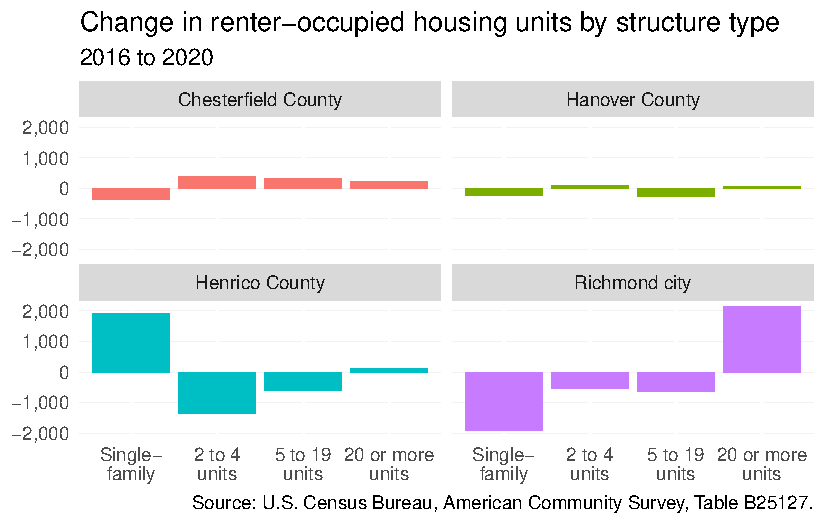
\includegraphics{./part-2-2_files/figure-pdf/fig-ro-structure-1.pdf}

}

\caption{\label{fig-ro-structure}Change in renter-occupied housing units
by structure type}

\end{figure}

\hypertarget{age-of-stock-1}{%
\subsection{Age of stock}\label{age-of-stock-1}}

Since 2016, the region has seen major changes in the age of its rental
stock as existing homes transition from being owned to leased out, or
vice-versa. Of note, every locality except for Hanover saw significant
increases in the number of renter-occupied homes built between 1980 and
1999.

These homes---now over 20 years old---are likely becoming the target of
investors purchasing from homeowners, making certain improvements, and
renting them out. In Henrico County, this trend was even more prevalent
among homes built between 1960 and 1979.

\begin{tcolorbox}[enhanced jigsaw, colframe=quarto-callout-note-color-frame, arc=.35mm, bottomrule=.15mm, colbacktitle=quarto-callout-note-color!10!white, opacityback=0, left=2mm, rightrule=.15mm, title=\textcolor{quarto-callout-note-color}{\faInfo}\hspace{0.5em}{Market Value Analysis (MVA)}, colback=white, coltitle=black, toptitle=1mm, leftrule=.75mm, titlerule=0mm, breakable, opacitybacktitle=0.6, toprule=.15mm, bottomtitle=1mm]

In 2021, Richmond Memorial Health Foundation (RMHF) and PlanRVA
commissioned a second Market Value Analysis (MVA) of the Richmond
region. The MVA is a ``is a data-based, field-validated analysis and
mapping of a community's housing market.'' Richmond's MVA provides
fine-grained data analysis of neighborhood changes and trends, including
residential vacancy and investor sales.

Learn more about the MVA
\href{https://rmhfoundation.org/resource/richmond-memorial-health-foundation-co-sponsored-analysis-of-the-richmond-areas-housing-market-reveals-important-trends-for-residents-policymakers-and-investors/}{here}.

\end{tcolorbox}

Conversely, Chesterfield and Henrico each had over 1,000 homes built
between 2000 and 2009 change from renter- to owner-occupied. The largest
losses in rental stock, however, occurred in Richmond among homes built
prior to 1980. Several factors could explain this decline:

\begin{itemize}
\tightlist
\item
  Actual demolition of very old, low-quality homes,
\item
  Duplexes and triplexes converted into single-family homes, and
\item
  Single-family rentals purchased by buyers who now live in the home.
\end{itemize}

\begin{figure}

{\centering 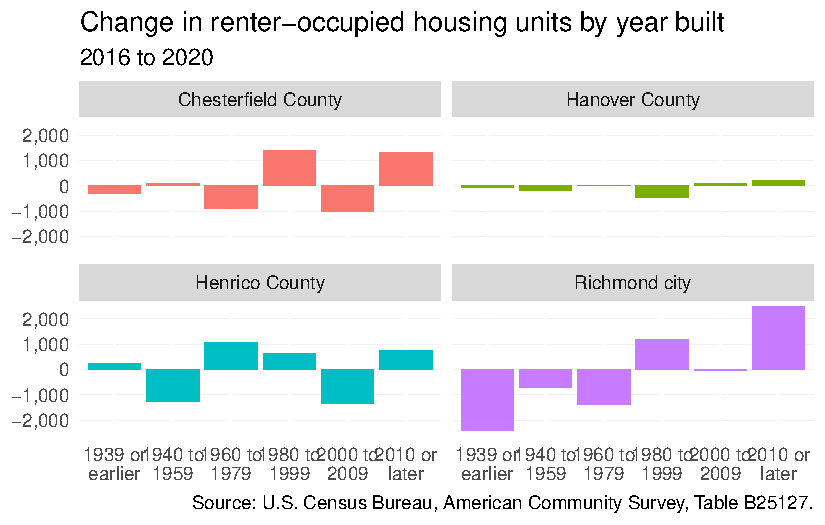
\includegraphics{./part-2-2_files/figure-pdf/fig-ro-year-built-1.pdf}

}

\caption{\label{fig-ro-year-built}Change in renter-occupied housing
units by year built}

\end{figure}

\hypertarget{bedrooms-2}{%
\subsection{Bedrooms}\label{bedrooms-2}}

Rental homes in the Richmond region are most likely to have one or two
bedrooms. While the number of one-bedroom apartments has continued to
increase (+1,617) from 2016, the number of two-bedroom units has
decreased by 2,500.

The increasing supply of one-bedroom apartments coincides with a similar
increase in studio apartments---these unit sizes reflect new apartments,
largely in Richmond, marketed for college students and other young
adults.

The dwindling number of two-bedroom rental homes may reflect small
single-family rentals in older neighborhoods transitioning to
owner-occupancy, as there is a similar (but much less significant)
decline in three-bedroom units.

\begin{figure}

{\centering 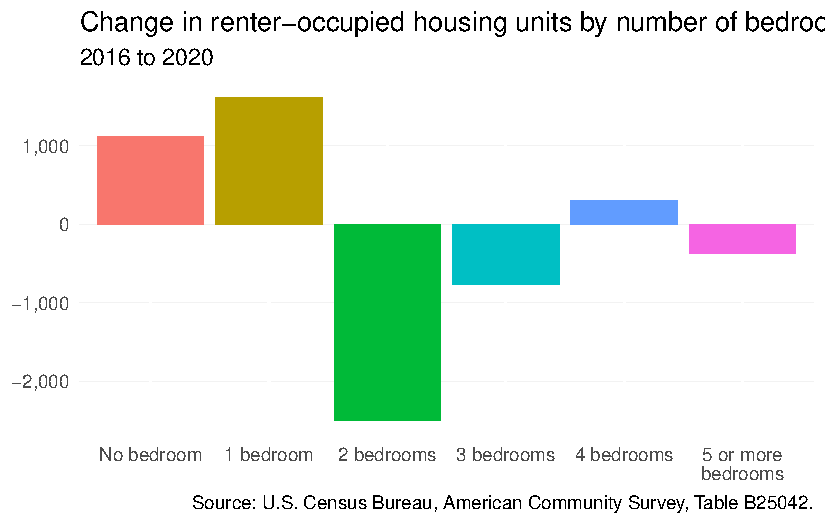
\includegraphics{./part-2-2_files/figure-pdf/fig-ro-bedrooms-1.pdf}

}

\caption{\label{fig-ro-bedrooms}Change in renter-occupied housing units
by number of bedrooms}

\end{figure}

\hypertarget{production-1}{%
\subsection{Production}\label{production-1}}

Construction of multifamily properties (with 5 units or more) has been
sporadic since the end of the Great Recession. In all localities aside
from Hanover County, there have been waves and dips in the multifamily
building construction. Hanover has seen little to no activity throughout
the last two decades, while Chesterfield County and Richmond have seen
the bulk of activity.

During the latter half of the last decade, Chesterfield County had a
boom in multifamily construction --- nearing 1,500 units in 2019.
Meanwhile, Richmond's multifamily construction saw dips following the
Great Recession and again in 2018, but has largely been up in the last
couple years of the 2010s. Although Henrico County had dips in 2016 and
2018, multifamily construction has more often than not been above the
700 unit mark.

\hypertarget{rental-market}{%
\section{Rental market}\label{rental-market}}

\hypertarget{average-market-asking-rent}{%
\subsection{Average market asking
rent}\label{average-market-asking-rent}}

Rental demand reached
\href{https://richmond.com/news/local/rent-in-richmond-region-surged-during-the-pandemic-two-bedroom-apartments-average-1-340-a/article_751d018b-b5b4-5592-9582-9e825bda674b.html}{a
fever pitch amid the ongoing COVID-19 pandemic}. With eviction
moratoriums and a flow of rental assistance, low supply gave way to
historic rent increases. The average market asking rent in the region
reached a two-decade high of \$1,395 in the first quarter of 2022.

\begin{figure}

{\centering 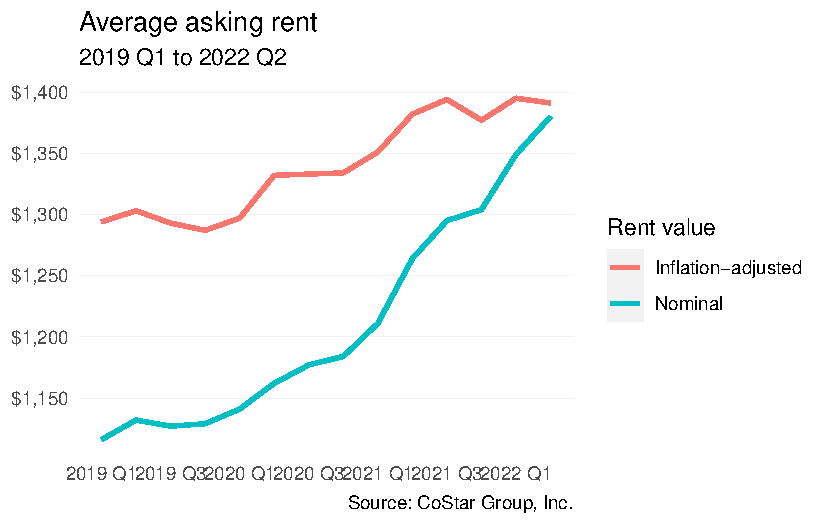
\includegraphics{./part-2-2_files/figure-pdf/fig-avg-rent-1.pdf}

}

\caption{\label{fig-avg-rent}Average asking rent}

\end{figure}

Large quarterly increases in average rents began in early 2021 and have
continued to the present. From the first to second quarters of this
year, rents increased by \$31. However, this relative growth was very
near the change in inflation over that same period.

\begin{figure}

{\centering 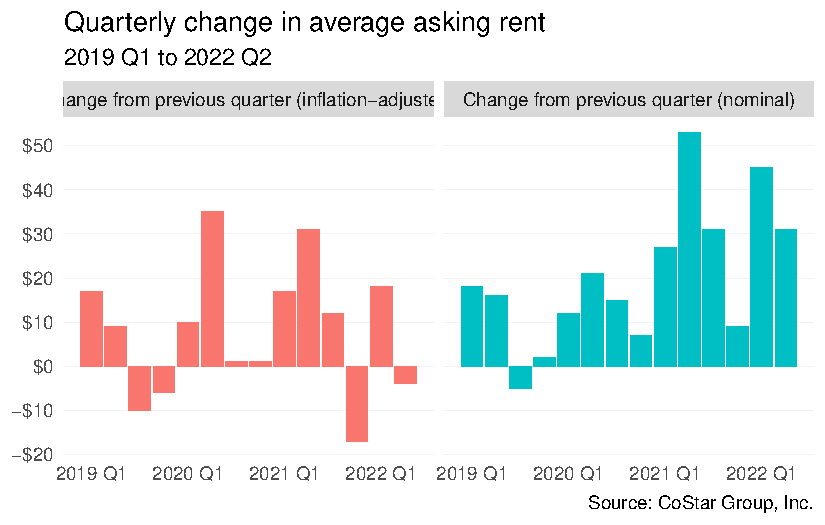
\includegraphics{./part-2-2_files/figure-pdf/fig-avg-rent-change-1.pdf}

}

\caption{\label{fig-avg-rent-change}Quarterly change in average asking
rent}

\end{figure}

\hypertarget{rents-by-submarket}{%
\subsection{Rents by submarket}\label{rents-by-submarket}}

Although not adjusted for inflation, rents by submarket show that there
are distinct average rents across the region. Since 2010, the steepest
increases have occurred in the counties. Northside Richmond remains the
least expensive submarket with an average rent of \$1,037 in the second
quarter of this year, while Midlothian is the most expensive at \$1,655.

\begin{figure}

{\centering 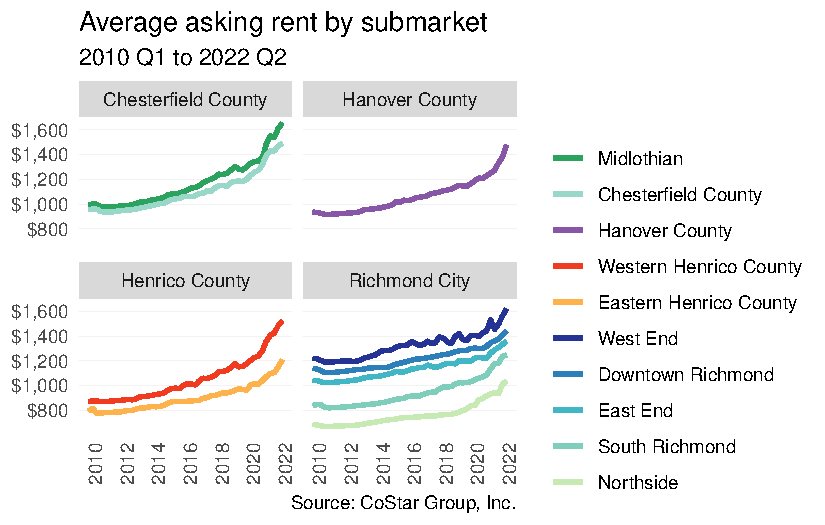
\includegraphics{./part-2-2_files/figure-pdf/fig-avg-rent-submarket-1.pdf}

}

\caption{\label{fig-avg-rent-submarket}Average asking rent by submarket}

\end{figure}

\hypertarget{rents-by-bedrooms}{%
\subsection{Rents by bedrooms}\label{rents-by-bedrooms}}

Rents in the region have risen the most among three-bedroom and
two-bedroom apartments, reflecting continued demand for units that have
actually \emph{declined} in supply since 2016. In contrast, average
rents for studio and one-bedroom apartments---which grew by more than
2,700 units since 2016---have increased less than \$100 over the last
decade when adjusted for inflation.

\begin{figure}

{\centering 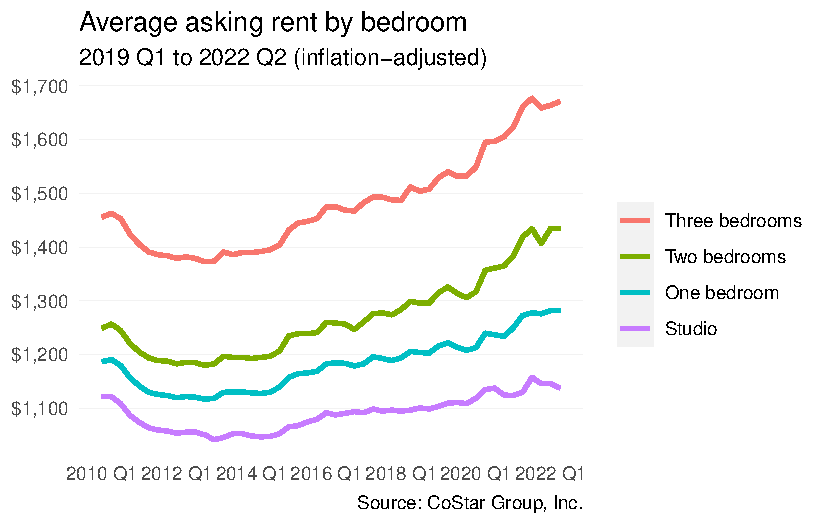
\includegraphics{./part-2-2_files/figure-pdf/fig-avg-rent-br-1.pdf}

}

\caption{\label{fig-avg-rent-br}Average asking rent by bedroom}

\end{figure}

\hypertarget{rents-by-age-of-units}{%
\subsection{Rents by age of units}\label{rents-by-age-of-units}}

Recently constructed rental housing (built in 2010 and after) leads
average asking rents at \$1,614. As expected, rental costs correlate to
the period in which they were built --- with older rental housing being
less expensive. Pre-1980 rental housing is roughly \$400 cheaper than
more recent rental housing.

In the last decade, more recent rental housing had steady and modest
increases; only increasing \$80 from Q1 2012 to Q2 2022. But older
rental housing had much more dramatic increases; increasing an average
of \$257 in that same time period.

Rental housing built between 1980 and 2009 had especially steep
increases during the height of the pandemic (Q1 2020 to Q3 2021). In
this time, the average asking rent increased by over \$130, while rent
increases for newer rental housing and pre-1980 housing increased by
less than \$100.

\begin{figure}

{\centering 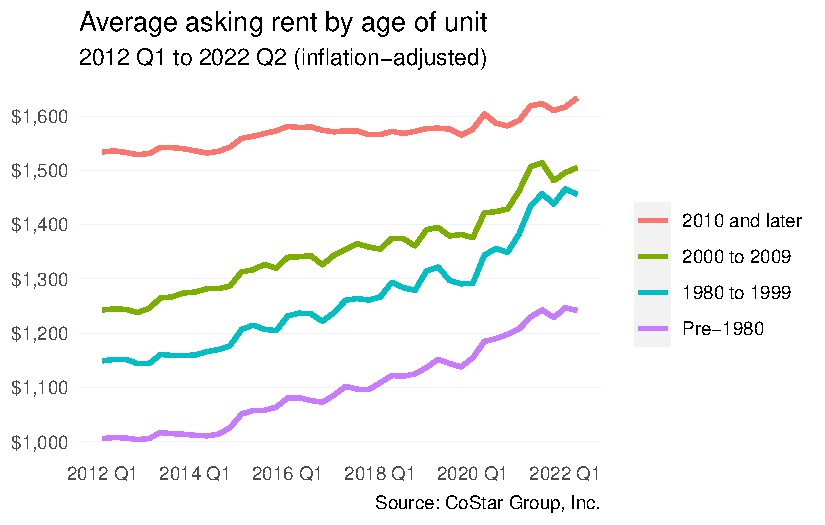
\includegraphics{./part-2-2_files/figure-pdf/fig-rents-built-1.pdf}

}

\caption{\label{fig-rents-built}Average asking rent by age of unit}

\end{figure}

\hypertarget{rental-vacancy}{%
\section{Rental vacancy}\label{rental-vacancy}}

For much of the past two decades, vacancy rates have fluctuated
seasonally as new people enter and leave the rental housing market.
Across the region, submarkets have largely had vacancy rates below ten
percent. In 2022, the regional average vacancy rate to-date was five
percent.

However, some submarkets in the region have lower than average vacancy
rates; Hanover County (1 percent), Eastern Henrico (3 percent),
Northside (3 percent), and East End (4 percent) have significantly lower
vacancy rates.

\begin{figure}

{\centering 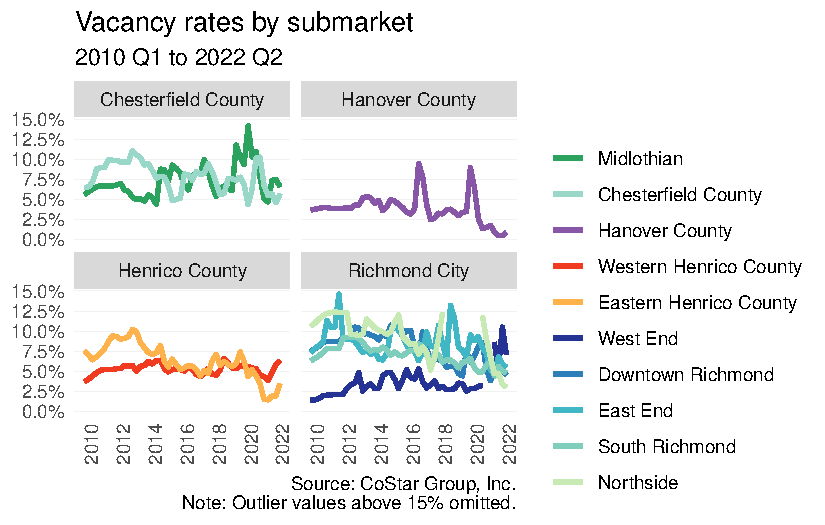
\includegraphics{./part-2-2_files/figure-pdf/fig-vacancy-1.pdf}

}

\caption{\label{fig-vacancy}Vacancy rates by submarket}

\end{figure}

\hypertarget{part-2-3}{%
\chapter{Housing assistance}\label{part-2-3}}

This chapter covers the range of housing assistance in the region
supported by federal, state, and local programs.

\hypertarget{affordable-rental-housing}{%
\section{Affordable rental housing}\label{affordable-rental-housing}}

An array of federal housing assistance programs help low-income
residents across the region with rental housing opportunities. Today,
there are approximately 25,969 dedicated affordable rental homes found
across 240 properties in the Richmond area. These include units both
currently occupied and in development.

\begin{tcolorbox}[enhanced jigsaw, colframe=quarto-callout-tip-color-frame, arc=.35mm, bottomrule=.15mm, colbacktitle=quarto-callout-tip-color!10!white, opacityback=0, left=2mm, rightrule=.15mm, title=\textcolor{quarto-callout-tip-color}{\faLightbulb}\hspace{0.5em}{Funding sources}, colback=white, coltitle=black, toptitle=1mm, leftrule=.75mm, titlerule=0mm, breakable, opacitybacktitle=0.6, toprule=.15mm, bottomtitle=1mm]

In the Richmond region, many affordable rental properties also receive
assistance from the Virginia Housing Trust Fund, as well as local
sources such as CDBG and HOME grants. The City of Richmond also awards
funding to affordable rental projects with its own trust fund. These
awards often fill a financing ``gap'' and do not provide a majority of
the total assistance for a development; as a result, they are not
specifically reflected in the data.

\end{tcolorbox}

\hypertarget{subsidy-types}{%
\subsection{Subsidy types}\label{subsidy-types}}

Over half (51 percent) of all affordable rental homes in the region rely
\emph{solely} on the LIHTC program. Another 31 percent have layered
multiple subsidies together, reflecting the capital and funding
requirements needed to develop new affordable housing.

The other significant source of dedicated affordable housing continues
to be more than 3,600 Public Housing units managed by Richmond
Redevelopment and Housing Authority.

\begin{tcolorbox}[enhanced jigsaw, colframe=quarto-callout-note-color-frame, arc=.35mm, bottomrule=.15mm, colbacktitle=quarto-callout-note-color!10!white, opacityback=0, left=2mm, rightrule=.15mm, title=\textcolor{quarto-callout-note-color}{\faInfo}\hspace{0.5em}{Note}, colback=white, coltitle=black, toptitle=1mm, leftrule=.75mm, titlerule=0mm, breakable, opacitybacktitle=0.6, toprule=.15mm, bottomtitle=1mm]

Descriptions of each rental assistance program are available on the
\href{https://preservationdatabase.org/documentation/program-descriptions/}{NHPD
website}.

\end{tcolorbox}

\begin{tcolorbox}[enhanced jigsaw, colframe=quarto-callout-important-color-frame, arc=.35mm, bottomrule=.15mm, colbacktitle=quarto-callout-important-color!10!white, opacityback=0, left=2mm, rightrule=.15mm, title=\textcolor{quarto-callout-important-color}{\faExclamation}\hspace{0.5em}{Important}, colback=white, coltitle=black, toptitle=1mm, leftrule=.75mm, titlerule=0mm, breakable, opacitybacktitle=0.6, toprule=.15mm, bottomtitle=1mm]

It is important to note that Section 8 described in this section is not
the same as Section 8 Housing Choice Vouchers. Section 8 subsidies
described in this section refer to HUD project-based rental assistance
--- meaning that they are rental assistance that is tied to a specific
development, whereas Section 8 Housing Choice Vouchers are tenant-based
subsidies that a recipient can take wherever they can find housing.

\end{tcolorbox}

\begin{figure}

{\centering 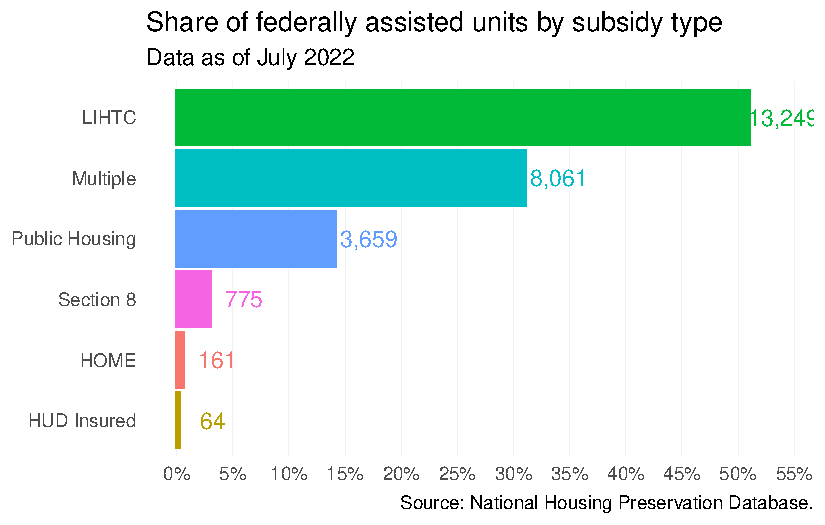
\includegraphics{./part-2-3_files/figure-pdf/fig-subsidy-overall-1.pdf}

}

\caption{\label{fig-subsidy-overall}Share of federally assisted units by
subsidy}

\end{figure}

\hypertarget{layered-subsidies}{%
\subsection{Layered subsidies}\label{layered-subsidies}}

In an effort to maximize assistance, rental subsidy programs are often
layered together into single projects. Among the 8,061 units with
multiple subsidies, over half have either a 4\% or 9\% LIHTC tax
credit---or both ``twinned'' together. Section 8 Housing Finance and
Development Agency (HFDA) New Construction and Loan Management Set-Aside
(LMSA) programs are also common types.

``Other'' subsidies generally include HUD insurance programs and other,
less common, Section 8 programs. Still, these minor assistance packages
nevertheless provide helping subsidy to almost three-in-four units with
multiple affordability contracts.

\hypertarget{tbl-multiple}{}
\begin{table}
\caption{\label{tbl-multiple}Active subsidies in units with mutiple subsidies }\tabularnewline

\centering
\begin{tabular}{l|r|r}
\hline
Detailed subsidy type & Units with subsidy & Percent of total\\
\hline
LIHTC 4\% Tax Credit & 4,747 & 58.9\%\\
\hline
LIHTC 9\% Tax Credit & 4,371 & 54.2\%\\
\hline
Section 8 HFDA/8 NC & 1,584 & 19.7\%\\
\hline
Section 8 LMSA & 1,173 & 14.6\%\\
\hline
Other & 5,880 & 72.9\%\\
\hline
\multicolumn{3}{l}{\rule{0pt}{1em}Sources: National Housing Preservation Database and Virginia Housing.}\\
\end{tabular}
\end{table}

\begin{tcolorbox}[enhanced jigsaw, colframe=quarto-callout-note-color-frame, arc=.35mm, bottomrule=.15mm, colbacktitle=quarto-callout-note-color!10!white, opacityback=0, left=2mm, rightrule=.15mm, title=\textcolor{quarto-callout-note-color}{\faInfo}\hspace{0.5em}{Note}, colback=white, coltitle=black, toptitle=1mm, leftrule=.75mm, titlerule=0mm, breakable, opacitybacktitle=0.6, toprule=.15mm, bottomtitle=1mm]

Table totals do not add to 100 percent because units are percent of all
8,061 \emph{units} with multiple subsidies, not the total of all
subsidies.

\end{tcolorbox}

\hypertarget{locations}{%
\subsection{Locations}\label{locations}}

The map below shows the locations of affordable rental properties in the
Richmond region. Each color corresponds to the property's subsidy as
recorded in the National Housing Preservation Database, or if multiple
subsidies are currently active.

\begin{figure}

{\centering 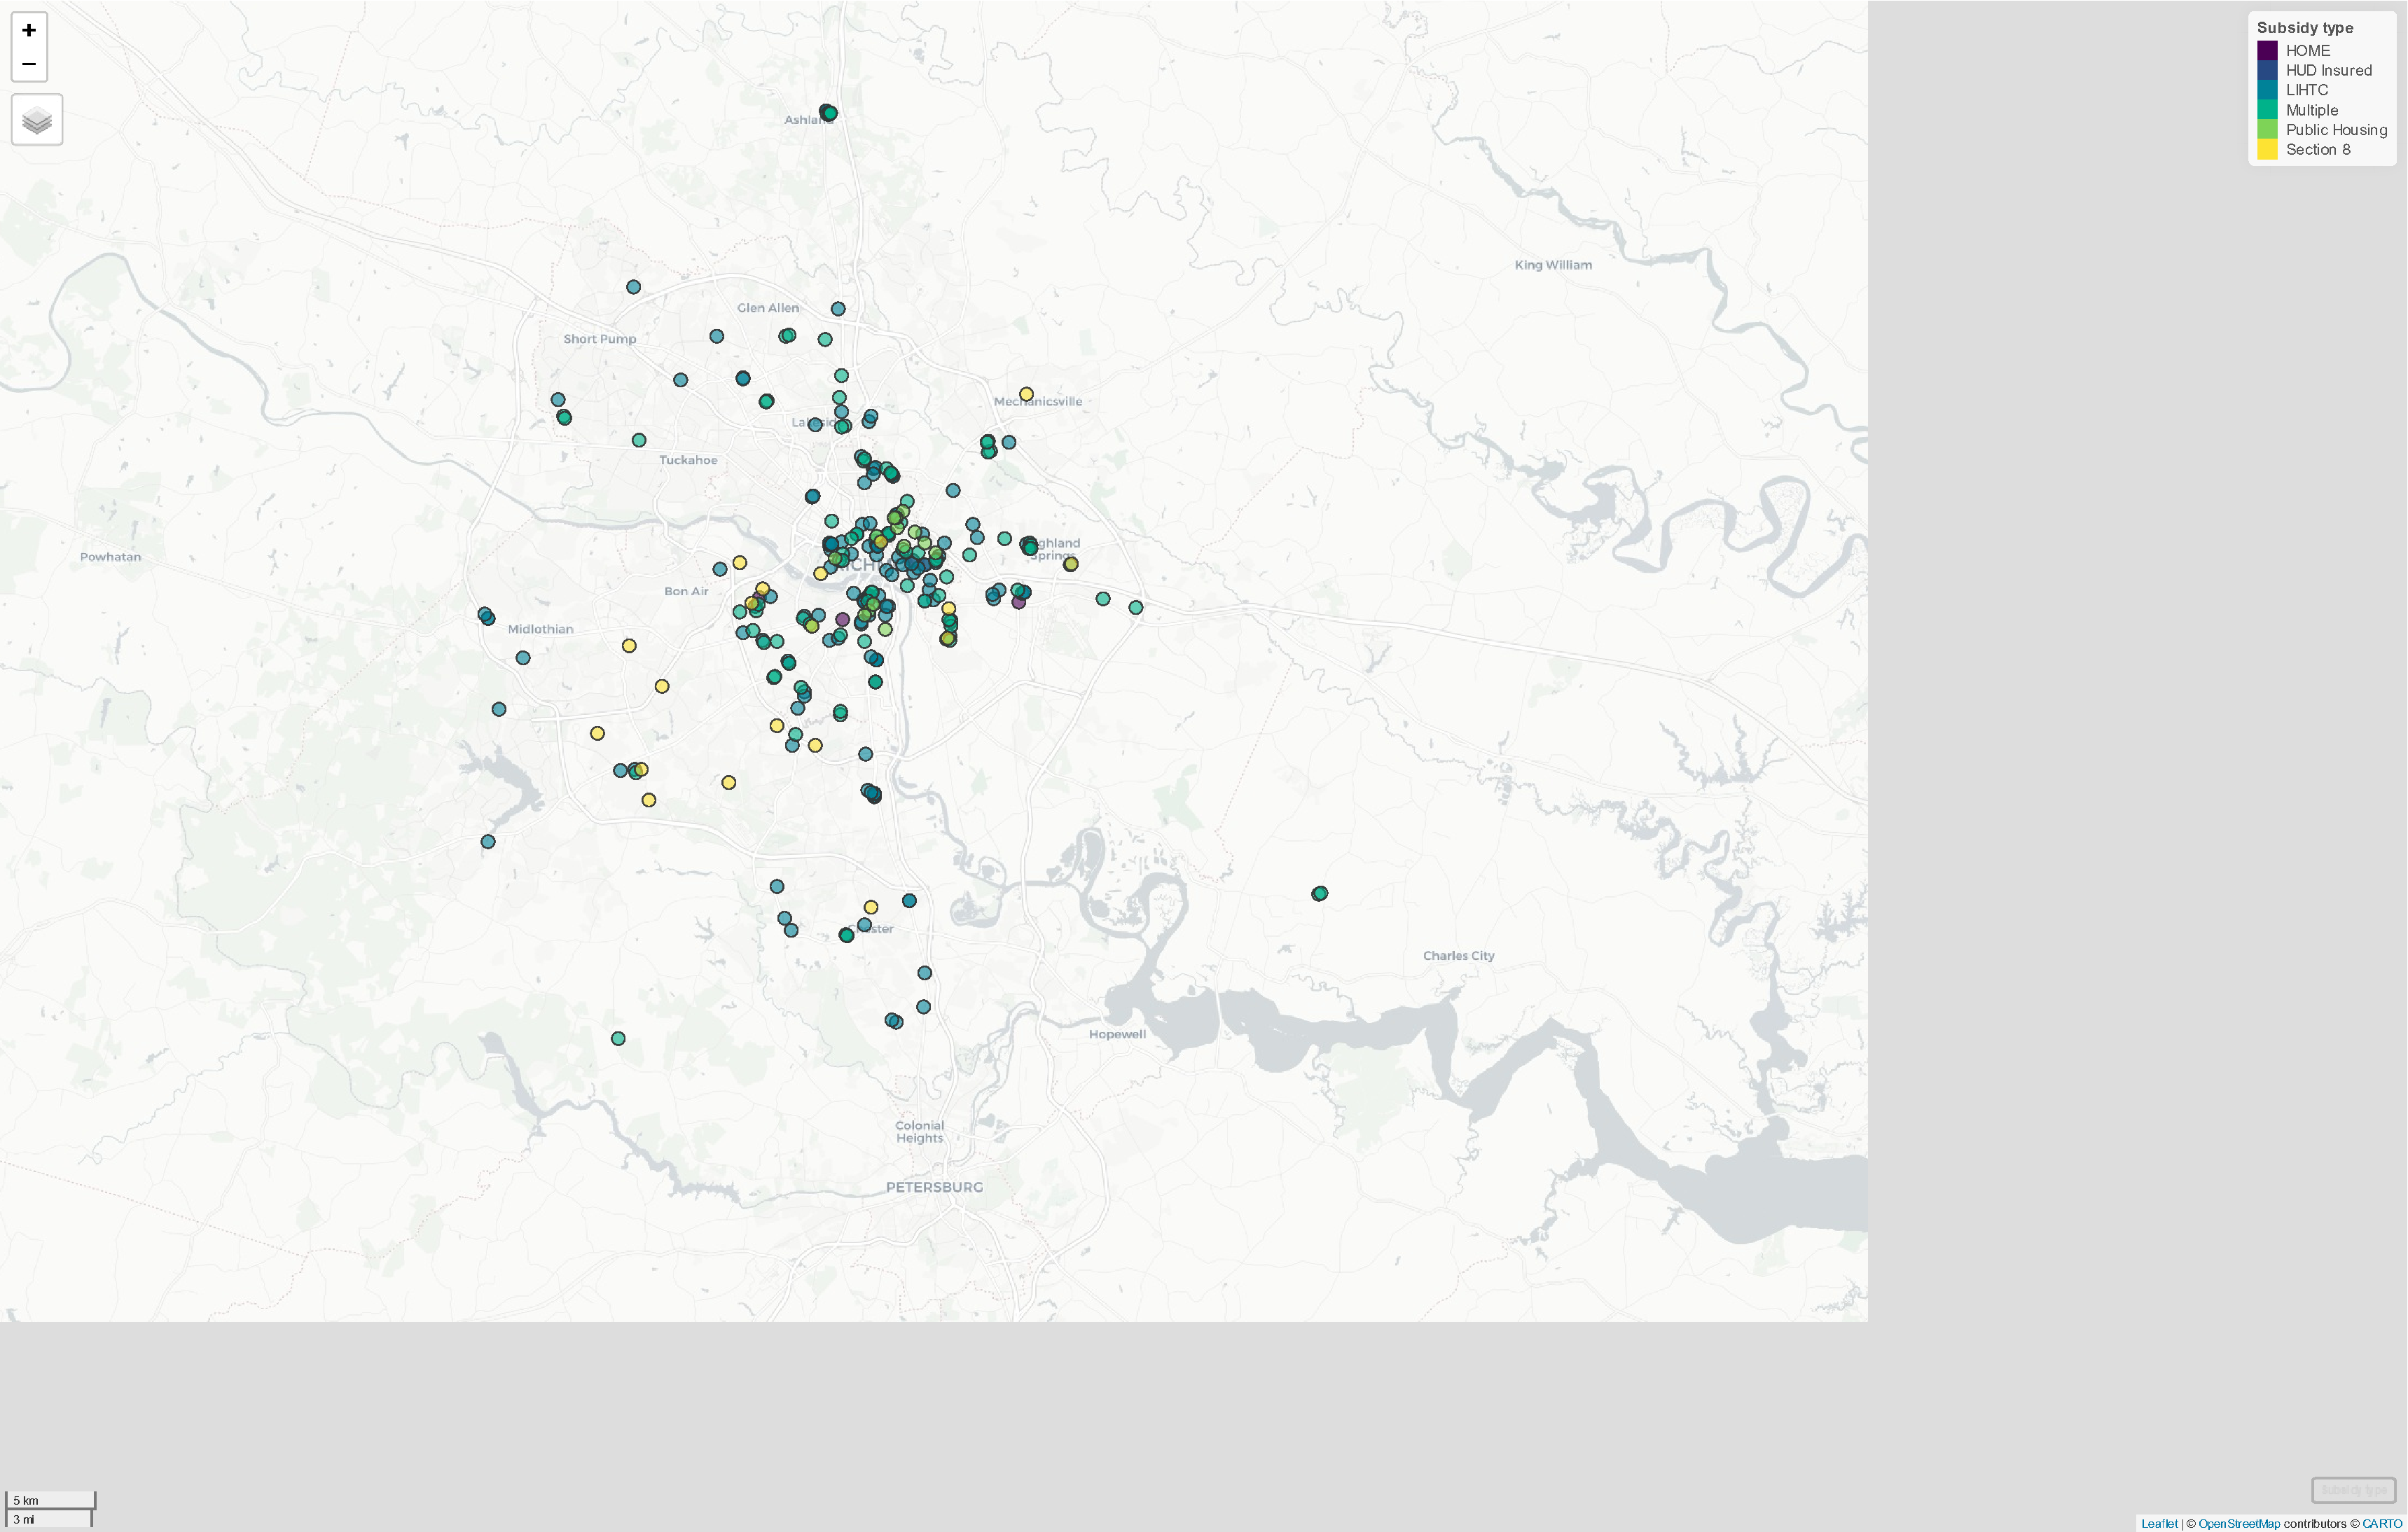
\includegraphics{./part-2-3_files/figure-pdf/fig-nhpd-map-1.pdf}

}

\caption{\label{fig-nhpd-map}Federally-assisted rental housing
properties}

\end{figure}

Richmond continues to support the majority of affordable rentals in the
region (about 60 percent---more than 15,200). While Chesterfield and
Henrico counties both have similar amounts of LIHTC-only units, Henrico
has nearly 2,900 additional units supported by multiple
subsidies---generally combinations of LIHTC and a Section 8 program.

\begin{figure}

{\centering \includegraphics{./part-2-3_files/figure-pdf/fig-subsidy-location-1.pdf}

}

\caption{\label{fig-subsidy-location}Federally assisted units by subsidy
and locality}

\end{figure}

\hypertarget{changes-since-2020}{%
\subsection{Changes since 2020}\label{changes-since-2020}}

Since January 2020, the region has seen 57 new rental subsidies added,
which increased the number of active affordability contracts on units by
4,393. Over that same period, 17 subsidies ended, affecting 1,633 units.
Some properties had multiple subsidies either added or expired. In all,
there was a net addition of 2,760 rental affordability contracts.

\hypertarget{tbl-change-table}{}
\begin{table}
\caption{\label{tbl-change-table}Added and removed affordable rental contracts since 2020 }\tabularnewline

\centering
\begin{tabular}{l|r|r|r}
\hline
 & Subsidies & Properties affected & Units included\\
\hline
Added & 57 & 53 & 4,393\\
\hline
Removed & -17 & -16 & -1,633\\
\hline
\textbf{Net change} & \textbf{40} & \textbf{37} & \textbf{2,760}\\
\hline
\multicolumn{4}{l}{\rule{0pt}{1em}Sources: National Housing Preservation Database and Virginia Housing.}\\
\end{tabular}
\end{table}

New LIHTC units (net 2,129) comprised the majority of added affordable
rentals, followed by Section 8 contracts (net 1,132). Net losses of
affordable rental contracts occurred in projects supported by HOME
funding and HUD insurance.

\begin{figure}

{\centering \includegraphics{./part-2-3_files/figure-pdf/fig-change-fig-1.pdf}

}

\caption{\label{fig-change-fig}Additions and removals of subsidized
rental units}

\end{figure}

While LIHTC additions drove new affordable supply in Richmond and
Chesterfield, new (or renewed) Section 8 contracts covered more than 400
units in Henrico. Over 500 units in Richmond and Henrico saw HUD
insurance contracts expire; however, many of these are in projects with
another form of rental assistance that has not expired.

\begin{figure}

{\centering \includegraphics{./part-2-3_files/figure-pdf/fig-change-locality-1.pdf}

}

\caption{\label{fig-change-locality}Net change in subsidized rental unit
contracts by locality}

\end{figure}

\hypertarget{lihtc-preservation}{%
\subsection{LIHTC preservation}\label{lihtc-preservation}}

LIHTC properties have a 30 year commitment to affordability, but only a
15 year compliance period, wherein property owners can increase rents.
Nonprofit developers will often seek new allocation of tax credits
before their commitment period ends, but there is often little incentive
for for-profit developers to maintain affordability restrictions past
the compliance period.

By 2040, a large portion of active LIHTC units will be outside the 30
year commitment period --- even far more will be outside the 15 year
compliance period. Just over 13,000 LIHTC units will be beyond the 30
year commitment period by 2040, which accounts for well over half of all
active LIHTC units as of early 2022.

\begin{figure}

{\centering \includegraphics{./part-2-3_files/figure-pdf/fig-lihtc-1.pdf}

}

\caption{\label{fig-lihtc}Percent of active LIHTC units by end of
commitment period}

\end{figure}

\hypertarget{public-housing}{%
\subsection{Public Housing}\label{public-housing}}

The redevelopment of public housing in the City of Richmond has begun to
take shape at the first of the ``Big Six'' public housing courts ---
\href{https://www.rrha.com/redevelopment/creighton/}{\textbf{Creighton
Court}}. This public housing property located in Richmond's far East End
consisted of 504 public housing units.

As part of their first phase of redevelopment, RRHA has begun demolition
of Creighton Court, with plans to develop roughly 700 units of
mixed-income housing. Construction on Phase 1 is expected to begin in
Winter 2022 with the entire redevelopment process expected to last ten
years.

RRHA's next focus area will be
\href{https://www.rrha.com/redevelopment/jackson-ward/}{\textbf{Gilpin
Court}}, north of Jackson Ward, where about 780 public housing units
reside. In November 2021, RRHA and the City of Richmond were awarded a
Choice Neighborhoods Planning Grant by the U.S. Department of Housing
and Urban Development for \$450,000.

This planning grant is being utilized to facilitate the community
planning process around not only Gilpin Court, but the Jackson Ward
community --- including strategies to undo the negative impacts of
interstate development on the historically Black communities of Jackson
Ward and North Jackson Ward.

\begin{longtable}[]{@{}
  >{\raggedright\arraybackslash}p{(\columnwidth - 6\tabcolsep) * \real{0.3562}}
  >{\raggedleft\arraybackslash}p{(\columnwidth - 6\tabcolsep) * \real{0.2192}}
  >{\raggedleft\arraybackslash}p{(\columnwidth - 6\tabcolsep) * \real{0.2603}}
  >{\raggedleft\arraybackslash}p{(\columnwidth - 6\tabcolsep) * \real{0.1644}}@{}}
\caption{Net change in units for public housing
redevelopment}\tabularnewline
\toprule()
\begin{minipage}[b]{\linewidth}\raggedright
Public housing community
\end{minipage} & \begin{minipage}[b]{\linewidth}\raggedleft
Original units
\end{minipage} & \begin{minipage}[b]{\linewidth}\raggedleft
Replacement units
\end{minipage} & \begin{minipage}[b]{\linewidth}\raggedleft
Net change
\end{minipage} \\
\midrule()
\endfirsthead
\toprule()
\begin{minipage}[b]{\linewidth}\raggedright
Public housing community
\end{minipage} & \begin{minipage}[b]{\linewidth}\raggedleft
Original units
\end{minipage} & \begin{minipage}[b]{\linewidth}\raggedleft
Replacement units
\end{minipage} & \begin{minipage}[b]{\linewidth}\raggedleft
Net change
\end{minipage} \\
\midrule()
\endhead
Creighton Court & 504 & 700 & +196 \\
Gilpin Court & 780 & TBD & TBD \\
\bottomrule()
\end{longtable}

\begin{tcolorbox}[enhanced jigsaw, colframe=quarto-callout-tip-color-frame, arc=.35mm, bottomrule=.15mm, colbacktitle=quarto-callout-tip-color!10!white, opacityback=0, left=2mm, rightrule=.15mm, title=\textcolor{quarto-callout-tip-color}{\faLightbulb}\hspace{0.5em}{Funding for Public Housing redevelopment}, colback=white, coltitle=black, toptitle=1mm, leftrule=.75mm, titlerule=0mm, breakable, opacitybacktitle=0.6, toprule=.15mm, bottomtitle=1mm]

Federal housing policy has guided public housing authorities to use
newer funding streams to redevelop older public housing communities. For
these efforts, RRHA and its partners will use LIHTC, Tenant Protection
Vouchers, Project-Based Vouchers, and other federal, state, and local
sources.

\end{tcolorbox}

\hypertarget{rental-assistance}{%
\section{Rental assistance}\label{rental-assistance}}

\hypertarget{housing-choice-vouchers}{%
\subsection{Housing Choice Vouchers}\label{housing-choice-vouchers}}

Section 8 Housing Choice Vouchers (HCV) are tenant-based rental
assistance that allows recipients to find housing on the open market.
This provides household with greater choice in where they want to live,
but historically many HCV recipients have faced discrimination from
landlords unwilling to accept HCV.

This changed significantly in early 2020, when the Virginia General
Assembly passed
\href{https://homeofva.org/get-help/fair-housing/source-of-funds/}{new
fair housing legislation} that made it illegal to discriminate based on
source of income --- defined as:

\begin{quote}
\emph{``any source that lawfully provides funds to or on behalf of a
renter or buyer of housing, including any assistance, benefit, or
subsidy program, whether such program is administered by a governmental
or nongovernmental entity.''}
\end{quote}

HCV utilization across the region is concentrated in the East End and
Southside of Richmond, but can also be found throughout the counties, as
well as the Town of Ashland. Higher HCV utilization (above 20 percent)
is seen in areas near Fulton Hill, Oakwood, Manchester, and Bellwood in
Chesterfield County.

\begin{figure}

{\centering \includegraphics{./part-2-3_files/figure-pdf/fig-hcv-1.pdf}

}

\caption{\label{fig-hcv}Percent of renters with Housing Choice Vouchers
by tract}

\end{figure}

\hypertarget{rent-relief-and-mortgage-relief}{%
\subsection{Rent relief and mortgage
relief}\label{rent-relief-and-mortgage-relief}}

In response to the COVID-19 pandemic's impact on renters across the
nation, Congress created a \$25 billion Emergency Rental Assistance
(ERA) program that was funded through the CARES Act in 2021. The program
was implemented through the U.S. Treasury Department and resulted in a
total of \$1 billion being allocated to the Commonwealth of Virginia and
eligible local governments.

With this funding, the Virginia Department of Housing and Community
Development (DHCD) established the Virginia Rent Relief Program (RRP),
while Chesterfield County elected to administer their own rental
assistance program through local nonprofit, Area Congregations Together
in Service (ACTS).

Through DHCD, a total of 32,029 payments were made to households across
Richmond, Henrico, and Hanover. Both Richmond and Henrico saw increasing
households receiving rental assistance with slight dips during the early
part of 2022. Few households in Hanover County sought rental relief from
DHCD.

\begin{tcolorbox}[enhanced jigsaw, colframe=quarto-callout-warning-color-frame, arc=.35mm, bottomrule=.15mm, colbacktitle=quarto-callout-warning-color!10!white, opacityback=0, left=2mm, rightrule=.15mm, title=\textcolor{quarto-callout-warning-color}{\faExclamationTriangle}\hspace{0.5em}{All data not available}, colback=white, coltitle=black, toptitle=1mm, leftrule=.75mm, titlerule=0mm, breakable, opacitybacktitle=0.6, toprule=.15mm, bottomtitle=1mm]

Chesterfield County rent relief data has not been received yet.

\end{tcolorbox}

\begin{figure}

{\centering \includegraphics{./part-2-3_files/figure-pdf/fig-rrp-1.pdf}

}

\caption{\label{fig-rrp}Rent relief payments by locality}

\end{figure}

Average payments per household across the three localities was well
above \$4,000 for most of the program's duration, with the highest
payments being made in Hanover County.

\begin{figure}

{\centering \includegraphics{./part-2-3_files/figure-pdf/fig-rrp-payment-1.pdf}

}

\caption{\label{fig-rrp-payment}Average assistance by month and
locality}

\end{figure}

\hypertarget{affordable-homeownership}{%
\section{Affordable homeownership}\label{affordable-homeownership}}

Since 2018, nonprofit developers in the region have averaged about 53
affordable homes sold to low-income buyers a year. Most of this
production is attributable to Southside Community Development and
project:HOMES.

\begin{figure}

{\centering \includegraphics{./part-2-3_files/figure-pdf/fig-pha-homeownership-1.pdf}

}

\caption{\label{fig-pha-homeownership}Richmond region nonprofit
homeownership production}

\end{figure}

\hypertarget{part-2-4}{%
\chapter{Assessment of naturally-occurring affordable
housing}\label{part-2-4}}

This chapter covers trends in naturally-occurring affordable housing
(NOAH), or market affordable housing.

\hypertarget{naturally-occurring-affordable-housing}{%
\section{Naturally-occurring affordable
housing}\label{naturally-occurring-affordable-housing}}

Not all affordable housing is supported by public subsidy. In fact, a
large share of affordable housing is privately-owned and receives no
government assistance. Widely referred to as
\href{https://www.mckinsey.com/industries/public-and-social-sector/our-insights/preserving-the-largest-and-most-at-risk-supply-of-affordable-housing}{naturally
occurring affordable housing (NOAH)}, or market-affordable housing,
these properties are a growing concern for communities facing housing
affordability challenges.

\begin{tcolorbox}[enhanced jigsaw, colframe=quarto-callout-note-color-frame, arc=.35mm, bottomrule=.15mm, colbacktitle=quarto-callout-note-color!10!white, opacityback=0, left=2mm, rightrule=.15mm, title=\textcolor{quarto-callout-note-color}{\faInfo}\hspace{0.5em}{Is it really ``naturally-occurring''?}, colback=white, coltitle=black, toptitle=1mm, leftrule=.75mm, titlerule=0mm, breakable, opacitybacktitle=0.6, toprule=.15mm, bottomtitle=1mm]

Many experts consider NOAH to be a
\href{https://cityobservatory.org/the-myth-of-naturally-occurring-affordable-housing/}{misnomer}
because there is nothing ``natural'' about the affordability of these
properties. Some prefer
\href{https://www.allianceforhousingsolutions.org/market-rate-affordable-housing}{``market-rate
affordable''}. But regardless of the choice of term, this type of
housing plays a pivotal, albeit precarious, role in providing localities
with a significant amount of affordable housing without government
resources.

\end{tcolorbox}

The preservation of NOAH properties has been a growing strategy to
support affordable housing in communities as the ability to quickly
develop new units has been stifled by labor shortages, rising land
prices, and supply chain issues. NOAH is at great risk of being lost
because it often requires greater investment to maintain and more likely
to be redeveloped---in turn contributing to a loss of affordable housing
units.

\begin{tcolorbox}[enhanced jigsaw, colframe=quarto-callout-note-color-frame, arc=.35mm, bottomrule=.15mm, colbacktitle=quarto-callout-note-color!10!white, opacityback=0, left=2mm, rightrule=.15mm, title=\textcolor{quarto-callout-note-color}{\faInfo}\hspace{0.5em}{Defining NOAH}, colback=white, coltitle=black, toptitle=1mm, leftrule=.75mm, titlerule=0mm, breakable, opacitybacktitle=0.6, toprule=.15mm, bottomtitle=1mm]

For analysis purposes, we define NOAH properties as:

\begin{itemize}
\tightlist
\item
  Existing multifamily properties with active leases;
\item
  Classified as Class B, C, or unclassified;
\item
  No public subsidy, rent caps, or other income-based restrictions;
\item
  \emph{CoStar Building Rating} of two or fewer stars out of
  five;\footnote{Per CoStar, this is rating for the building relative to
    other buildings of the same type throughout the country.} and
\item
  Built before 2000
\end{itemize}

\end{tcolorbox}

\hypertarget{locations-1}{%
\subsection{Locations}\label{locations-1}}

Based on this criteria, NOAH properties are located all across the
region, especially in the City of Richmond and along the borders of the
city and counties, where older multifamily properties exist.

\begin{figure}

{\centering \includegraphics{./part-2-4_files/figure-pdf/fig-noah-map-1.pdf}

}

\caption{\label{fig-noah-map}NOAH properties in Richmond region}

\end{figure}

The large share of NOAH is located in the City of Richmond (11,253 units
or 45 percent of all NOAH units). This is no doubt due to the large
amount of older multifamily properties within city limits --- most of
which is located in smaller buildings. Henrico County has the second
largest share of NOAH in the region with 8,983 units, followed by
Chesterfield County at 3,667 and Hanover County below 500 units.

\begin{tcolorbox}[enhanced jigsaw, colframe=quarto-callout-caution-color-frame, arc=.35mm, bottomrule=.15mm, colbacktitle=quarto-callout-caution-color!10!white, opacityback=0, left=2mm, rightrule=.15mm, title=\textcolor{quarto-callout-caution-color}{\faFire}\hspace{0.5em}{Danger}, colback=white, coltitle=black, toptitle=1mm, leftrule=.75mm, titlerule=0mm, breakable, opacitybacktitle=0.6, toprule=.15mm, bottomtitle=1mm]

It is important to consider that the City of Richmond contains much of
the region's older housing stock. This includes many older apartment
buildings that are anywhere from two to twenty units in size. While they
may fall under the NOAH classification set out in this analysis, their
rents may actually be higher due to the overwhelming demand for rental
housing among young professionals and students in the city.

Comparably cheaper than new multifamily properties that offer amenities
such as pools and fitness centers, these properties are still able to
command such high rents due to their proximity to Virginia Commonwealth
University and Virginia Union University, as well as other urban
amenities like restaurants, bars, and retail.

\end{tcolorbox}

In total, there are nearly 25,000 NOAH units across 194 properties in
the region. This makes up a significant amount of rental inventory, as
well as a valuable source of unsubsidized affordable housing. The aging
of these properties, as well as the increasing demand for rental
housing, puts significant pressure on these properties and their owners.
For smaller landlords, the cost to renovate can be far too great ---
leading to worsening deferred maintenance and pressure to sell, which
both can negatively impact renters.

\begin{figure}

{\centering \includegraphics{./part-2-4_files/figure-pdf/fig-noah-cnt-1.pdf}

}

\caption{\label{fig-noah-cnt}NOAH units by locality}

\end{figure}

\hypertarget{building-style}{%
\subsection{Building style}\label{building-style}}

CoStar places buildings into style categories based on the following
definitions:

\begin{longtable}[]{@{}lll@{}}
\toprule()
Style & Stories & Buildings \\
\midrule()
\endhead
Garden & 1-3 Stories & 4 or more buildings \\
Low-Rise & 1-3 Stories & 1-3 buildings \\
Mid-Rise & 4-14 Stories & 1 or more buildings \\
High Rise & 15+ Stories & 1 or more buildings \\
\bottomrule()
\end{longtable}

While not traditional multifamily properties, CoStar does track some
single-family and townhome rentals that are included in this data.

Roughly four out of five NOAH units are part of garden style properties,
which are clusters of smaller one- to three-story buildings. Another
3,200 units in low-rise properties, which have similar but fewer
buildings per community, round out nearly all of the NOAH supply in the
region.

However, garden style properties have more than 210 units on average,
while low-rise properties have just 12. As a result, there more than
twice as many low-rise properties (273) than garden properties (95).

\begin{figure}

{\centering \includegraphics{./part-2-4_files/figure-pdf/fig-noah-style-1.pdf}

}

\caption{\label{fig-noah-style}NOAH units and properties by building
style}

\end{figure}

The map below shows NOAH properties by building style across the region.
Most of the low-rise properties are within Richmond, reflecting the
early 20th century small-scale apartment buildings found across many
historic neighborhoods in the city---especially the Fan and Museum
District.

Garden style properties, on the other hand, are more commonly found in
the counties' inner suburbs, and reflect development trends prevalent
during those areas' growth in the mid 20th century.

\begin{figure}

{\centering \includegraphics{./part-2-4_files/figure-pdf/fig-noah-style-map-1.pdf}

}

\caption{\label{fig-noah-style-map}NOAH properties by building style}

\end{figure}

\hypertarget{age}{%
\subsection{Age}\label{age}}

With the exception of Richmond's low-rise apartments from the 1910s to
1930s, most of the region's NOAH units were built between 1960 and 1980.
CoStar also tracks property renovations, which began for NOAH properties
in the 2000s, especially closer to 2020 in Richmond and Chesterfield.

\begin{tcolorbox}[enhanced jigsaw, colframe=quarto-callout-tip-color-frame, arc=.35mm, bottomrule=.15mm, colbacktitle=quarto-callout-tip-color!10!white, opacityback=0, left=2mm, rightrule=.15mm, title=\textcolor{quarto-callout-tip-color}{\faLightbulb}\hspace{0.5em}{Substantial versus minor renovations}, colback=white, coltitle=black, toptitle=1mm, leftrule=.75mm, titlerule=0mm, breakable, opacitybacktitle=0.6, toprule=.15mm, bottomtitle=1mm]

CoStar only marks a property as renovated if it:

``\ldots{}\emph{has been completely restored so that the existing space
becomes `new' space again. {[}\ldots{]} Minor renovations, such as the
improvement of a building's lobby or exterior are not considered full
building renovations.}''

\end{tcolorbox}

\begin{figure}

{\centering \includegraphics{./part-2-4_files/figure-pdf/fig-noah-age-1.pdf}

}

\caption{\label{fig-noah-age}NOAH properties by year built}

\end{figure}

\hypertarget{rents}{%
\subsection{Rents}\label{rents}}

NOAH properties have not been immune from the rapid rises in rent. As of
Q3 2022, the average asking rent for NOAH properties was \$1,173. This
is about \$200 less than the average asking rent across all rental
properties. Although this seems like a small difference, an extra \$200
a month means more money saved for childcare or transportation costs.

From the beginning of the pandemic to Q3 2022, NOAH rent has increased
by \$104 --- a 10 percent increase.

\begin{figure}

{\centering \includegraphics{./part-2-4_files/figure-pdf/fig-noah-rents-1.pdf}

}

\caption{\label{fig-noah-rents}Average asking rent for market-affordable
multifamily}

\end{figure}

\hypertarget{sales}{%
\subsection{Sales}\label{sales}}

The sale of NOAH properties and ensuing new ownership often leads to
rent increases and/or rehabilitation. In some cases, this may take NOAH
properties out of market affordability. Over the last five years, NOAH
properties have made up well over half of all multifamily property
transactions in the region.

\begin{figure}

{\centering \includegraphics{./part-2-4_files/figure-pdf/fig-noah-sales-1.pdf}

}

\caption{\label{fig-noah-sales}Number of multifamily properties sold}

\end{figure}

However, NOAH transactions represent a smaller share of total units
sold---about one-third since 2017 Q3.

\begin{figure}

{\centering \includegraphics{./part-2-4_files/figure-pdf/fig-noah-sales-units-1.pdf}

}

\caption{\label{fig-noah-sales-units}Number of multifamily units sold}

\end{figure}

Sales volume for NOAH properties has, on average, been a small fraction
of total volume in the region. However, beginning in 2021 Q4, NOAH sales
volume rose above \$100 million for the first time since 2018 Q3, which
itself was an an outlier. NOAH sales volume hit a new record in 2022 Q1
(over \$178 million), stayed at that level the next quarter, and
continues to be well above average to-date in 2022 Q3.

\begin{figure}

{\centering \includegraphics{./part-2-4_files/figure-pdf/fig-noah-sales-vol-1.pdf}

}

\caption{\label{fig-noah-sales-vol}Volume of multifamily sales}

\end{figure}

During this timeframe, NOAH properties had an average price per unit
below that of all multifamily sales until 2020 Q4. At the end of 2020,
the average price per unit of a NOAH property hit a high of \$221,534
--- over \$44,000 more when compared to all multifamily sales. Although
both types of sales took a dip following the end of 2020, the higher
NOAH price remained until 2021 Q2, when NOAH average price per unit once
again went below all sales.

\begin{figure}

{\centering \includegraphics{./part-2-4_files/figure-pdf/fig-noah-price-unit-1.pdf}

}

\caption{\label{fig-noah-price-unit}Average price per unit}

\end{figure}

\hypertarget{manufactured-home-communities}{%
\section{Manufactured home
communities}\label{manufactured-home-communities}}

Manufactured home communities (MHCs) are also a valuable source of NOAH
across the region, but are not reliably monitors as traditional
multifamily rental housing. As a result, accurate data on supply and
rents are more difficult to obtain.

\hypertarget{supply-3}{%
\subsection{Supply}\label{supply-3}}

In 2016, the Manufactured Home Community Coalition of Virginia (MHCCV)
conducted an assessment of all manufactured home communities across the
Richmond, Virginia Metropolitan Statistical Area (MSA). That report
found 4,735 homes across 54 MHCs in the greater region. Within the
primary PHA area\footnote{Chesterfield, Hanover, Henrico, and Richmond.}
there are 24 different MHCs, which in all contained at least 2,742
individual manufactured homes.

\begin{tcolorbox}[enhanced jigsaw, colframe=quarto-callout-note-color-frame, arc=.35mm, bottomrule=.15mm, colbacktitle=quarto-callout-note-color!10!white, opacityback=0, left=2mm, rightrule=.15mm, title=\textcolor{quarto-callout-note-color}{\faInfo}\hspace{0.5em}{Note}, colback=white, coltitle=black, toptitle=1mm, leftrule=.75mm, titlerule=0mm, breakable, opacitybacktitle=0.6, toprule=.15mm, bottomtitle=1mm]

This data includes homes that may be rented, as well as owned.
Regardless, residents in MHCs rent the lot on which their home resides.
This leaves many manufactured home community residents who own their
homes in a precarious position should a community owner decide to sell
or redevelop the property. Manufactured homes are not easily moved once
installed, leaving many families forced to abandon their homes and seek
new and more expensive housing elsewhere.

\end{tcolorbox}

\begin{figure}

{\centering \includegraphics{./part-2-4_files/figure-pdf/fig-mhc-supply-1.pdf}

}

\caption{\label{fig-mhc-supply}Units in manufactured home communities by
locality}

\end{figure}

Chesterfield County has the largest supply of homes in MHCs (1,543),
which is about half the total number of subsidized rentals also in the
county. Hanover and Richmond both have near 500 units in MHCs, while
Henrico only has one MHC with 230 units.

\hypertarget{locations-2}{%
\subsection{Locations}\label{locations-2}}

The majority of manufactured home community units are located along the
Route 1 corridor. In areas where commercial and mixed-use development
has accelerated, many of these properties are well-positioned for a
change to a ``higher and better'' use. This redevelopment potential,
while often in line with broader planning goals, is a threat to the
long-term stability of MHCs.

\begin{figure}

{\centering \includegraphics{./part-2-4_files/figure-pdf/fig-mhc-map-1.pdf}

}

\caption{\label{fig-mhc-map}Manufactured housing communities in Richmond
region}

\end{figure}

\begin{tcolorbox}[enhanced jigsaw, colframe=quarto-callout-tip-color-frame, arc=.35mm, bottomrule=.15mm, colbacktitle=quarto-callout-tip-color!10!white, opacityback=0, left=2mm, rightrule=.15mm, title=\textcolor{quarto-callout-tip-color}{\faLightbulb}\hspace{0.5em}{Notable changes since 2020}, colback=white, coltitle=black, toptitle=1mm, leftrule=.75mm, titlerule=0mm, breakable, opacitybacktitle=0.6, toprule=.15mm, bottomtitle=1mm]

In September 2020, project:HOMES,
\href{https://www.projecthomes.org/bermuda-estates}{acquired} a 52 unit
manufactured home community called Bermuda Estates in Chesterfield
County. Since acquiring the community, project:HOMES has made
significant infrastructure improvements, replaced some units in
disrepair, and constructed a community center. The nonprofit plans to
continue investments and preserve the park as a high-quality, low-cost
neighborhood.

Suburban Village, Chesterfield County's third largest MHC with almost
250 units, was
\href{https://richmond.com/news/local/maryland-based-investment-firm-buys-chesterfield-mobile-home-park-for-22-5-million/article_41bd2656-0466-5643-9285-2715e88fee40.html}{purchased}
by Maryland-based Horizon Land Management in August 2021 for \$22.5
million. The park was previously under the same local ownership since
1986. More than 35 potential buyers expressed interest.

Shady Hill Mobile Home Park, home to more than 100 families, was
purchased by a Charlottesville-based development firm for \$5.1 million
in August 2022. While complete redevelopment is likely, exact plans and
timing are not known.

\end{tcolorbox}

\part{PART 3: Gap analysis}

\hypertarget{part-3-1}{%
\chapter{Affordability of current housing supply}\label{part-3-1}}

This chapter is an analysis of existing housing costs versus the ability
of households in the region to afford those housing costs.

\hypertarget{rental-housing-gap}{%
\section{Rental housing gap}\label{rental-housing-gap}}

\href{https://www.huduser.gov/portal/datasets/cp.html}{Comprehensive
Housing Affordability Strategy (CHAS)} data provided by the Department
of Housing and Urban Development (HUD) allows us to understand the cost
of housing in relation to household incomes. For renters making less
than 80\% AMI across the region, there has been little change in the gap
in affordable rental housing.

\begin{figure}

{\centering \includegraphics{./part-3-1_files/figure-pdf/fig-gap-plot-1.pdf}

}

\caption{\label{fig-gap-plot}Rental housing gap by AMI}

\end{figure}

In 2015, there was an overall gap of 38,778 rental homes affordable to
households making 80\% AMI or less. By 2019, that gap had increased by
1,220 homes to reach a total gap of 38,778.

Increases in the gap occurred mainly among housing at 30 percent AMI and
below, but it is important to note that a gap in housing across all
income levels impacts households of any income. This accentuates the
need for new affordable housing at all income levels --- but especially
for 30\% AMI or below households. As of 2018, these extremely low-income
renters face a shortage of over 24,000 rental homes.

\hypertarget{incomes-versus-housing-costs}{%
\section{Incomes versus housing
costs}\label{incomes-versus-housing-costs}}

\hypertarget{overview}{%
\subsection{Overview}\label{overview}}

Housing costs---both for-sale prices and rents---have steadily
accelerated in the region since 2016. Every locality say home prices
rise more than 50 percent, with average rents not far behind. Average
renter incomes also increased from 2016 to 2020, although those gains
were not as steady across all localities.

\begin{figure}

{\centering \includegraphics{./part-3-1_files/figure-pdf/fig-costs-inc-change-1.pdf}

}

\caption{\label{fig-costs-inc-change}Cumulative percent change in median
renter income, home prices, and average rent}

\end{figure}

However, there are two other important takeaways:

\begin{enumerate}
\def\labelenumi{\arabic{enumi}.}
\tightlist
\item
  Average renter income data is currently only available through 2020,
  while the sharpest housing price increases occurred from then through
  2022.
\item
  Average renter incomes were already below the level necessary to
  afford the typical apartment or home for sale.
\end{enumerate}

\hypertarget{rental-affordability}{%
\subsection{Rental affordability}\label{rental-affordability}}

Market asking rents across the region have been on the incline between
2016. Still, the median incomes for renters in Chesterfield and
Henrico---at least from 2016 to 2020---could afford average rents. That
was not the case for Henrico and Richmond, where the monthly rental
price affordability gaps were \$20 and \$218, respectively.

\begin{tcolorbox}[enhanced jigsaw, colframe=quarto-callout-tip-color-frame, arc=.35mm, bottomrule=.15mm, colbacktitle=quarto-callout-tip-color!10!white, opacityback=0, left=2mm, rightrule=.15mm, title=\textcolor{quarto-callout-tip-color}{\faLightbulb}\hspace{0.5em}{Calculating rental affordability}, colback=white, coltitle=black, toptitle=1mm, leftrule=.75mm, titlerule=0mm, breakable, opacitybacktitle=0.6, toprule=.15mm, bottomtitle=1mm]

In this chapter, an ``affordable rent'' is no more than 30 percent of a
household's gross monthly income. Any rent amount higher than this level
would make the renter cost-burdened.

\end{tcolorbox}

\begin{figure}

{\centering \includegraphics{./part-3-1_files/figure-pdf/fig-rent-afford-1.pdf}

}

\caption{\label{fig-rent-afford}Average rents versus affordable rents
for median renter income}

\end{figure}

\hypertarget{homeownership-affordability}{%
\subsection{Homeownership
affordability}\label{homeownership-affordability}}

To determine how affordable homeownership is at the median renter
income, we can calculate the maximum home sales price affordable to a
buyer with that income. To make these estimates, we make the following
simplified assumptions:

\begin{itemize}
\tightlist
\item
  5 percent down payment
\item
  1.5 percent in closing costs
\item
  \$250 per month for property taxes
\item
  \$150 per month for insurance and other costs
\end{itemize}

For underwriting purposes, we assume that the monthly mortgage payment
plus these costs can not exceed 28 percent of the buyer's gross income.
For example, a renter earning \$50,000 can afford a monthly housing cost
no more than \$1,166.67.

To determine the maximum principal amount, and the subsequent sales
price, we assume a standard 30-year fixed-rate mortgage using the
average annual interest rates published by Freddie Mac\footnote{Freddie
  Mac, \href{https://www.freddiemac.com/pmms/pmms30}{30-Year Fixed-Rate
  Mortgages Since 1971}.}. The 2022 value is the average through August.
The figure below shows these interest rates used for the homeowner
affordability analysis.

\begin{figure}

{\centering \includegraphics{./part-3-1_files/figure-pdf/fig-int-rates-1.pdf}

}

\caption{\label{fig-int-rates}Average annual rates for 30-year
fixed-rate mortgages}

\end{figure}

The figure below shows these maximum affordable home sales prices versus
actual median sales prices for each locality from 2016 through 2020.
Only median sales prices are shown for 2021 and 2022 year-to-date, since
renter income estimates from ACS are only available through 2020.

\begin{figure}

{\centering \includegraphics{./part-3-1_files/figure-pdf/fig-price-afford-1.pdf}

}

\caption{\label{fig-price-afford}Median sales price versus maximum home
price affordable to median renter income}

\end{figure}

In the three counties, median sales prices were generally just out of
reach for the average renter's income from 2016 through 2019. Then,
historically low interest rates in 2020 increased buyers' purchasing
power to put the median-priced home within reach.

The purchase price gap in Richmond, however, has continued---even with
lower rates, the average renter could not afford to buy a home more than
\$200,000 in 2020. By 2021, the median-priced home in the city topped
\$300,000 for the first time.

\hypertarget{wage-based-affordability}{%
\section{Wage-based affordability}\label{wage-based-affordability}}

In a \protect\hyperlink{wages}{previous chapter}, the five most common
occupation categories in the Richmond MSA were determined from the
latest (May 2021) BLS Occupational Employment and Wage Statistics (OEWS)
data. These wages are an opportunity to assess the ability of many of
the region's workers to afford rent or purchase a home. Annual salary
amounts range from \$75,800 for workers in Business and Financial
Operations, to \$23,650 for those in Food Preparation and Serving
Related positions.

\begin{figure}

{\centering \includegraphics{./part-3-1_files/figure-pdf/fig-occ-salary-1.pdf}

}

\caption{\label{fig-occ-salary}Median annual salaries for the five most
common occupation categories}

\end{figure}

\hypertarget{rental-affordability-1}{%
\subsection{Rental affordability}\label{rental-affordability-1}}

Every occupation except for Business and Financial Operations supports
an affordable rent less than \$1,000. Apartments in the region for less
than this are hard to come by, and average rents across localities are
now hundreds of dollars more.

\begin{figure}

{\centering \includegraphics{./part-3-1_files/figure-pdf/fig-occ-rent-1.pdf}

}

\caption{\label{fig-occ-rent}Affordable rent by occupation versus
average rents}

\end{figure}

However, these average rents \emph{can} be relatively attainable if
households have two earners with annual salaries each above \$30,000.
Still, even dual-income households where both workers are in retail
and/or restaurant jobs would currently struggle to find an affordable
apartment anywhere in the region.

\hypertarget{homeownership-affordability-1}{%
\subsection{Homeownership
affordability}\label{homeownership-affordability-1}}

Similarly, all occupation categories other than Business and Financial
Operations command wages that make homeownership a challenging goal,
especially for single-earner households. Most of these common jobs, on
their own, would support only home purchases prices below \$140,000.
This does not even consider related financial barriers often faced by
lower-income workers, such as savings for down payments and acceptable
credit scores.

\begin{figure}

{\centering \includegraphics{./part-3-1_files/figure-pdf/fig-occ-price-1.pdf}

}

\caption{\label{fig-occ-price}Maximum affordable home price by
occupation versus median sales prices}

\end{figure}

\hypertarget{part-3-2}{%
\chapter{Impact of housing costs on household budgets}\label{part-3-2}}

\hypertarget{cost-burden}{%
\section{Cost burden}\label{cost-burden}}

When incomes don't rise along with housing costs, we can expect an
increase in the number of cost-burdened households who pay more than 30
percent of their gross income on basic housing expenses. Since 2015,
cost burden levels in the region decreased for some groups, while
increased for others.

Data in this section come from the Comprehensive Housing Affordability
Strategy (CHAS) dataset published by the U.S. Department of Housing and
Urban Development. CHAS estimates are a custom tabulation of American
Community Survey responses. As of October 2022, the most recent CHAS
data is for the 2015-2019 5-year period.

Unless otherwise noted, all plots on this page combine data from
Chesterfield County, Hanover County, Henrico County, and Richmond city.

\hypertarget{cost-burden-by-tenure}{%
\subsection{Cost burden by tenure}\label{cost-burden-by-tenure}}

The number of cost-burdened homeowners across the region has declined
significantly since 2015, particularly in Chesterfield and Henrico
counties. Hanover County and Richmond city saw smaller decreases, but
the total ``loss'' of cost-burdened homeowners in the region still
exceeded 7,200.

Meanwhile, the total number of cost-burdened renter households increased
by almost 1,900, with only Hanover County seeing a small decline. Much
of this growth in renter cost burden was focused in Chesterfield County
and Richmond city.

\begin{figure}

{\centering \includegraphics{./part-3-2_files/figure-pdf/fig-cb-locality-1.pdf}

}

\caption{\label{fig-cb-locality}Cumulative change in cost-burdened
households by tenure}

\end{figure}

\hypertarget{cost-burden-by-income}{%
\subsection{Cost burden by income}\label{cost-burden-by-income}}

Homeowners above 80 percent AMI saw the largest declines in cost burden
since 2015. This is likely due to rising incomes among homeowners with
relatively fixed housing costs. Although renters with higher incomes
were seeing growing cost burden from 2015 to 2018, 2019 estimates show
an abrupt shift in trends. Renters making less than 50 percent AMI saw
an increase in cost burden from 2015 of nearly 4,000 households. The
number of households making greater than 50 percent AMI saw an overall
decrease in cost burden from 2015 estimates --- reversing the increases
seen in 2018.

\begin{figure}

{\centering \includegraphics{./part-3-2_files/figure-pdf/fig-cb-income-1.pdf}

}

\caption{\label{fig-cb-income}Cumulative change in cost-burdened
households by income and tenure}

\end{figure}

However, the significant and unexpected drop among cost-burdened renters
below 30 percent AMI from 2017 to 2018 deserves further explanation. The
increase in 2019 appears to be more aligned with our sense of the rental
housing market over the past few years.

The plot below shows the ACS estimates of renter households by cost
burden from 2016 to 2020. There is a steady decline in the number of
cost-burdened low-income renters (under \$35,000); however, this
corresponds to an increasing number of cost-burdened renters with
incomes between \$35,000 and \$75,000.

\begin{figure}

{\centering \includegraphics{./part-3-2_files/figure-pdf/fig-cb-income-acs-est-1.pdf}

}

\caption{\label{fig-cb-income-acs-est}Renter households by income and
cost burden}

\end{figure}

Nearly all cost-burdened renter households have incomes below \$75,000.
Filtering for just those estimates, the plot below shows the net annual
change from 2016 to 2020. The significant decrease from 2019 to 2020
(1,057) is well beyond the range from previous changes, and may also be
due in part to lower ACS response rates among lower-income households
during the COVID-19 pandemic.

\begin{figure}

{\centering \includegraphics{./part-3-2_files/figure-pdf/fig-cb-income-acs-yoy-1.pdf}

}

\caption{\label{fig-cb-income-acs-yoy}Year-over-year change in
cost-burdened renter households}

\end{figure}

In summary, since the \emph{total} number of renter households in the
region has not changed significantly from 2016 to 2020, and because the
supply of deeply affordable rental housing has not increased, the
estimated decline in low-income cost-burdened renters is likely due to a
combination of increasing average incomes ``re-sorting'' households into
higher income categories, as well as pandemic data collection
challenges.

\hypertarget{cost-burden-by-household-type}{%
\subsection{Cost burden by household
type}\label{cost-burden-by-household-type}}

Small families and non-elderly, non-family homeowner households saw the
largest decreases in cost burden across all four localities. Among
renters, only small family households are now less likely to be
cost-burdened, but this change (-765) is an order of magnitude smaller
than the decrease for homeowner small families (-6,525).

Net increases in cost-burden were almost entirely contained to elderly
non-family and elderly family households. There are now more than 4,600
additional cost-burdened households in these groups, including both
homeowners and renters.

\begin{figure}

{\centering \includegraphics{./part-3-2_files/figure-pdf/fig-cb-hh-1.pdf}

}

\caption{\label{fig-cb-hh}Change in cost-burdened households by
household type}

\end{figure}

\hypertarget{mortgage-delinquency-and-foreclosure}{%
\section{Mortgage delinquency and
foreclosure}\label{mortgage-delinquency-and-foreclosure}}

Since the Great Recession, mortgage delinquency of 90 days or more has
been on a steady decline across the region ---reaching the decade's
lowest rates throughout much of 2020 and 2021. Pandemic mortgage relief
measures laid out in the CARES Act led to a significant forbearance
program, wherein homeowners with federally-backed mortgages could enter
into forbearance for a year. The decrease in delinquency can be greatly
attributed to these measures which stipulated that loans in forbearance
would not be reported as delinquent.

According to some researchers, this program also led to loans in
delinquency prior to the pandemic entering into forbearance as
well.\footnote{Haughwout, Lee, Scally, and van der Klaauw, 2020.
  https://libertystreeteconomics.newyorkfed.org/2020/11/following-borrowers-through-forbearance/}
Interestingly, Hanover County saw a spike in mortgage delinquency during
2018, but has since declined to the lowest rate (0.2 percent) among all
localities as of December 2021.

\begin{figure}

{\centering \includegraphics{./part-3-2_files/figure-pdf/fig-mort-del-1.pdf}

}

\caption{\label{fig-mort-del}Mortgage delinquency rate by locality}

\end{figure}

With the moratorium on residential foreclosures having come to an end on
June 30, 2022, the region may see increasing mortgage delinquency rates
in the coming years.

\hypertarget{eviction-filings-and-judgements}{%
\section{Eviction filings and
judgements}\label{eviction-filings-and-judgements}}

Richmond's elevation to national prominence due to its eviction rate
spurred state-level responses to address the eviction crisis across the
Commonwealth. From 2017 to 2019, the region saw small declines in the
number of eviction filings. The City of Richmond saw a 14 percent
decrease in average annual filings, while eviction judgements only
decreased by 8 percent.

\begin{tcolorbox}[enhanced jigsaw, colframe=quarto-callout-tip-color-frame, arc=.35mm, bottomrule=.15mm, colbacktitle=quarto-callout-tip-color!10!white, opacityback=0, left=2mm, rightrule=.15mm, title=\textcolor{quarto-callout-tip-color}{\faLightbulb}\hspace{0.5em}{Defining evictions}, colback=white, coltitle=black, toptitle=1mm, leftrule=.75mm, titlerule=0mm, breakable, opacitybacktitle=0.6, toprule=.15mm, bottomtitle=1mm]

For this section, we define eviction \emph{filings} as the number of
lawsuits generated by landlords against tenants to begin eviction
proceedings. Eviction \emph{judgements} are the subsequent court orders
for tenants to vacate their apartment. Not every eviction case results
in a judgement, and not every judgement results in a formal eviction
carried out by local sheriff's deputies.

\end{tcolorbox}

The eviction landscape changed dramatically during the COVID-19 pandemic
when the Centers for Disease Control imposed a nationwide federal
moratorium on residential evictions in September 2020. In Virginia,
Governor Northam requested from the state's Supreme Court a stay on
evictions preceding the nationwide moratorium several times.

\begin{figure}

{\centering \includegraphics{./part-3-2_files/figure-pdf/fig-evictions-1.pdf}

}

\caption{\label{fig-evictions}Evictions filings and judgements by
locality}

\end{figure}

These measures led to dramatic decreases in both the number of filings
and eviction judgements across the region. However, the eviction
moratorium's official end in Virginia on June 30, 2022, brings about
concerns among advocates and service providers over a potential wave of
evictions and homelessness in the coming months. The last quarter of
2022 has already seen major increases in evictions that are well on
their way to exceeding pre-pandemic levels.

\begin{figure}

{\centering \includegraphics{./part-3-2_files/figure-pdf/fig-evict-avg-1.pdf}

}

\caption{\label{fig-evict-avg}Average annual eviction filings and orders
by locality}

\end{figure}

Eviction filings should continue to be monitored over the coming months.
The \href{https://rampages.us/rvaevictionlab/}{RVA Eviction Lab} has
been at the forefront of this data collection and analysis, and will
continue to be a resource for the region in understanding the increasing
risks for renters with renter protections and resources coming to an
end.

\hypertarget{housing-resource-line}{%
\section{Housing Resource Line}\label{housing-resource-line}}

On September 1, 2020, PHA launched the
\href{https://pharva.com/housing-hotline/}{Housing Resource Line} to
help residents across Central Virginia in need of housing. As of
November 2022, the hotline has fielded nearly 17,000 calls from people
across the region---from rural Goochland County to the City of Richmond.

Call volume has remained steady over since the line's launch. Call
volume has not dropped below 500 calls per month since March 2021.

\begin{figure}

{\centering \includegraphics{./part-3-2_files/figure-pdf/fig-call-vol-1.pdf}

}

\caption{\label{fig-call-vol}Housing Resource Line monthly call volume}

\end{figure}

The majority of calls were for rental options (36 percent) and financial
assistance (21 percent). The two other largest share of calls were for
an option not listed (17 percent) and homelessness (12 percent).

\begin{figure}

{\centering \includegraphics{./part-3-2_files/figure-pdf/fig-call-topic-1.pdf}

}

\caption{\label{fig-call-topic}Housing Resource Line volume by call
topic}

\end{figure}

Unsurprisingly, there is an increase in homelessness calls during the
colder months. PHA staff note that there is an overall increase in calls
during the summer months---specifically in regards to people searching
for rental options.

This uptick in rental option calls could be directly related to lease
non-renewals as landlords sought to increase rents (potentially to
recoup losses from the pandemic) and the increasing demand for student
rental options ahead of the fall semester.

\hypertarget{homelessness}{%
\section{Homelessness}\label{homelessness}}

\hypertarget{point-in-time-counts}{%
\subsection{Point-in-Time counts}\label{point-in-time-counts}}

From 2011 to 2019, the overall count of persons experiencing
homelessness across the Greater Richmond Continuum of Care (GRCoC) had
been in decline.\footnote{GRCoC covers City of Richmond, and the
  counties of Charles City, Chesterfield, Goochland, Hanover (including
  the town of Ashland), Henrico, New Kent, and Powhatan}. But when the
COVID-19 pandemic hit, the count jumped---going from 497 in 2019 to 834
in 2021, a 68 percent increase.

The
\href{https://www.urban.org/sites/default/files/publication/104529/richmond-virginia-response-to-homelessness-during-the-covid-19-pandemic_0.pdf}{Urban
Institute recently highlighted} Homeward's (the region's planning and
coordinating organization for the GRCoC) efforts to address homelessness
during the pandemic. Their response measures served as best practice
examples in preventing high transmission rates among people experiencing
homelessness as well as direct service staff.

But the challenges of reducing homelessness during the pandemic were
laid bare. With an eviction moratorium, rental vacancy rates reached
record lows---leaving many seeking rental options with little to none.
In addition, providers have also referenced landlords setting high
security deposits.

\begin{figure}

{\centering \includegraphics{./part-3-2_files/figure-pdf/fig-pit-plot-1.pdf}

}

\caption{\label{fig-pit-plot}Greater Richmond CoC Point-in-Time count}

\end{figure}

\hypertarget{students-experiencing-homelessness}{%
\subsection{Students experiencing
homelessness}\label{students-experiencing-homelessness}}

The McKinney-Vento Education for Homeless Children and Youth (EHCY)
Program collects data on students experiencing homelessness, which often
can paint a different picture of homelessness when compared to the
Point-in-Time counts. In the region, school divisions have been seeing
varying numbers, but between the 2018-2019 and 2019-2020 school years
students experiencing homelessness have declined across all school
divisions.

\begin{tcolorbox}[enhanced jigsaw, colframe=quarto-callout-tip-color-frame, arc=.35mm, bottomrule=.15mm, colbacktitle=quarto-callout-tip-color!10!white, opacityback=0, left=2mm, rightrule=.15mm, title=\textcolor{quarto-callout-tip-color}{\faLightbulb}\hspace{0.5em}{Defining student homelessness}, colback=white, coltitle=black, toptitle=1mm, leftrule=.75mm, titlerule=0mm, breakable, opacitybacktitle=0.6, toprule=.15mm, bottomtitle=1mm]

Homeless children counted under the McKinney-Vento program are defined
as ``individuals who lack a fixed, regular, and adequate nighttime
residence.'' This includes children who are doubled-up with another
households or living in motels, along with those living in shelters,
vehicles, public areas, and other unsuitable places. This is more
expansive than the definition used for PIT counts.

\end{tcolorbox}

The most notable declines in student homelessness have been seen in the
Richmond Public School system, where the number of students experiencing
homelessness have declined by 40 percent from 2017-2018 to 2019-2020.
Given the pandemic and virtual learning environments, upcoming
McKinney-Vento data through the 2021-2022 school year may need require
extra context.

\begin{figure}

{\centering \includegraphics{./part-3-2_files/figure-pdf/fig-mkv-1.pdf}

}

\caption{\label{fig-mkv}Enrolled students experiencing homelessness by
school year}

\end{figure}

\part{PART 4: Local summaries}

\hypertarget{part-4-1}{%
\chapter{Richmond City}\label{part-4-1}}

This chapter is a summary of the major changes to the City of Richmond's
population and housing market in the past five years.

\hypertarget{takeaways}{%
\section{Takeaways}\label{takeaways}}

\begin{itemize}
\tightlist
\item
  The City of Richmond has largely grown as a result of international
  migration and natural increase (+817 between 2020 and 2021).
\item
  Growth in renter households in the city has been the direct result of
  nonfamily households --- while renters with children have
  significantly decreased (-2,192).
\item
  Rents across the city have grown substantially, especially the
  Northside and Southside rental markets (growing by nearly 40 percent,
  respectively since 2016).
\item
  The typical renter household still has an income unable to afford the
  average asking rent, as well as the median home price in the city.
\item
  Renter cost burden has increased 1,107 households from 2015 to 2018.
\item
  The greatest need still remains for households making below 30 percent
  AMI; there was a shortage of nearly 11,000 rental homes for extremely
  low-income households.
\end{itemize}

\hypertarget{demographic-and-socioeconomic-changes}{%
\section{Demographic and socioeconomic
changes}\label{demographic-and-socioeconomic-changes}}

\hypertarget{population-changes}{%
\subsection{Population changes}\label{population-changes}}

Between 2010 and 2020, the U.S. Census Bureau has estimated that the
City of Richmond has grown by 11 percent --- an increase of 22,396
residents. Throughout much of the decade the city has been on a slow
upward trend until 2020. The 2020 Census estimate shows a slight decline
from the 2019 estimate --- a loss of 3,826 residents. This change could
be a result of the difficulties associated with
\href{https://censuscounts.org/whats-at-stake/will-you-count-renters-in-the-2020-census/}{undercounts
during the 2020 Census}.

\begin{figure}

{\centering \includegraphics{./part-4-1_files/figure-pdf/fig-pop-1.pdf}

}

\caption{\label{fig-pop}Richmond city: Total Population}

\end{figure}

Census estimates from 2016 show Richmond gaining more than 2,000 net
persons that year who moved from somewhere else in the state or country.
However, the city has experienced a net loss in domestic migration since
then. The majority of the city's population growth over the past five
years has been due to migration from abroad along with natural increases
through new births.

\begin{figure}

{\centering \includegraphics{./part-4-1_files/figure-pdf/fig-comp-1.pdf}

}

\caption{\label{fig-comp}Richmond city: Components of population change}

\end{figure}

\hypertarget{household-characteristics}{%
\subsection{Household characteristics}\label{household-characteristics}}

Between 2016 and 2020, there have been distinct changes between
homeowner and renter households in the city. The city has seen a 2,555
increase in homeowner households with no children, while the number of
renter household with no children has decreased by 607. At the other end
of the spectrum, there has been a significant decrease in renter
households with children (-2,192), while there are only 162 fewer
homeowner households with children in the city. These trends seem to
suggest affordability challenges in the homeownership and rental markets
of the city.

New homeowners without children (and with fewer financial
responsibilities) often find it easier to afford a home, while renters
with children are finding it difficulty to afford even a rental --- most
likely due to lack of larger rental options, as well as increasing
costs.

Nonfamily households have seen an increase for both homeowners and
renters, but especially for renters (+1,874). This is likely a result of
the student population, as well as young professionals, needing
additional roommates to afford increasing rents in the city.

\begin{figure}

{\centering \includegraphics{./part-4-1_files/figure-pdf/fig-children-1.pdf}

}

\caption{\label{fig-children}Richmond city: Change in households with
children by tenure}

\end{figure}

Since 2016, the number of seniors (65 years and over) has been on the
rise in the city --- especially among seniors living alone (+1,695). The
rise in seniors living alone is a result of the ongoing
\href{https://www.aarp.org/home-family/your-home/info-2021/home-and-community-preferences-survey.html}{desire
of older adults to age in place.} As this trend continues, so do
concerns for senior ability to age in place comfortably with ongoing
home maintenance needs or rising rent on fixed incomes.

\begin{figure}

{\centering \includegraphics{./part-4-1_files/figure-pdf/fig-seniors-1.pdf}

}

\caption{\label{fig-seniors}Richmond city: Change in senior population
by living arrangement}

\end{figure}

\hypertarget{income-and-wages}{%
\subsection{Income and wages}\label{income-and-wages}}

There are wide disparities between homeowner and renter incomes in the
City of Richmond. The median homeowner household income (\$79,858) is
over double that of the median renter household income (\$36,249). This
gap has been persistent in spite of a 16 percent increase in median
household income for renters between 2016 and 2020.

\begin{figure}

{\centering \includegraphics{./part-4-1_files/figure-pdf/fig-income-1.pdf}

}

\caption{\label{fig-income}Richmond city: Median houshold income by
tenure}

\end{figure}

\hypertarget{persons-with-disabilities}{%
\subsection{Persons with disabilities}\label{persons-with-disabilities}}

Independent living difficulties make it necessary for many individuals
to seek assisted living facilities or significant modifications to their
home to continue to live comfortably. However, both options can be
costly --- increasing the need for funding of home accessibility
rehabilitation or new accessible housing construction.

Since 2016, there are now over 500 more persons in the city with
independent living difficulties. This growth has been among younger
adults (under 35) and ``young'' seniors (65 to 74). The latter group's
growth is likely the result of middle-age adults with these difficulties
(which saw a large decline) aging into this category in the last five
years.

\begin{figure}

{\centering \includegraphics{./part-4-1_files/figure-pdf/fig-ind-living-1.pdf}

}

\caption{\label{fig-ind-living}Richmond city: Net change in individuals
with independent living difficulties by age}

\end{figure}

\hypertarget{housing-supply-and-market-changes}{%
\section{Housing supply and market
changes}\label{housing-supply-and-market-changes}}

\hypertarget{homeownership}{%
\subsection{Homeownership}\label{homeownership}}

From the start of 2017 to June 2022, the median home price in the city
has increased by 52 percent --- going from \$256,418 to \$389,355.
Prices have begun to come down amid a housing slump brought upon by
rising interest rates, but still remain high.

\begin{figure}

{\centering \includegraphics{./part-4-1_files/figure-pdf/fig-sales-1.pdf}

}

\caption{\label{fig-sales}Richmond city: Median home sales price}

\end{figure}

\hypertarget{rental}{%
\subsection{Rental}\label{rental}}

Rents across the city have steadily risen over the last ten years,
accelerating most rapidly in the pandemic's wake since 2020. This trend
is present across all of CoStar's five submarkets for the city,
especially for Northside and South Richmond. These submarkets have seen
some of the largest average rent increases over time, each growing
around 40 percent since 2016.

\begin{figure}

{\centering \includegraphics{./part-4-1_files/figure-pdf/fig-rent-submarket-1.pdf}

}

\caption{\label{fig-rent-submarket}Richmond city: Average asking rent by
submarket}

\end{figure}

\hypertarget{tbl-submarket-table}{}
\begin{table}
\caption{\label{tbl-submarket-table}Richmond city: Submarket rents }\tabularnewline

\centering
\begin{tabular}{l|r|r|r}
\hline
Richmond submarket & 2016 Q1 Rent & 2022 Q3 Rent & Percent change\\
\hline
Northside & \$742 & \$1,045 & 41\%\\
\hline
South Richmond & \$912 & \$1,268 & 39\%\\
\hline
East End & \$1,120 & \$1,365 & 22\%\\
\hline
Downtown Richmond & \$1,196 & \$1,455 & 22\%\\
\hline
West End & \$1,328 & \$1,611 & 21\%\\
\hline
\multicolumn{4}{l}{\rule{0pt}{1em}\textit{Note: }}\\
\multicolumn{4}{l}{\rule{0pt}{1em}2016 Q1 Rent has not been adjusted for inflation}\\
\end{tabular}
\end{table}

\hypertarget{housing-assistance}{%
\subsection{Housing assistance}\label{housing-assistance}}

Since January 2020, Richmond has seen 23 new rental subsidies added,
which increased the number of active affordability contracts on units by
1,869. Over that same period, 10 subsidies ended, affecting 435 units.
Some properties had multiple subsidies either added or expired. In all,
there was a net addition of 1,434 rental affordability contracts.

\hypertarget{tbl-nhpd}{}
\begin{table}
\caption{\label{tbl-nhpd}Richmond city: Added and removed affordable rental contracts since 2020 }\tabularnewline

\centering
\begin{tabular}{l|r|r|r}
\hline
 & Subsidies & Properties affected & Units included\\
\hline
Added & 23 & 22 & 1,869\\
\hline
Removed & -10 & -9 & -435\\
\hline
\textbf{Net change} & \textbf{13} & \textbf{13} & \textbf{1,434}\\
\hline
\multicolumn{4}{l}{\rule{0pt}{1em}Sources: National Housing Preservation Database and Virginia Housing.}\\
\end{tabular}
\end{table}

\hypertarget{naturally-occurring-affordable-housing-1}{%
\subsection{Naturally-occurring affordable
housing}\label{naturally-occurring-affordable-housing-1}}

As defined in this report, there are 128 rental properties in the City
of Richmond that qualify as naturally-occurring affordable housing.
There are more than 9,100 apartments across these properties, which make
up approximately 25 percent of all multifamily (two or more units)
rental housing in the city.

Older NOAH properties command slightly higher rents than those built in
1960 and beyond. Most of the pre-1960 properties are located in the
city's older neighborhoods north of the river, such as Shockoe Bottom
and The Fan, and have average rents between \$1,000 and \$1,400.
``Newer'' NOAH units built in the 1960s and afterward are generally
located in the Northside and Southside areas of the city and have
average rents between \$750 and \$1,000.

\begin{figure}

{\centering \includegraphics{./part-4-1_files/figure-pdf/fig-noah-1.pdf}

}

\caption{\label{fig-noah}Richmond city: Distribution of average asking
rents in NOAH properties by year built}

\end{figure}

\hypertarget{gap-analysis}{%
\section{Gap analysis}\label{gap-analysis}}

\hypertarget{affordability-of-current-housing-stock}{%
\subsection{Affordability of current housing
stock}\label{affordability-of-current-housing-stock}}

Based on the 2020 median renter income estimate, the affordable rent for
an average renting household is around \$900. This was several hundred
dollars below what the average asking rent for an apartment was in 2020.
Although low-end wage growth has increased the purchasing power of
working class households, extra take-home pay is likely to be used up
for higher costs of goods---and accelerating rents.

\begin{figure}

{\centering \includegraphics{./part-4-1_files/figure-pdf/fig-income-rent-gap-1.pdf}

}

\caption{\label{fig-income-rent-gap}Richmond city: Average asking rent
versus rent affordable to median renter income}

\end{figure}

The average renter in the city would also be very challenged to find an
affordable home to purchase. This gap does not even factor in
downpayment savings, credit worthiness, and other important factors.

\begin{figure}

{\centering \includegraphics{./part-4-1_files/figure-pdf/fig-income-own-gap-1.pdf}

}

\caption{\label{fig-income-own-gap}Richmond city: Income needed to
afford median home price versus median renter income}

\end{figure}

Based on HUD Comprehensive Housing Affordability Strategy (CHAS) data,
there was a shortage of 17,834 rental homes for households making less
than 80 percent AMI. This was a deficit increase of 300 homes from 2015
when the shortage was 17,534. The most severe shortage in the City of
Richmond is among deeply affordable rentals for households at 30 percent
AMI or less.

But there has been a growing shortage among higher income households
between 31 and 80 percent AMI.

\begin{figure}

{\centering \includegraphics{./part-4-1_files/figure-pdf/fig-gap-1.pdf}

}

\caption{\label{fig-gap}Richmond city: Rental housing gap by AMI}

\end{figure}

\hypertarget{impact-of-housing-costs}{%
\subsection{Impact of housing costs}\label{impact-of-housing-costs}}

Rising rents have continued to increase the number of renters with cost
burden in the city, although there are possible signs of decelerating
growth. Meanwhile, cost burden among homeowners is become much less
common.

\begin{figure}

{\centering \includegraphics{./part-4-1_files/figure-pdf/fig-cb-1.pdf}

}

\caption{\label{fig-cb}Richmond city: Cumulative change in cost-burdened
households by tenure}

\end{figure}

Federal and state eviction protections during the pandemic significantly
reduced the number of eviction filings and judgements processed by
Richmond City District Court. However, these measures have now
expired---along with the state's rent relief program. As the RVA
Eviction Lab has cited in their
\href{https://rampages.us/rvaevictionlab/2022/10/31/2nd-3rd-quarter-2022-report-memo/}{most
recent quarterly memo}, eviction filings are well on their way to
surpassing pre-pandemic levels --- especially in the City of Richmond.

\begin{figure}

{\centering \includegraphics{./part-4-1_files/figure-pdf/fig-evictions-1.pdf}

}

\caption{\label{fig-evictions}Richmond city: Evictions filings and
judgements}

\end{figure}

\hypertarget{part-4-2}{%
\chapter{Chesterfield County}\label{part-4-2}}

This chapter is a summary of the major changes to the Chesterfield
County's population and housing market in the past five years.

\hypertarget{takeaways-1}{%
\section{Takeaways}\label{takeaways-1}}

\begin{itemize}
\tightlist
\item
  Chesterfield County's residential growth continues to be on par with
  Northern Virginia localities --- increasing demand for housing at all
  price levels.
\item
  Renters with children are increasingly coming to Chesterfield County
  --- no doubt a result of a strong public school system and limited
  affordable for-sale housing.
\item
  Younger adults with independent living difficulties are on the rise
  --- increasing the need for housing with wrap around services or
  additional support for families to take care of adult children
  (i.e.~home modifications, accessory dwelling units, etc.).
\item
  Higher income renters are increasing demand for rentals in the county,
  but for the typical renter household income, homeownership is still
  challenging --- requiring roughly \$62,000 to afford the median home
  price with modest terms.
\item
  Manufactured home communities serve as a valuable source of
  naturally-occurring affordable housing, but as of 2022, two of the
  county's larger communities are at-risk.
\end{itemize}

\hypertarget{demographic-and-socioeconomic-changes-1}{%
\section{Demographic and socioeconomic
changes}\label{demographic-and-socioeconomic-changes-1}}

\hypertarget{population-changes-1}{%
\subsection{Population changes}\label{population-changes-1}}

Chesterfield County's population has been on a continual rise since
2010. Between 2016 and 2020, county population experienced an 8 percent
increase --- just over 26,000 new residents. As of the 2020 Census,
Chesterfield County was the fourth-most populous locality in Virginia
--- falling only behind the Northern Virginia counties of Fairfax,
Prince William, and Loudoun.

\begin{figure}

{\centering \includegraphics{./part-4-2_files/figure-pdf/fig-pop-1.pdf}

}

\caption{\label{fig-pop}Chesterfield County: Total Population}

\end{figure}

The county's substantial growth in recent years has been directly tied
to domestic migration (i.e.~people living in the region, state, or
nation moving into the county). Between 2020 and 2021, the county
increased by 4,402 due to domestic migration. International migration
and natural increases pale in comparison and have otherwise been in
decline.

\begin{figure}

{\centering \includegraphics{./part-4-2_files/figure-pdf/fig-comp-1.pdf}

}

\caption{\label{fig-comp}Chesterfield County: Components of population
change}

\end{figure}

\hypertarget{household-characteristics-1}{%
\subsection{Household
characteristics}\label{household-characteristics-1}}

The increasing number of homeowners in the county has been outpacing
renters since 2016. Homeowner household increases have been across all
types of households --- especially those with no children (+3,068). On
the other hand, renter increases have mainly been among households with
children (+617), while the major decrease in households was among
nonfamily renter households (-289).

\begin{figure}

{\centering \includegraphics{./part-4-2_files/figure-pdf/fig-children-1.pdf}

}

\caption{\label{fig-children}Chesterfield County: Change in households
with children by tenure}

\end{figure}

As with much of the region, the senior population in the county has
continued to see major growth. In the county, this growth has mainly
been among seniors in family households (mainly those living with a
spouse or are the head of household) (+6,566). Growth has also been
significant among seniors living alone (+2,687). But declines have only
been seen among seniors living with other relatives, which could include
a child.

\begin{figure}

{\centering \includegraphics{./part-4-2_files/figure-pdf/fig-seniors-1.pdf}

}

\caption{\label{fig-seniors}Chesterfield County: Change in senior
population by living arrangement}

\end{figure}

\hypertarget{income-and-wages-1}{%
\subsection{Income and wages}\label{income-and-wages-1}}

Between 2016 and 2020, the median renter household income increased by 7
percent, while the median homeowner household income increased 5
percent. In spite of those gains among the typical renter household in
the county, renter incomes are nearly half that of a homeowner. The wide
gap between between renter and homeowner incomes continues to speak to
not only the greater wealth provided by homeownership, but also the
continuing affordability challenges faced by renters seeking
homeownership opportunities.

\begin{figure}

{\centering \includegraphics{./part-4-2_files/figure-pdf/fig-income-1.pdf}

}

\caption{\label{fig-income}Chesterfield County: Median houshold income
by tenure}

\end{figure}

\hypertarget{persons-with-disabilities-1}{%
\subsection{Persons with
disabilities}\label{persons-with-disabilities-1}}

In Chesterfield County, the number of individuals with independent
living difficulties has increased largely among the younger age group
(18 to 34 years old). While older age groups saw new increases in
individuals with living difficulties of less than 100, the 18 to 34 age
group had an increase of 744 individuals.

\begin{figure}

{\centering \includegraphics{./part-4-2_files/figure-pdf/fig-ind-living-1.pdf}

}

\caption{\label{fig-ind-living}Chesterfield County: Net change in
individuals with independent living difficulties by age}

\end{figure}

\hypertarget{housing-supply-and-market-changes-1}{%
\section{Housing supply and market
changes}\label{housing-supply-and-market-changes-1}}

\hypertarget{homeownership-1}{%
\subsection{Homeownership}\label{homeownership-1}}

Chesterfield County home prices continue to rise. In 2020, median home
price for the county passed the \$300,000 mark. In spite of a brief
decrease towards the end of 2020, home prices in the county have
continued to increase amid the pandemic --- getting closer and closer to
\$400,000.

\begin{figure}

{\centering \includegraphics{./part-4-2_files/figure-pdf/fig-sales-1.pdf}

}

\caption{\label{fig-sales}Chesterfield County: Median home sales price}

\end{figure}

\hypertarget{rental-1}{%
\subsection{Rental}\label{rental-1}}

Rental demand has continued to grow over the past five years. As of Q3
2022, the average market asking rent in Chesterfield County was \$1,504
--- which would require a household to make just over \$60,000 to not be
cost-burdened. Based on 2020 estimates on median renter household
income, this would be a rent affordable to a large swath of the renter
population.

\begin{figure}

{\centering \includegraphics{./part-4-2_files/figure-pdf/fig-rent-1.pdf}

}

\caption{\label{fig-rent}Chesterfield County: Average asking rent}

\end{figure}

Based on CoStar geographic markets, the Midlothian area represents a
distinct rental market from the rest of the county. As of Q3 2022 the
average market asking rent for Midlothian was \$152 more than the rest
of the county. The differences in rent can be attributed to the
development of several \textbf{new} multifamily properties and the
highly desirable location. With market rate rental development
continuing to target this area, geographic disparities may continue.

\begin{figure}

{\centering \includegraphics{./part-4-2_files/figure-pdf/fig-rent-submarket-1.pdf}

}

\caption{\label{fig-rent-submarket}Chesterfield County: Average asking
rent by submarket}

\end{figure}

\hypertarget{housing-assistance-1}{%
\subsection{Housing assistance}\label{housing-assistance-1}}

Over the last two and a half years, more than 800 new affordable rental
unit subsidies were added in the county. Another 144 contracts expired
(across just one property), leading to a net gain of 689 dedicated
affordable rental units.

\hypertarget{tbl-nhpd}{}
\begin{table}
\caption{\label{tbl-nhpd}Chesterfield County: Added and removed affordable rental contracts since
2020 }\tabularnewline

\centering
\begin{tabular}{l|r|r|r}
\hline
 & Subsidies & Properties affected & Units included\\
\hline
Added & 17 & 17 & 833\\
\hline
Removed & -1 & -1 & -144\\
\hline
\textbf{Net change} & \textbf{16} & \textbf{16} & \textbf{689}\\
\hline
\multicolumn{4}{l}{\rule{0pt}{1em}Sources: National Housing Preservation Database and Virginia Housing.}\\
\end{tabular}
\end{table}

\hypertarget{naturally-occurring-affordable-housing-2}{%
\subsection{Naturally-occurring affordable
housing}\label{naturally-occurring-affordable-housing-2}}

As defined in this report, there are 19 rental properties in the
Chesterfield County that qualify as naturally-occurring affordable
housing. There are about 3,712 apartments across these properties, which
make up approximately 23 percent of all multifamily (two or more units)
rental housing in the county.

The majority of these properties were constructed in the 1970s and
1980s. These properties command much higher rents than those built
pre-1970.

\begin{figure}

{\centering \includegraphics{./part-4-2_files/figure-pdf/fig-noah-1.pdf}

}

\caption{\label{fig-noah}Chesterfield County: Distribution of average
asking rents in NOAH properties by year built}

\end{figure}

This estimate does not include manufactured home communities which could
also be considered NOAH properties because of their deep affordability
without public subsidy. Chesterfield County still remains the region's
foremost location for manufactured home communities --- with at least
1,543 homes spread out across 13 communities.

Since the release of the Framework, Bermuda Estates, located along the
county's Route 1 corridor, was purchased by project:HOMES. This
initiative was taken upon by project:HOMES in order to stabilize the
community and since the acquisition, they have made significant
infrastructure improvements, replaced homes, conducted noteworthy
community engagement, and placed a community center.

This stands in contrast to private activity in some of Chesterfield
County's largest manufactured home communities, Suburban Village and
Shady Hill. Suburban Village was purchased in early 2021 by a real
estate investment firm, while Shady Hill Mobile Home Park recently
accepted a purchase offer in Summer 2022. Both acquisitions have raised
concerns among residents and advocates for significant rent increases
and potential redevelopment.

\hypertarget{tbl-mhccv}{}
\begin{table}
\caption{\label{tbl-mhccv}Manufactured home communities in Chesterfield County }\tabularnewline

\centering
\begin{tabular}{l|r}
\hline
Community name & Estimated units\\
\hline
Greenleigh Mobile Home Park & 502\\
\hline
Harbour East Village & 260\\
\hline
Suburban Mobile Village & 226\\
\hline
Holiday Mobile Home Park & 133\\
\hline
Shady Hill Mobile Home Park & 110\\
\hline
El Rancho Trailer Court & 55\\
\hline
Conner Homes & 54\\
\hline
Plantation Mobile Homes & 48\\
\hline
Bellwood Mobile Home Park & 41\\
\hline
Falling Creek Mobile Home Park & 35\\
\hline
Parkway Trailer Court & 28\\
\hline
Ponderosa Mobile Home Park & 27\\
\hline
Carneal's Trailer Park & 24\\
\hline
\end{tabular}
\end{table}

\hypertarget{gap-analysis-1}{%
\section{Gap analysis}\label{gap-analysis-1}}

\hypertarget{affordability-of-current-housing-stock-1}{%
\subsection{Affordability of current housing
stock}\label{affordability-of-current-housing-stock-1}}

In Chesterfield County, the median renter household income is just
enough to afford the average market asking rent. In 2020, the rent
affordable based on the median renter household income was \$1,328,
while the average asking rent was \$1,265 --- meaning that the typical
renter could afford \$63 more than the average asking rent.

This difference between affordable rent and asking rent has been
shrinking in recent years. From a difference of \$89 in 2016 to \$63 in
2020.

\begin{figure}

{\centering \includegraphics{./part-4-2_files/figure-pdf/fig-income-rent-gap-1.pdf}

}

\caption{\label{fig-income-rent-gap}Chesterfield County: Average asking
rent versus rent affordable to median renter income}

\end{figure}

Although a typical renter can more easily find an affordable rental, if
they are looking to move onto homeownership, they face a wider gap to
cross.

In Chesterfield County, median renter household incomes have not been
enough to afford the median sales price in the county from 2016 to 2020.
In 2020, the gap between renter income and the income needed to afford
the median priced home was \$8,800. This is an increase of nearly \$800
from the gap in 2016.

\begin{figure}

{\centering \includegraphics{./part-4-2_files/figure-pdf/fig-income-own-gap-1.pdf}

}

\caption{\label{fig-income-own-gap}Chesterfield County: Income needed to
afford median home price versus median renter income}

\end{figure}

Across renter households with incomes below 80 percent AMI, the gap in
affordable housing has increased by 204 units from 2015 to 2018 --- for
a total shortage of 7,569 rental units affordable to households making
80 percent AMI or less. This estimated gap is based on matching renter
income to rental housing affordable to that income and should be
considered with some caution.

Household incomes matching housing costs does not necessarily reflect
that a household is able to afford housing costs given the numerous
other financial responsibilities held by individuals and families.
Nonetheless, the estimated gap provides our closest assessment of a gap
in housing at specific income-levels.

For Chesterfield County, the gap has increased most significantly for
households between 51 and 80 percent AMI --- suggesting a growing need
for affordable housing for higher income households.

\begin{figure}

{\centering \includegraphics{./part-4-2_files/figure-pdf/fig-gap-1.pdf}

}

\caption{\label{fig-gap}Chesterfield County: Rental housing gap by AMI}

\end{figure}

\hypertarget{impact-of-housing-costs-1}{%
\subsection{Impact of housing costs}\label{impact-of-housing-costs-1}}

From 2015 to 2019, the number of cost burden homeowners has been in
decline. By 2019, there was a total decline of 2,660 cost-burdened
homeowners from 2015 estimates. But during this same timeframe, the
number of cost-burdened renters has increased by 1,161. The disparate
changes in cost burden in Chesterfield County speak to growing
affordability issues for renters and greater stability for existing
homeowners.

\begin{figure}

{\centering \includegraphics{./part-4-2_files/figure-pdf/fig-cb-1.pdf}

}

\caption{\label{fig-cb}Chesterfield County: Cumulative change in
cost-burdened households by tenure}

\end{figure}

Pre-pandemic eviction filings were typically above 500 each month, while
eviction judgements were made were nearly half of those filings. The
pandemic protections signficantly decreased filings to nearly a third of
pre-pandemic numbers. Eviction judgements remained low throughout much
of 2021, but filings and judgements saw increases in the early part of
2022 --- signalling the potential for greater renter instability as
pandemic renter protections end. Filings are already on their way to
surpassing pre-pandemic numbers.

\begin{figure}

{\centering \includegraphics{./part-4-2_files/figure-pdf/fig-evictions-1.pdf}

}

\caption{\label{fig-evictions}Chesterfield County: Evictions filings and
judgements}

\end{figure}

\hypertarget{part-4-3}{%
\chapter{Henrico County}\label{part-4-3}}

This chapter is a summary of the major changes to the Henrico County's
population and housing market in the past five years.

\hypertarget{takeaways-2}{%
\section{Takeaways}\label{takeaways-2}}

\begin{itemize}
\tightlist
\item
  Henrico County continues to grow --- largely due to international
  migration and natural increase (+767 between 2020 and 2021), but the
  county have consistently seen population loss due to domestic
  out-migration (-1,552 during that same time period).
\item
  In recent years, renter households with children have been in decline
  in the county (-1,010).
\item
  Median home prices in the county have surpassed the \$300,000 mark as
  of June 2022 --- continuing to leave median renter households further
  unable to reach homeownership.
\item
  In 2020, there was an over \$12,000 difference in the income needed to
  afford the median home price and the typical renter income.
\item
  There continue to be stark differences between rental markets in
  Eastern and Western Henrico --- with Western Henrico commanding rents
  several hundred dollars higher.
\item
  In 2018, there still remained a rental shortage of over 12,000 for
  households making less than 80 percent AMI.
\end{itemize}

\hypertarget{demographic-and-socioeconomic-changes-2}{%
\section{Demographic and socioeconomic
changes}\label{demographic-and-socioeconomic-changes-2}}

\hypertarget{population-changes-2}{%
\subsection{Population changes}\label{population-changes-2}}

From 2010 to 2020, Henrico County has grown by 9 percent --- an increase
of 27,454 residents. The increase has been greater than Chesterfield
County (8 percent), but slightly less than the City (11 percent).

\begin{figure}

{\centering \includegraphics{./part-4-3_files/figure-pdf/fig-pop-1.pdf}

}

\caption{\label{fig-pop}Henrico County: Total Population}

\end{figure}

Population increases in recent years have largely been the result of
international migration and natural increases. But declines in the
county have consistently been the result of residents moving elsewhere
in the country. Domestic out-migration had been declining in the latter
half of the 2010s, but between 2020 and 2021, 1,552 Henrico County
residents moved elsewhere.

\begin{figure}

{\centering \includegraphics{./part-4-3_files/figure-pdf/fig-comp-1.pdf}

}

\caption{\label{fig-comp}Henrico County: Components of population
change}

\end{figure}

\hypertarget{household-characteristics-2}{%
\subsection{Household
characteristics}\label{household-characteristics-2}}

Homeowner households of all types are increasing in the county ---
especially homeowners without children. Between 2016 and 2020, homeowner
households without children saw an increase of 2,061, while homeowner
households with children only increased by 1,469. Renter households have
seen significantly smaller increases among households without children
and nonfamily households (i.e.~single adults living alone or with
roommates). But Henrico County household decrease between 2016 and 2020
was solely experienced by renter households with children.

\begin{figure}

{\centering \includegraphics{./part-4-3_files/figure-pdf/fig-children-1.pdf}

}

\caption{\label{fig-children}Henrico County: Change in households with
children by tenure}

\end{figure}

The Grey Wave continues in Henrico County, where there was a 6,603
increase in the senior population between 2016 and 2020. The majority of
this growth was among seniors who were the head of family households
(+2,821) and seniors living alone (+2,237).

\begin{figure}

{\centering \includegraphics{./part-4-3_files/figure-pdf/fig-seniors-1.pdf}

}

\caption{\label{fig-seniors}Henrico County: Change in senior population
by living arrangement}

\end{figure}

\hypertarget{income-and-wages-2}{%
\subsection{Income and wages}\label{income-and-wages-2}}

The disparity between homeowner and renter incomes in the county has
continued between 2016 and 2020. As of 2020, the median homeowner
household income was nearing \$100,000 at \$93,965. But median renter
household income was \$48,081 --- nearly \$46,000 less than homeowners.

During this timeframe, the median homeowner household income increased
by 7 percent, while renter income only increased by 3 percent.

\begin{figure}

{\centering \includegraphics{./part-4-3_files/figure-pdf/fig-income-1.pdf}

}

\caption{\label{fig-income}Henrico County: Median houshold income by
tenure}

\end{figure}

\hypertarget{persons-with-disabilities-2}{%
\subsection{Persons with
disabilities}\label{persons-with-disabilities-2}}

Henrico County has seen a net increase of 665 individuals with
independent living difficulties between 2016 and 2020. Most of this
growth (+350) has been among the early senior population (65 to 74 year
age group), but the 35 to 64 year age range is also seeing major
increases as well (+257).

\begin{figure}

{\centering \includegraphics{./part-4-3_files/figure-pdf/fig-ind-living-1.pdf}

}

\caption{\label{fig-ind-living}Henrico County: Net change in individuals
with independent living difficulties by age}

\end{figure}

\hypertarget{housing-supply-and-market-changes-2}{%
\section{Housing supply and market
changes}\label{housing-supply-and-market-changes-2}}

\hypertarget{homeownership-2}{%
\subsection{Homeownership}\label{homeownership-2}}

The median home sales price has steadily been trending upward in Henrico
County, and reached a high of \$371,867 in July 2022. From January 2017
to September 2022, the median home price in the county increased by 37
percent.\footnote{Median home prices have been adjusted to September
  2022 dollars.}

\begin{figure}

{\centering \includegraphics{./part-4-3_files/figure-pdf/fig-sales-1.pdf}

}

\caption{\label{fig-sales}Henrico County: Median home sales price}

\end{figure}

\hypertarget{rental-2}{%
\subsection{Rental}\label{rental-2}}

Based on CoStar multifamily market geographies, Henrico County consists
of two distinct rental submarkets: Eastern and Western Henrico County.

As of Q3 2022, the average asking rent for Western Henrico (\$1,327) was
\$302 greater than that of Eastern Henrico (\$1,225). Regardless of
these differences, both submarkets experienced significant increases in
average asking rent since the start of the pandemic. Eastern Henrico had
a 27 percent increase, while Western Henrico had a 30 percent increase
in average asking rent.

This major rental increase was no doubt a result of tightening rental
market amid pandemic eviction protections, as well as an increasing
desire to leave denser urban environments during the height of COVID-19.

\begin{figure}

{\centering \includegraphics{./part-4-3_files/figure-pdf/fig-rent-submarket-1.pdf}

}

\caption{\label{fig-rent-submarket}Henrico County: Average asking rent
by submarket}

\end{figure}

\hypertarget{housing-assistance-2}{%
\subsection{Housing assistance}\label{housing-assistance-2}}

Over the last two and a half years, more than 1,202 new affordable
rental unit subsidies were added in the county. However, another 918
contracts expired (across four properties), leading to a net gain of
just 284 dedicated affordable rental units.

\hypertarget{tbl-nhpd}{}
\begin{table}
\caption{\label{tbl-nhpd}Henrico County: Added and removed affordable rental contracts since 2020 }\tabularnewline

\centering
\begin{tabular}{l|r|r|r}
\hline
 & Subsidies & Properties affected & Units included\\
\hline
Added & 12 & 10 & 1,202\\
\hline
Removed & -4 & -4 & -918\\
\hline
\textbf{Net change} & \textbf{8} & \textbf{6} & \textbf{284}\\
\hline
\multicolumn{4}{l}{\rule{0pt}{1em}Sources: National Housing Preservation Database and Virginia Housing.}\\
\end{tabular}
\end{table}

\hypertarget{naturally-occurring-affordable-housing-3}{%
\subsection{Naturally-occurring affordable
housing}\label{naturally-occurring-affordable-housing-3}}

As defined in this report, there are roughly 8,970 units of
naturally-occurring affordable housing in Henrico County. These
properties are spread out across 42 different buildings within the
county. The majority of these properties are garden-style apartments ---
typical among NOAH properties.

NOAH properties built in the 1960s command slightly higher rents than
those built in later decades. These 1960s NOAH properties are largely
located in the highly desirable Tuckahoe area of Western Henrico.
Pre-1960s NOAH properties are few and only account for three out of the
42 properties.

\begin{figure}

{\centering \includegraphics{./part-4-3_files/figure-pdf/fig-noah-1.pdf}

}

\caption{\label{fig-noah}Henrico County: Distribution of average asking
rents in NOAH properties by year built}

\end{figure}

\hypertarget{gap-analysis-2}{%
\section{Gap analysis}\label{gap-analysis-2}}

\hypertarget{affordability-of-current-housing-stock-2}{%
\subsection{Affordability of current housing
stock}\label{affordability-of-current-housing-stock-2}}

In 2020, the median renter income estimate required a rent of \$1,202 to
be considered affordable (not more than 30 percent of income). At this
point in time, the average asking rent was \$1,222 --- only \$20 more.

The difference between rent affordable to the typical renter and the
average rent in the county has been narrowing since 2016 --- when the
difference was roughly \$65.

Although it may seem as Henrico County is becoming more and more
affordable to renters, it is increasingly the trend that more and more
higher income households are choosing to rent out of necessity or
lifestyle preference. As rents continue to rise and wage increases slow,
we may soon see that average rents are greater than the median renter
household income in Henrico.

\begin{figure}

{\centering \includegraphics{./part-4-3_files/figure-pdf/fig-income-rent-gap-1.pdf}

}

\caption{\label{fig-income-rent-gap}Henrico County: Average asking rent
versus rent affordable to median renter income}

\end{figure}

Attaining homeownership has generally been harder with the median renter
incomes. Before 2020, average renter incomes were not enough to afford
the median-priced home in the county. As rates dropped in 2020, renters
could compete more confidently in the market---but this is likely no
longer the case as rates (and prices) have risen significantly.

\begin{figure}

{\centering \includegraphics{./part-4-3_files/figure-pdf/fig-price-afford-1.pdf}

}

\caption{\label{fig-price-afford}Henrico County: Median sales price
versus maximum home price affordable to median renter income}

\end{figure}

The shortage of rental housing for households making 80 percent AMI and
below has grown between 2015 and 2018 --- from 12,030 in 2015 to 12,184
in 2018. This deficit increase by 154 rental homes was largely among
rental housing between 31 to 80 percent AMI. However, below 30 percent
AMI rental housing remains the largest need in the county.

\begin{figure}

{\centering \includegraphics{./part-4-3_files/figure-pdf/fig-gap-1.pdf}

}

\caption{\label{fig-gap}Henrico County: Rental housing gap by AMI}

\end{figure}

\hypertarget{impact-of-housing-costs-2}{%
\subsection{Impact of housing costs}\label{impact-of-housing-costs-2}}

From 2015 to 2019, the number of cost burdened homeowners has been on a
steady decline --- an overall decrease of 2,442 cost burdened
homeowners. For renters, there has been an overall increase in
cost-burdened renters; a net increase of 700 cost-burdened renters since
2015, a significant gain from when the runing difference was only 163 in
2018.

\begin{figure}

{\centering \includegraphics{./part-4-3_files/figure-pdf/fig-cb-1.pdf}

}

\caption{\label{fig-cb}Henrico County: Cumulative change in
cost-burdened households by tenure}

\end{figure}

Pre-pandemic eviction filings in Henrico County averaged 933 each month,
but since the pandemic eviction filings have dropped to an average of
271 each month. Eviction protections throughout the pandemic led to a 74
percent decrease in the average eviction judgements --- from 361 to 93
per month.

Compared to other localities in recent months, Henrico County eviction
filings and judgements have remained relatively low, but filings in the
county have been trending upwards.

\begin{figure}

{\centering \includegraphics{./part-4-3_files/figure-pdf/fig-evictions-1.pdf}

}

\caption{\label{fig-evictions}Henrico County: Evictions filings and
judgements}

\end{figure}

\hypertarget{part-4-4}{%
\chapter{Hanover County}\label{part-4-4}}

This chapter is a summary of the major changes to the Hanover County's
population and housing market in the past five years.

\hypertarget{takeaways-3}{%
\section{Takeaways}\label{takeaways-3}}

\begin{itemize}
\tightlist
\item
  More and more people are moving into Hanover County from other parts
  of the region, state, or nation (+1,747), while deaths are outpacing
  births (-271) from 2020 to 2021.
\item
  Hanover County is losing households with children --- both homeowners
  and renters (-725 between 2016 and 2020).
\item
  There has been a net decrease in households making less than \$100,000
  --- especially among renters (-950) --- suggesting growing
  unaffordability in the county.
\item
  Median home price in the county has increased to well over \$400,000
  --- becoming one of the most expensive localities in the region.
\item
  Rents in the county rose steeply amid the pandemic and record low
  vacancy rates.
\item
  A household needs to earn nearly \$70,000 to afford the median home
  price in the county in 2020 --- roughly \$17,000 more than what the
  typical renter earns.
\end{itemize}

\hypertarget{demographic-and-socioeconomic-changes-3}{%
\section{Demographic and socioeconomic
changes}\label{demographic-and-socioeconomic-changes-3}}

\hypertarget{population-changes-3}{%
\subsection{Population changes}\label{population-changes-3}}

Between 2011 and 2012, Hanover County passed the 100,000 mark and has
continued to grow ever since. From 2010 to 2020, the county has grown by
10 percent --- an increase of 10,116 residents.

\begin{figure}

{\centering \includegraphics{./part-4-4_files/figure-pdf/fig-pop-1.pdf}

}

\caption{\label{fig-pop}Hanover County: Total Population}

\end{figure}

The overwhelming reason for population increases in the last several
years has been due to domestic migration. From 2020 to 2021, 1,747 new
residents moved into Hanover County from some other part of the region,
state, or country. From 2016 to 2019, international migration and
natural increases made up a small portion of change compared to domestic
migration. But during the 2020 to 2021 period, Hanover County
experienced a loss of 271 due to natural decreases (i.e.~deaths
outpacing births in the county).

\begin{figure}

{\centering \includegraphics{./part-4-4_files/figure-pdf/fig-comp-1.pdf}

}

\caption{\label{fig-comp}Hanover County: Components of population
change}

\end{figure}

\hypertarget{household-characteristics-3}{%
\subsection{Household
characteristics}\label{household-characteristics-3}}

Households with children, both homeowners and renters, have been on the
decline in Hanover County. Between 2016 and 2020, there was an overall
decrease of 725 households with children. Nonfamily renter households
also saw a decline (-226), but nonfamily homeowner households saw the
greatest increase of household types during this time period (+1,278).

\begin{figure}

{\centering \includegraphics{./part-4-4_files/figure-pdf/fig-children-1.pdf}

}

\caption{\label{fig-children}Hanover County: Change in households with
children by tenure}

\end{figure}

As with most of the region, the senior population in Hanover County has
seen major growth. From 2016 to 2020, the senior population increased by
3,154. Most of this growth has been among seniors living with a spouse
(+1,167), followed by seniors living alone (+888).

\begin{figure}

{\centering \includegraphics{./part-4-4_files/figure-pdf/fig-seniors-1.pdf}

}

\caption{\label{fig-seniors}Hanover County: Change in senior population
by living arrangement}

\end{figure}

\hypertarget{income-and-wages-3}{%
\subsection{Income and wages}\label{income-and-wages-3}}

In Hanover County, there was a \$45,460 difference between median
homeowner household income and renter household income. The disparity in
income has remained steady between 2016 and 2020. But in the county,
renter median household income has increased by 19 percent from 2016 to
2020, while homeowners income has only increased by 2 percent.

\begin{figure}

{\centering \includegraphics{./part-4-4_files/figure-pdf/fig-income-1.pdf}

}

\caption{\label{fig-income}Hanover County: Median houshold income by
tenure}

\end{figure}

The growth in median renter household income in the county can be shown
to be due to a large decrease in renter households making less than
\$75,000 and an increase in renters with higher incomes.

\begin{figure}

{\centering \includegraphics{./part-4-4_files/figure-pdf/fig-income-change-1.pdf}

}

\caption{\label{fig-income-change}Hanover County: Change households by
tenure and income level}

\end{figure}

\hypertarget{persons-with-disabilities-3}{%
\subsection{Persons with
disabilities}\label{persons-with-disabilities-3}}

While other localities have seen significant increases in adults below
65 years old with independent living difficulties, Hanover County has
seen the greatest growth among those aged 75 years and older. With a
growing number of aging seniors unable to live with comfortably without
assistance, there will be a growing need for assisted living facilities
and resources to support aging-in-place.

\begin{figure}

{\centering \includegraphics{./part-4-4_files/figure-pdf/fig-ind-living-1.pdf}

}

\caption{\label{fig-ind-living}Hanover County: Net change in individuals
with independent living difficulties by age}

\end{figure}

\hypertarget{housing-supply-and-market-changes-3}{%
\section{Housing supply and market
changes}\label{housing-supply-and-market-changes-3}}

\hypertarget{homeownership-3}{%
\subsection{Homeownership}\label{homeownership-3}}

During the early part of 2022, median home price in Hanover County
passed into the \$400,000s. From March 2020 to June 2022, there has been
a 32 percent increase in the median home price for the county.

\begin{figure}

{\centering \includegraphics{./part-4-4_files/figure-pdf/fig-sales-1.pdf}

}

\caption{\label{fig-sales}Hanover County: Median home sales price}

\end{figure}

\hypertarget{rental-3}{%
\subsection{Rental}\label{rental-3}}

Rental properties across Hanover County are largely located in the Town
of Ashland and along the Hanover-Henrico border near Route 1 and
Mechanicsville. The Hanover County rental market has been seen continual
average asking rent increases since 2016. From the end of Q3 2021 to Q3
2022, rents in Hanover County grew significantly from \$1,272 to \$1,492
--- a 17 percent increase. During this time, the Hanover County rental
vacancy rate dropped well-below 1 percent.

\begin{figure}

{\centering \includegraphics{./part-4-4_files/figure-pdf/fig-rent-submarket-1.pdf}

}

\caption{\label{fig-rent-submarket}Hanover County: Average asking rent
by submarket}

\end{figure}

\begin{figure}

{\centering \includegraphics{./part-4-4_files/figure-pdf/fig-vacancy-1.pdf}

}

\caption{\label{fig-vacancy}Hanover County: Rental vacancy rate}

\end{figure}

\hypertarget{housing-assistance-3}{%
\subsection{Housing assistance}\label{housing-assistance-3}}

Over the last two and a half years, almost 500 new affordable rental
unit subsidies were added in the county. Another 100 contracts expired
(across just one property), leading to a net gain of 389 dedicated
affordable rental units---more than Henrico County over that same
period.

\hypertarget{tbl-nhpd}{}
\begin{table}
\caption{\label{tbl-nhpd}Hanover County: Added and removed affordable rental contracts since 2020 }\tabularnewline

\centering
\begin{tabular}{l|r|r|r}
\hline
 & Subsidies & Properties affected & Units included\\
\hline
Added & 5 & 4 & 489\\
\hline
Removed & -1 & -1 & -100\\
\hline
\textbf{Net change} & \textbf{4} & \textbf{3} & \textbf{389}\\
\hline
\multicolumn{4}{l}{\rule{0pt}{1em}Sources: National Housing Preservation Database and Virginia Housing.}\\
\end{tabular}
\end{table}

\hypertarget{naturally-occurring-affordable-housing-4}{%
\subsection{Naturally-occurring affordable
housing}\label{naturally-occurring-affordable-housing-4}}

As defined by this report, there are only five NOAH multifamily
properties located in Hanover County. Across these five properties there
is a total of 492 rental units. NOAH properties in Hanover County were
built between 1966 and 1987.

\hypertarget{tbl-noah}{}
\begin{table}
\caption{\label{tbl-noah}Hanover County: NOAH properties }\tabularnewline

\centering
\begin{tabular}{l|r|r}
\hline
Property name & Year built & Estimated units\\
\hline
Ashland Towne Square Apartments & 1973 & 218\\
\hline
LakeRidge Square Apartments & 1987 & 156\\
\hline
Signal Hill Apartments & 1966 & 68\\
\hline
Windmill Way Apartments & 1987 & 50\\
\hline
\end{tabular}
\end{table}

This estimate does not include four manufactured home communities
located in the county --- which include a total of 497 homes. Based on
the Manufactured Home Community Coalition of Virginia's assessment of
manufactured home communities in Central Virginia, these four
communities are relatively stable.

\hypertarget{tbl-mhccv}{}
\begin{table}
\caption{\label{tbl-mhccv}Manufactured home communities in Hanover County }\tabularnewline

\centering
\begin{tabular}{l|r}
\hline
Community name & Estimated units\\
\hline
Sedgefield Manufactured Home & 247\\
\hline
Colonial Estates & 115\\
\hline
Kosmo Village & 92\\
\hline
Palm Leaf Mobile Home Park & 43\\
\hline
\end{tabular}
\end{table}

\hypertarget{gap-analysis-3}{%
\section{Gap analysis}\label{gap-analysis-3}}

\hypertarget{affordability-of-current-housing-stock-3}{%
\subsection{Affordability of current housing
stock}\label{affordability-of-current-housing-stock-3}}

In 2020, median renter household income was \$53,832. A household at
this income would need an estimated rent of \$1,345 to not be
cost-burdened. In comparison to average asking rent in the county, the
typical renter could afford the the average rent by more than \$200.
This could be a reflection of the growing number of higher income
renters coming into the county as previously noted.

\begin{figure}

{\centering \includegraphics{./part-4-4_files/figure-pdf/fig-income-rent-gap-1.pdf}

}

\caption{\label{fig-income-rent-gap}Hanover County: Average asking rent
versus rent affordable to median renter income}

\end{figure}

Attaining homeownership has generally been harder with the median renter
incomes. Before 2020, average renter incomes were only enough to support
home prices that were tens of thousands below the median-priced home in
the county. As rates dropped in 2020, renters could compete more
confidently in the market---but this is likely no longer the case as
rates (and prices) have risen significantly.

\begin{figure}

{\centering \includegraphics{./part-4-4_files/figure-pdf/fig-price-afford-1.pdf}

}

\caption{\label{fig-price-afford}Hanover County: Median sales price
versus maximum home price affordable to median renter income}

\end{figure}

In spite of growing income among renters in the county, there was a
shortage of 1,705 rental units for households making less than 80
percent AMI. This is a decrease from 2015 when the shortage was 1,840,
but still represents a significant number of Hanover renters living in
housing that is too expensive for them.

The deficit has decreased across all income levels below 80 percent AMI,
but the below 30 percent AMI income group remains the most in need of
new affordable rental options.

\begin{figure}

{\centering \includegraphics{./part-4-4_files/figure-pdf/fig-gap-1.pdf}

}

\caption{\label{fig-gap}Hanover County: Rental housing gap by AMI}

\end{figure}

\hypertarget{impact-of-housing-costs-3}{%
\subsection{Impact of housing costs}\label{impact-of-housing-costs-3}}

In spite of the continuous increase in housing costs in Hanover County,
there has been an overall decrease in the number of cost-burdened
households from 2015 to 2019. As of 2019, there were 1,004 fewer
cost-burdened homeowners and 393 fewer cost-burdened renters.

\begin{figure}

{\centering \includegraphics{./part-4-4_files/figure-pdf/fig-cb-1.pdf}

}

\caption{\label{fig-cb}Hanover County: Cumulative change in
cost-burdened households by tenure}

\end{figure}

With fewer renters in the county, there have also been fewer eviction
filings and judgements preceding the pandemic. Before the pandemic,
Hanover County barely saw more than 75 eviction filings in a given
month.

During eviction protections of the pandemic, filings dropped below 20 a
month, while eviction judgements dropped below 10. Increases have begun
in eviction filing as the end of summer began in 2022 and are on trend
to increase in the colder months.

\begin{figure}

{\centering \includegraphics{./part-4-4_files/figure-pdf/fig-evictions-1.pdf}

}

\caption{\label{fig-evictions}Hanover County: Evictions filings and
judgements}

\end{figure}

\hypertarget{part-4-5}{%
\chapter{Town of Ashland}\label{part-4-5}}

This chapter is a summary of the major changes to the Town of Ashland's
population and housing market in the past five years. Although Ashland
resides in Hanover County, the town sees some differences in population
and housing trends from the rest of the county.

\begin{figure}

{\centering \includegraphics{./part-4-5_files/figure-pdf/fig-ash-map-1.pdf}

}

\caption{\label{fig-ash-map}Map of Town of Ashland}

\end{figure}

\hypertarget{takeaways-4}{%
\section{Takeaways}\label{takeaways-4}}

\begin{itemize}
\tightlist
\item
  The Town of Ashland saw recent declines in population, but is still
  expected to grow --- reaching nearly 10,000 residents by 2050.
\item
  More and more younger adults are coming to the town; mainly renter
  households with children and homeowners living alone.
\item
  Home prices and rent continue to rise with the influx of higher
  earning households --- especially higher income renters.
\item
  In contrast to other localities, homeowners are increasingly see cost
  burden compared to renters who are seeing less.
\end{itemize}

\hypertarget{demographic-and-socioeconomic-changes-4}{%
\section{Demographic and socioeconomic
changes}\label{demographic-and-socioeconomic-changes-4}}

\hypertarget{population-changes-4}{%
\subsection{Population changes}\label{population-changes-4}}

The gradual population growth that Ashland was seeing throughout the
last decade took a change in course between 2019 and 2020. Between these
years, it was estimated that Ashland's population declined by 310
individuals. This was a greater decrease than the town's last recorded
population decrease between 2010 and 2011, when the town population
declined by 38. The small population of Ashland may warrant some caution
in describing trends between American Community Survey estimates and
decennial census counts.

\begin{figure}

{\centering \includegraphics{./part-4-5_files/figure-pdf/fig-ash-pop-1.pdf}

}

\caption{\label{fig-ash-pop}Town of Ashland: Total Population}

\end{figure}

Population projections produced by the University of Virginia's Weldon
Cooper Center show that the town will continue to grow over the coming
decades. By 2050, the Weldon Cooper Center expects Ashland to approach
nearly 10,000 residents --- a 27 percent increase over 30 years.

\begin{figure}

{\centering \includegraphics{./part-4-5_files/figure-pdf/fig-pop-forecasts-1.pdf}

}

\caption{\label{fig-pop-forecasts}Town of Ashland: Population forecast}

\end{figure}

\hypertarget{household-characteristics-4}{%
\subsection{Household
characteristics}\label{household-characteristics-4}}

From 2016 to 2020, Ashland has seen most of its household growth among
homeowners between the ages of 25 and 44 years old (+342). Declines have
mainly been among homeowner householders older than 45 years old (-249),
while there has been an increase of renter households among this same
age group.

\begin{figure}

{\centering \includegraphics{./part-4-5_files/figure-pdf/fig-hh-age-plot-1.pdf}

}

\caption{\label{fig-hh-age-plot}Town of Ashland: Change in households by
age and tenure}

\end{figure}

Households with children have only increased among renters in Hanover
(+83) from 2016 to 2020 --- this is contrast to Hanover County as a
whole, which is seeing an overall decrease in households with children.
But the greatest household type to see growth in the town has been among
nonfamily homeowner households (i.e.~individuals living alone or with
roommates) --- similarly to the county.

\begin{figure}

{\centering \includegraphics{./part-4-5_files/figure-pdf/fig-hh-child-plot-1.pdf}

}

\caption{\label{fig-hh-child-plot}Town of Ashland: Change in households
with children by tenure}

\end{figure}

While the senior population has grown overall in Ashland (+107), that
growth has been largely among seniors who live with other relatives
(+225) or with a spouse (+52). Seniors who are head of households has
declined in the town (-87), as well as the number of seniors living in
group quarters (-69). Unlike the rest of the county, Ashland is not
seeing major increases in seniors living alone.

\begin{figure}

{\centering \includegraphics{./part-4-5_files/figure-pdf/fig-hh-seniors-plot-1.pdf}

}

\caption{\label{fig-hh-seniors-plot}Town of Ashland: Change in senior
population by living arrangement}

\end{figure}

\hypertarget{income-and-wages-4}{%
\subsection{Income and wages}\label{income-and-wages-4}}

Household incomes have also shifted in Ashland. Although there still
remains an income gap between the average homeowner and renter
households, the gap has been narrowing in recent years. In 2016, there
was an over \$22,000 difference between homeowner and renter median
household incomes. But by 2020, that difference had declined to only
\$6,364, as homeowner incomes declined and renter incomes increased.

\begin{figure}

{\centering \includegraphics{./part-4-5_files/figure-pdf/fig-med-inc-1.pdf}

}

\caption{\label{fig-med-inc}Town of Ashland: Median household income by
tenure}

\end{figure}

\hypertarget{housing-supply-and-market-changes-4}{%
\section{Housing supply and market
changes}\label{housing-supply-and-market-changes-4}}

\hypertarget{homeownership-4}{%
\subsection{Homeownership}\label{homeownership-4}}

Median home prices in Ashland had crossed into the \$400,000 range well
before the pandemic, but from 2021 onward, median home price has
remained above \$400,000 for the majority of the time. Homeownership
demand in the town continues to drive prices upwards and the trend is
expected to continue.

\begin{figure}

{\centering \includegraphics{./part-4-5_files/figure-pdf/fig-ash-sales-1.pdf}

}

\caption{\label{fig-ash-sales}Town of Ashland: Monthly median sales
price}

\end{figure}

\hypertarget{rental-4}{%
\subsection{Rental}\label{rental-4}}

From 2016 Q1 to 2021 Q1, average market asking rent in Ashland has been
on a gradual increase --- just a 7 percent increase during this
timeframe. But in 2021 onward, the Ashland rental market has seen a
dramatic shift upward. From 2021 Q1 to 2022 Q3, rent growth has doubled
to 15 percent in a shorter period of time. The median renter household
further points to an increasing number of higher income earners
demanding rental options in the town.

\begin{figure}

{\centering \includegraphics{./part-4-5_files/figure-pdf/fig-ash-rent-1.pdf}

}

\caption{\label{fig-ash-rent}Town of Ashland: Average asking rent}

\end{figure}

\hypertarget{gap-analysis-4}{%
\section{Gap analysis}\label{gap-analysis-4}}

\hypertarget{affordability-of-current-housing-stock-4}{%
\subsection{Affordability of current housing
stock}\label{affordability-of-current-housing-stock-4}}

In the Town of Ashland, renter median household incomes have been
growing --- allowing for the average renter to afford higher rents. In
2020, the typical Ashland renter household could afford a rent of
\$1,234 without being cost-burdened. This rent is \$275 more than what
the average asking rent in 2020 was.

Although this suggests that renters in the town are more able to afford
rental housing, it could also point to lower income renter households
having to move elsewhere in order to afford housing.

\begin{figure}

{\centering \includegraphics{./part-4-5_files/figure-pdf/fig-ash-gap-1.pdf}

}

\caption{\label{fig-ash-gap}Town of Ashland: Rental housing gap}

\end{figure}

In spite of increasing incomes among renters in the town, the high price
of homeownership continues to keep renters from moving to more permanent
tenureship. In 2016. the gap between income needed to afford the median
home price and the typical renter income was just over \$17,000. By
2020, that gap had only decreased by about \$2,000 --- leaving the
typical renter \$15,241 away from being able to afford the median home
price in 2020 (\$305,000).

\begin{figure}

{\centering \includegraphics{./part-4-5_files/figure-pdf/fig-sales-gap-1.pdf}

}

\caption{\label{fig-sales-gap}Town of Ashland: Income needed to afford
median home price versus median renter income}

\end{figure}

In contrast to other localities, homeowner cost burden has increased in
Ashland. From 2015 to 2019, there has been an increase of 57
cost-burdened homeowner households --- a 19 percent increase. However,
the number of cost-burdened renter households decreased from 690 to 580
--- a 16 percent decrease.

\begin{figure}

{\centering \includegraphics{./part-4-5_files/figure-pdf/fig-ash-cb-1.pdf}

}

\caption{\label{fig-ash-cb}Town of Ashland: Cost burden by tenure}

\end{figure}

\hypertarget{part-4-6}{%
\chapter{Charles City County}\label{part-4-6}}

This chapter is a summary of the major changes to the Charles City
County's population and housing market in the past five years.

\hypertarget{takeaways-5}{%
\section{Takeaways}\label{takeaways-5}}

\begin{itemize}
\tightlist
\item
  Population decline in the last decade in Charles City County has
  largely been the result of natural decreases.
\item
  Although there are fewer renters in the county than there were in
  2016, affordability challenges remain.
\item
  Median renter income has decreased by 22 percent between 2016 and
  2020, while the income needed to afford the median home price has only
  increased.
\item
  There is now a nearly \$17,000 gap between the typical renter
  household income and the income needed to afford the typical home
  price.
\end{itemize}

\hypertarget{demographic-and-socioeconomic-changes-5}{%
\section{Demographic and socioeconomic
changes}\label{demographic-and-socioeconomic-changes-5}}

\hypertarget{population-changes-5}{%
\subsection{Population changes}\label{population-changes-5}}

In Charles City, population has been decreasing between 2010 and 2020
--- going from 7,256 to 6,773, a loss of 483 residents. These changes
reflect a trend among many Virginia rural localities as job
opportunities leave and fewer and fewer adults have children.

\begin{figure}

{\centering \includegraphics{./part-4-6_files/figure-pdf/fig-pop-1.pdf}

}

\caption{\label{fig-pop}Charles City County: Total Population}

\end{figure}

The components of population change for Charles City County showed that,
in 2016 and 2017, people were moving to the county from other parts of
the state or country. But natural decreases have consistently outpaced
any and all growth within the county until 2021, when domestic migration
joined natural decreases in contributing to the county's population
loss.

\begin{figure}

{\centering \includegraphics{./part-4-6_files/figure-pdf/fig-comp-1.pdf}

}

\caption{\label{fig-comp}Charles City County: Components of population
change}

\end{figure}

\hypertarget{household-characteristics-5}{%
\subsection{Household
characteristics}\label{household-characteristics-5}}

The changes in household types in Charles City County have been only a
fraction of the overall population. But from 2016 to 2020, there has
been an overall decrease in households with children in the county ---
both among homeowners and renters (-48). The only major increaes has
been among nonfamily homeowner households (+146). This is most likely
attributable to an increasing number of seniors living alone.

\begin{figure}

{\centering \includegraphics{./part-4-6_files/figure-pdf/fig-children-1.pdf}

}

\caption{\label{fig-children}Charles City County: Change in households
with children by tenure}

\end{figure}

The senior population in the county increased by 251 between 2016 and
2020. Much of that growth occurred among seniors who were the head of
their family household (+130), followed by seniors living alone (+49).

\begin{figure}

{\centering \includegraphics{./part-4-6_files/figure-pdf/fig-seniors-1.pdf}

}

\caption{\label{fig-seniors}Charles City County: Change in senior
population by living arrangement}

\end{figure}

\hypertarget{income-and-wages-5}{%
\subsection{Income and wages}\label{income-and-wages-5}}

For homeowners in the county, there has been very little change in
median household income. When adjusted for inflation, homeowner median
household income has only increased by 2 percent --- from \$65,077 in
2016 to \$66,719 in 2020.

Renters in the county have seen a decrease in median household income by
22 percent --- falling nearly \$10,000 to \$33,661 in 2020.

\begin{figure}

{\centering \includegraphics{./part-4-6_files/figure-pdf/fig-income-1.pdf}

}

\caption{\label{fig-income}Charles City County: Median houshold income
by tenure}

\end{figure}

\hypertarget{persons-with-disabilities-4}{%
\subsection{Persons with
disabilities}\label{persons-with-disabilities-4}}

Individuals with independent living difficulties have increased largely
among the 65 year and older age group. In total, there has been an
increase of 67 individuals with independent living difficulties at this
age between 2016 and 2020. Although this may seem like a small portion
of the population, these individuals will increasingly require home aide
assistance, accessibility modifcations, or an assisted living facility.

\begin{figure}

{\centering \includegraphics{./part-4-6_files/figure-pdf/fig-ind-living-1.pdf}

}

\caption{\label{fig-ind-living}Charles City County: Net change in
individuals with independent living difficulties by age}

\end{figure}

\hypertarget{housing-supply-and-market-changes-5}{%
\section{Housing supply and market
changes}\label{housing-supply-and-market-changes-5}}

\hypertarget{homeownership-5}{%
\subsection{Homeownership}\label{homeownership-5}}

From 2017 to September 2022, median home price in the county has been on
a general increase. In January 2017 the median home price was \$172,975
and by August 2022 was \$240,926. Between this time, monthly median
sales price have fluctuated seasonally. But home sales in the county
have not typically numbered beyond ten closed sales during this time
frame. In fact, it was only in August 2019 that Charles City County so a
five year high of ten total sales. With low sales and lower median
prices, the loss of population is generally reflected in the for-sale
home market.

\begin{figure}

{\centering \includegraphics{./part-4-6_files/figure-pdf/fig-sales-1.pdf}

}

\caption{\label{fig-sales}Charles City County: Median home sales price}

\end{figure}

\hypertarget{rental-5}{%
\subsection{Rental}\label{rental-5}}

Less than one in five households in the county are renters as of 2020
(15.6 percent). From 2016 to 2020, renter households have been declining
in the county --- going from 504 in 2016 to 467 in 2020. With few
multifamily properties in the county, there is no doubt a large number
of renters who are renting single-family homes across the county.

\begin{figure}

{\centering \includegraphics{./part-4-6_files/figure-pdf/fig-renters-1.pdf}

}

\caption{\label{fig-renters}Renter households in Charles City County}

\end{figure}

The rental market in Charles City County is small to non-existent.
Apartments.com shows no available rental listings in the county,
although CoStar lists at least one multifamily property in the county,
Sign Post Estates. This 36 unit apartment complex was built in 1992
utilizing USDA Rural Rental Housing Loans and then utilized 9\%
Competitive Low-Income Housing Tax Credit program in 2004.

\hypertarget{gap-analysis-5}{%
\section{Gap analysis}\label{gap-analysis-5}}

\hypertarget{affordability-of-current-housing-stock-5}{%
\subsection{Affordability of current housing
stock}\label{affordability-of-current-housing-stock-5}}

For the few hundred renters in the county, reaching homeownership has
becoming more and more difficult in the county. In 2016, the income
needed to afford the median home price was \$34,539, while the median
renter household income was \$40,152. Since 2016, the ability of a
renter to afford homeownership has quickly slipped away. By 2017, the
median renter household was a few thousand dollars short of being able
to afford homeownership. And by 2020, the gap between renter income and
income needed had grown to nearly \$17,000.

\begin{figure}

{\centering \includegraphics{./part-4-6_files/figure-pdf/fig-income-own-gap-1.pdf}

}

\caption{\label{fig-income-own-gap}Charles City County: Income needed to
afford median home price versus median renter income}

\end{figure}

In spite of the low number of renters in the county, there is still a
shortage of affordable rentals for households making less than 80
percent AMI. That shortage has shrunk since 2015, from 104 rental units
to 83 in 2018. With the county's declining population, a likely
explanation is the departure of lower income renter households to other
parts of the region.

\begin{figure}

{\centering \includegraphics{./part-4-6_files/figure-pdf/fig-gap-1.pdf}

}

\caption{\label{fig-gap}Charles City County: Rental housing gap by AMI}

\end{figure}

\hypertarget{impact-of-housing-costs-4}{%
\subsection{Impact of housing costs}\label{impact-of-housing-costs-4}}

From 2015 to 2019, there has been little change in the percent of
households experiencing cost burden. Although there has been a slight
decline in the number of cost-burdened homeowners, the share of
cost-burdened homeowners has remained largely unchanged (24 percent in
2019). For renters, the number of cost-burdened renters has increased to
44 percent.

\begin{figure}

{\centering \includegraphics{./part-4-6_files/figure-pdf/fig-cb-1.pdf}

}

\caption{\label{fig-cb}Charles City County: Cost-burdened households by
tenure}

\end{figure}

McKinney-Vento Act data provides an estimate of enrolled students who
are experiencing homelessness. This data is contrast to HUD
Point-in-Time (PIT) counts because it utilizes a
\href{https://nche.ed.gov/mckinney-vento-definition/}{different
definition of homelessness}. In Charles City County, the number of
enrolled students has remained below 30 from the 2016-2017 to 2019-2020
school years. During the 2018-2019 school year, Charles City County had
a lower count of 16, but experiences a slight increase to 22 in
2019-2020.

\begin{figure}

{\centering \includegraphics{./part-4-6_files/figure-pdf/fig-mkv-1.pdf}

}

\caption{\label{fig-mkv}Charles City CountyEnrolled students
experiencing homelessness by school year}

\end{figure}

\hypertarget{part-4-7}{%
\chapter{Goochland County}\label{part-4-7}}

This chapter is a summary of the major changes to the Goochland County's
population and housing market in the past five years.

\hypertarget{takeaways-6}{%
\section{Takeaways}\label{takeaways-6}}

\begin{itemize}
\tightlist
\item
  After brief declined in the early 2010s, Goochland County's population
  has been growing steadily since 2012.
\item
  The majority of population change in the county has been due to
  domestic migration. Between 2020 and 2021, the county saw 738 new
  residents from other parts of the region, state, or nation.
\item
  Homeowners have seen increasing median incomes in the county, while
  renter median renter income gains disappeared by 2020.
\item
  Despite the COVID-19 pandemic demand, median home price in Goochland
  County has remained relatively flat, but still among the highest in
  the region --- averaging in the \$500,00s.
\item
  New rental properties along the eastern border of the county have
  driven average asking rents well into the \$2,000s.
\item
  Cost burden has been in decline for both homeowner and renter
  households, but nearly one in four renter households in the county
  remain cost-burdened as of 2018.
\end{itemize}

\hypertarget{demographic-and-socioeconomic-changes-6}{%
\section{Demographic and socioeconomic
changes}\label{demographic-and-socioeconomic-changes-6}}

\hypertarget{population-changes-6}{%
\subsection{Population changes}\label{population-changes-6}}

Despite an initial decline in the early 2010s, Goochland County's
population has been on a steady increase since 2012. From 2012 to 2020,
the population has increased by 16 percent to reach 24,727 residents.
Much of this growth can be tied to development in the eastern part of
the county, where development activity Goochland-Henrico border has been
increasing.

\begin{figure}

{\centering \includegraphics{./part-4-7_files/figure-pdf/fig-pop-1.pdf}

}

\caption{\label{fig-pop}Goochland County: Total Population}

\end{figure}

The growth in population is due in large part to domestic migration.
Between 2020 and 2021, 738 new residents arrived in the county from
somewhere else in the region, state, or nation.

\begin{figure}

{\centering \includegraphics{./part-4-7_files/figure-pdf/fig-comp-1.pdf}

}

\caption{\label{fig-comp}Goochland County: Components of population
change}

\end{figure}

\hypertarget{household-characteristics-6}{%
\subsection{Household
characteristics}\label{household-characteristics-6}}

All types of households are seeing an increase in the county ---
especially homeowner households. Renter households have also seen a net
increase in the county between 2016 and 2020, but that growth has mainly
been among nonfamily renter households (+119), which typically refers to
households that live alone or with a roommate.

\begin{figure}

{\centering \includegraphics{./part-4-7_files/figure-pdf/fig-children-1.pdf}

}

\caption{\label{fig-children}Goochland County: Change in households with
children by tenure}

\end{figure}

The senior population has been growing in the county (+996). Although
much of that growth has occurred among seniors living with family, 27
percent of the increase was among seniors living alone.

\begin{figure}

{\centering \includegraphics{./part-4-7_files/figure-pdf/fig-seniors-1.pdf}

}

\caption{\label{fig-seniors}Goochland County: Change in senior
population by living arrangement}

\end{figure}

\hypertarget{income-and-wages-6}{%
\subsection{Income and wages}\label{income-and-wages-6}}

Median homeowner household income has been growing in Goochland County.
From 2016 to 2020, the typical homeowner household income increased by
14 percent. Renter households saw some initial increases in median
household income from 2016 to 2019, but between 2019 and 2020, median
renter household income actually decreased by 18 percent (-\$10,291).

\begin{figure}

{\centering \includegraphics{./part-4-7_files/figure-pdf/fig-income-1.pdf}

}

\caption{\label{fig-income}Goochland County: Median houshold income by
tenure}

\end{figure}

\hypertarget{persons-with-disabilities-5}{%
\subsection{Persons with
disabilities}\label{persons-with-disabilities-5}}

Individuals with independent living difficulties have generally been
decreasing in the county --- particularly among individuals under 75
years old. But there has been a slight increase in individuals 75 years
old and older with independent living difficulties. The net decrease in
individuals with independent living difficulties could be a signal of
limited accommodations and resources for adults in the county and
subsequent departure of those individuals from the county.

\begin{figure}

{\centering \includegraphics{./part-4-7_files/figure-pdf/fig-ind-living-1.pdf}

}

\caption{\label{fig-ind-living}Goochland County: Net change in
individuals with independent living difficulties by age}

\end{figure}

\hypertarget{housing-supply-and-market-changes-6}{%
\section{Housing supply and market
changes}\label{housing-supply-and-market-changes-6}}

\hypertarget{homeownership-6}{%
\subsection{Homeownership}\label{homeownership-6}}

As with all other localities in the region, home prices in the county
have followed seasonal trends. In January 2017, the median home price in
the county was \$476,293 and by September 2022 reached \$567,980 --- a
19 percent increase. Goochland County saw some spikes in median home
price during the pandemic, but clearly those spikes did not exceed
previous trends in the county.

\begin{figure}

{\centering \includegraphics{./part-4-7_files/figure-pdf/fig-sales-1.pdf}

}

\caption{\label{fig-sales}Goochland County: Median home sales price}

\end{figure}

\hypertarget{rental-6}{%
\subsection{Rental}\label{rental-6}}

The rental market in Goochland County has largely grown in the past five
years. The development of West Creek Business Park and with it the
headquarters for major employers such as CarMax and Capital One has led
to increasing demand for housing at the eastern edge of the county. The
market has responded with luxury multifamily developments such as The
Retreat at West Creek and Tuckahoe Pines and there are at least 1,700
more units on the way.

The increasing rental demand has been apparent in high average asking
rent in Goochland County. As of 2022 Q3, average asking rent in the
county was \$2,208. Adjusting for inflation shows despite what appears
to be a 24 percent increase in rent from 2016 Q1 to 2022 Q3, the value
of the dollar has changed in such a way that rent then and now has
changed very little. Nonetheless, an average asking rent of \$2,208
remains a steep price for low- and even moderate-income households.

\begin{figure}

{\centering \includegraphics{./part-4-7_files/figure-pdf/fig-rent-1.pdf}

}

\caption{\label{fig-rent}Goochland County: Average asking rent}

\end{figure}

\hypertarget{housing-assistance-4}{%
\subsection{Housing assistance}\label{housing-assistance-4}}

As of early 2022, there were no federally-assisted rental housing
properties located in Goochland County.

\hypertarget{naturally-occurring-affordable-housing-5}{%
\subsection{Naturally-occurring affordable
housing}\label{naturally-occurring-affordable-housing-5}}

CoStar does not list any one- or two-star rental properties in Goochland
County, therefore the number of NOAH properties in the county is largely
unknown. However, the U.S. Census Bureau may provide clues as to where
NOAH may be generally located in the county by determining what type of
structures renters reside in.

As of 2020, the majority of renters reside in single-family homes (71
percent). The share of renters residing single-family homes has
decreased as the number of multifamily properties has increased, but
there has also been a raw decrease in single-family renters (from 935 in
2016 to 838 in 2020). The large share of single-family rentals could
potentially be a large source of NOAH in the county.

\begin{figure}

{\centering \includegraphics{./part-4-7_files/figure-pdf/fig-ro-structure-percent-1.pdf}

}

\caption{\label{fig-ro-structure-percent}Goochland County: Change in
share of renter-occupied housing units by structure type}

\end{figure}

\hypertarget{gap-analysis-6}{%
\section{Gap analysis}\label{gap-analysis-6}}

\hypertarget{affordability-of-current-housing-stock-6}{%
\subsection{Affordability of current housing
stock}\label{affordability-of-current-housing-stock-6}}

When comparing renter income to the average asking rent in a year,
Goochland County has seen a persistent gap between what is on the market
and what is affordable to the typical renter. The gap between median
renter household income and average asking rent in 2016 was \$752. By
2020, that gap had increased by \$10 --- continuing to leave the typical
renter hundreds of dollars short of affording the typical rent.

\begin{figure}

{\centering \includegraphics{./part-4-7_files/figure-pdf/fig-income-rent-gap-1.pdf}

}

\caption{\label{fig-income-rent-gap}Goochland County: Average asking
rent versus rent affordable to median renter income}

\end{figure}

. For renters to afford homeownership, the income needed to afford the
the median priced home is a steep economic climb. In 2016, a household
needed to make roughly \$87,483 to afford the median sales price, but a
renter's median household income was only \$40,915. By 2020, the gap had
only narrowed slightly to \$39,448.

\begin{figure}

{\centering \includegraphics{./part-4-7_files/figure-pdf/fig-income-own-gap-1.pdf}

}

\caption{\label{fig-income-own-gap}Goochland County: Income needed to
afford median home price versus median renter income}

\end{figure}

The latest data from HUD shows that there was a shortage of 160 rental
homes affordable to households making less than 80 percent AMI in 2018.
This was a deficit decrease from 2015 when the shortage was 274. For
Goochland County, the shortage among renters below 30 percent AMI has
been declining slightly. But the major shortage exists among renters
between 31 and 50 percent AMI.

\begin{figure}

{\centering \includegraphics{./part-4-7_files/figure-pdf/fig-gap-1.pdf}

}

\caption{\label{fig-gap}Goochland County: Rental housing gap by AMI}

\end{figure}

\hypertarget{impact-of-housing-costs-5}{%
\subsection{Impact of housing costs}\label{impact-of-housing-costs-5}}

Cost burden in the county has declined in the county for both homeowners
and renters. In 2015, 22 percent of homeowners were cost-burdened, but
by 2019 that estimate had declined to 17 percent. Renters also saw
declines --- from roughly 32 percent to 27 percent during this same time
period.

\begin{figure}

{\centering \includegraphics{./part-4-7_files/figure-pdf/fig-cb-1.pdf}

}

\caption{\label{fig-cb}Goochland County: Cost-burdened households by
tenure}

\end{figure}

McKinney-Vento Act data shows small changes in the number of enrolled
students experiencing homelessness. Although there was a decline from
the 2016-2017 school year, the number of students experiencing
homelessness increased in the most recent year of 2019-2020. In rural
communities like Goochland County, homelessness can often be invisible
and difficult to assess. In some cases, substandard housing is a just as
critical issue for those extremely low-income individuals and
households.

\begin{figure}

{\centering \includegraphics{./part-4-7_files/figure-pdf/fig-mkv-1.pdf}

}

\caption{\label{fig-mkv}Goochland CountyEnrolled students experiencing
homelessness by school year}

\end{figure}

\hypertarget{part-4-8}{%
\chapter{New Kent County}\label{part-4-8}}

This chapter is a summary of the major changes to the New Kent County's
population and housing market in the past five years.

\hypertarget{takeaways-7}{%
\section{Takeaways}\label{takeaways-7}}

\begin{itemize}
\tightlist
\item
  The county has grown by 24 percent since 2010 --- reaching a
  population of 22,945 as of 2020.
\item
  Much of the population growth in recent years has been a result of
  domestic migration.
\item
  Renters are exiting the county, while more and more new homeowners are
  setting up permanent residence in the county --- especially homeowners
  with children (+463 households between 2016 and 2020).
\item
  If home sales trends continue, median home price in the county is well
  on its way to \$400,000.
\item
  Few rental options in the county leave lower income households having
  to rent single-family detached homes or simply leave the county.
\item
  Those renters that remain in the county are seeing increasing cost
  burden.
\end{itemize}

\hypertarget{demographic-and-socioeconomic-changes-7}{%
\section{Demographic and socioeconomic
changes}\label{demographic-and-socioeconomic-changes-7}}

\hypertarget{population-changes-7}{%
\subsection{Population changes}\label{population-changes-7}}

Since 2010, New Kent County's population has been growing slowly --- by
a few hundred residents each year. But by 2020, the population
experienced a slight decline of 146 residents from 2019's population of
23,091.

\begin{figure}

{\centering \includegraphics{./part-4-8_files/figure-pdf/fig-pop-1.pdf}

}

\caption{\label{fig-pop}New Kent County: Total Population}

\end{figure}

New Kent County's population change has been driven largely by domestic
migration. Between 2020 and 2021, the population was estimated to have
increased by 845 residents due to people moving into the county.

\begin{figure}

{\centering \includegraphics{./part-4-8_files/figure-pdf/fig-comp-1.pdf}

}

\caption{\label{fig-comp}New Kent County: Components of population
change}

\end{figure}

\hypertarget{household-characteristics-7}{%
\subsection{Household
characteristics}\label{household-characteristics-7}}

The county has seen a decreasing number of renter households across the
board. But homeowners continue to come to the county --- especially
homeowner households with children. Between 2016 and 2020, there was an
increase of 463 homeowners with children.

\begin{figure}

{\centering \includegraphics{./part-4-8_files/figure-pdf/fig-children-1.pdf}

}

\caption{\label{fig-children}New Kent County: Change in households with
children by tenure}

\end{figure}

The greatest increases in the senior population in the county have been
among seniors living with a spouse (+498). In contrast to other
localities, New Kent County is not seeing a large increase in seniors
living alone --- suggesting that senior families are choosing to stay or
move to New Kent County.

\begin{figure}

{\centering \includegraphics{./part-4-8_files/figure-pdf/fig-seniors-1.pdf}

}

\caption{\label{fig-seniors}New Kent County: Change in senior population
by living arrangement}

\end{figure}

\hypertarget{income-and-wages-7}{%
\subsection{Income and wages}\label{income-and-wages-7}}

Homeowner median household income has been on the incline from 2016 to
2020 --- going from \$92,651 in 2016 to \$104,545 in 2020, a 14 percent
increase. Although renter median household income was on its way up from
2016 to 2017, median renter household income has been on decline since a
high of \$60,440 in 2017.

\begin{figure}

{\centering \includegraphics{./part-4-8_files/figure-pdf/fig-income-1.pdf}

}

\caption{\label{fig-income}New Kent County: Median houshold income by
tenure}

\end{figure}

\hypertarget{persons-with-disabilities-6}{%
\subsection{Persons with
disabilities}\label{persons-with-disabilities-6}}

\ldots..

\begin{figure}

{\centering \includegraphics{./part-4-8_files/figure-pdf/fig-ind-living-1.pdf}

}

\caption{\label{fig-ind-living}New Kent County: Net change in
individuals with independent living difficulties by age}

\end{figure}

\hypertarget{housing-supply-and-market-changes-7}{%
\section{Housing supply and market
changes}\label{housing-supply-and-market-changes-7}}

\hypertarget{homeownership-7}{%
\subsection{Homeownership}\label{homeownership-7}}

New Kent County median home price has been increasing in recent years.
From a low of \$296,207 in September 2017 to a high of \$409,286 in May
2022, median home price in the county has increased nearly 40 percent.

\begin{figure}

{\centering \includegraphics{./part-4-8_files/figure-pdf/fig-sales-1.pdf}

}

\caption{\label{fig-sales}New Kent County: Median home sales price}

\end{figure}

\hypertarget{rental-7}{%
\subsection{Rental}\label{rental-7}}

CoStar does not list any multifamily properties in New Kent County.
However in 2020, there was an estimated 815 renters in the county. This
was a decrease from 2016 when there were 1,202 renters (16 percent of
total households). Based on U.S. Census Bureau estimates the majority
(89 percent) of those 815 renter households in the county live in
single-family detached homes.

\begin{figure}

{\centering \includegraphics{./part-4-8_files/figure-pdf/fig-renters-1.pdf}

}

\caption{\label{fig-renters}Renter households in New Kent County}

\end{figure}

\hypertarget{housing-assistance-5}{%
\subsection{Housing assistance}\label{housing-assistance-5}}

The National Housing Preservation Database lists no federally-assisted
housing properties in New Kent County.

\hypertarget{naturally-occurring-affordable-housing-6}{%
\subsection{Naturally-occurring affordable
housing}\label{naturally-occurring-affordable-housing-6}}

CoStar does not list any properties that can be defined as
naturally-occurring affordable housing within New Kent County. However,
there are at least three manufactured home communities located in the
county. These communities represent a small but important source of
affordability in the county.

Putze's Mobile Home Park located in Quinton is an 11 unit community and
Long Acres Mobile Home Park is a 24 unit community located in Providence
Forge.

Rockahock Park is a combination manufactured home community and RV
campground with an indeterminate amount of lots.

\begin{figure}

{\centering \includegraphics{./part-4-8_files/figure-pdf/fig-mhc-1.pdf}

}

\caption{\label{fig-mhc}New Kent County: Manufactured home communities}

\end{figure}

\hypertarget{gap-analysis-7}{%
\section{Gap analysis}\label{gap-analysis-7}}

\hypertarget{affordability-of-current-housing-stock-7}{%
\subsection{Affordability of current housing
stock}\label{affordability-of-current-housing-stock-7}}

A lack of diverse rental options leave lower income households with few
housing options in the county aside from renting a single-family home.
To purchase a single-family home, the typical renter in the county would
need to make at least \$17,000 more than they did in 2020.

\begin{figure}

{\centering \includegraphics{./part-4-8_files/figure-pdf/fig-income-own-gap-1.pdf}

}

\caption{\label{fig-income-own-gap}New Kent County: Income needed to
afford median home price versus median renter income}

\end{figure}

In spite of a low number of rental housing options in the county, there
was still a shortage of 255 rental housing units for households making
80 percent AMI or less in 2018. This shortage is an increase from 2015
when the shortage was 135. The increase in deficit was most significant
for households making between 51 and 80 percent AMI --- an increase of
75 households from zero.

\begin{figure}

{\centering \includegraphics{./part-4-8_files/figure-pdf/fig-gap-1.pdf}

}

\caption{\label{fig-gap}New Kent County: Rental housing gap by AMI}

\end{figure}

\hypertarget{impact-of-housing-costs-6}{%
\subsection{Impact of housing costs}\label{impact-of-housing-costs-6}}

Although the number of renter households in the county has been
declining, the share of cost-burdened renters has only increased. In
2019, 41 percent of renter households were cost-burdened compared to
about 26 percent in 2015. For homeowners, the number of cost-burdened
households has remained largely unchanged (1,352 in 2015 and 1,354 in
2019). But as new homeowners come into the county, the share of
cost-burdened homeowners has declined from 22 to 20 percent.

\begin{figure}

{\centering \includegraphics{./part-4-8_files/figure-pdf/fig-cb-1.pdf}

}

\caption{\label{fig-cb}New Kent County: Cost-burdened households by
tenure}

\end{figure}

Available data from William and Mary's Project HOPE shows that the
number of enrolled students experiencing homelessness in the county has
declined in recent years. The county's McKinney-Vento Act data showed
that there were 37 students experiencing homeless in the 2016-2017
school year. By the 2019-2020, that number had declined to 26.

\begin{figure}

{\centering \includegraphics{./part-4-8_files/figure-pdf/fig-mkv-1.pdf}

}

\caption{\label{fig-mkv}New Kent CountyEnrolled students experiencing
homelessness by school year}

\end{figure}

\hypertarget{part-4-9}{%
\chapter{Powhatan County}\label{part-4-9}}

This chapter is a summary of the major changes to the Powhatan County's
population and housing market in the past five years.

\hypertarget{takeaways-8}{%
\section{Takeaways}\label{takeaways-8}}

\begin{itemize}
\tightlist
\item
  Powhatan County is growing like many other parts of the region ---
  passing the 30,000 mark in 2020.
\item
  More and more homeowners without children have been moving into the
  county --- nearly 600 households between 2016 and 2020.
\item
  Unlike other localities, the county saw a decrease of nearly 100
  seniors living alone between 2016 and 2020.
\item
  Median renter household income in the county saw a 20 percent increase
  in recent years, while fewer and fewer renters in the county.
\item
  Although only 29 enrolled students experienced homelessness during the
  2019-2020 school year, this was a doubling from 2016-2017 when the
  count was at 15.
\end{itemize}

\hypertarget{demographic-and-socioeconomic-changes-8}{%
\section{Demographic and socioeconomic
changes}\label{demographic-and-socioeconomic-changes-8}}

\hypertarget{population-changes-8}{%
\subsection{Population changes}\label{population-changes-8}}

Despite a dip in population from 2014 to 2015, Powhatan County has been
on an upward trend for the most part. In 2020, the county reached a
population of 30,333 --- an overall increase of 8 percent since 2010.

\begin{figure}

{\centering \includegraphics{./part-4-9_files/figure-pdf/fig-pop-1.pdf}

}

\caption{\label{fig-pop}Powhatan County: Total Population}

\end{figure}

Like many other rural counties in the region, Powhatan County's
population growth in recent years has been due to domestic migration.
Between 2020 and 2021, 772 new residents came to the county from
somewhere else within the country.

\begin{figure}

{\centering \includegraphics{./part-4-9_files/figure-pdf/fig-comp-1.pdf}

}

\caption{\label{fig-comp}Powhatan County: Components of population
change}

\end{figure}

\hypertarget{household-characteristics-8}{%
\subsection{Household
characteristics}\label{household-characteristics-8}}

The county has seen a decreasing number of renter households across the
board. But homeowners continue to come to the county --- especially
homeowner households with no children. By 2020, there was an estimated
590 more homeowners with no children than in 2016.

\begin{figure}

{\centering \includegraphics{./part-4-9_files/figure-pdf/fig-children-1.pdf}

}

\caption{\label{fig-children}Powhatan County: Change in households with
children by tenure}

\end{figure}

The greatest increases in the senior population in the county have been
among seniors in family households (either living with a spouse or are
the head of household). In contrast to other localities, Powhatan County
is seeing a decline in seniors in nonfamily households.

\begin{figure}

{\centering \includegraphics{./part-4-9_files/figure-pdf/fig-seniors-1.pdf}

}

\caption{\label{fig-seniors}Powhatan County: Change in senior population
by living arrangement}

\end{figure}

\hypertarget{income-and-wages-8}{%
\subsection{Income and wages}\label{income-and-wages-8}}

Both homeowner and renter median household income has been on the
incline from 2016 to 2020 in the county. For homeowners, there has been
an increase of 8 percent, while renters experienced a 20 percent
increase.

\begin{figure}

{\centering \includegraphics{./part-4-9_files/figure-pdf/fig-income-1.pdf}

}

\caption{\label{fig-income}Powhatan County: Median houshold income by
tenure}

\end{figure}

\hypertarget{persons-with-disabilities-7}{%
\subsection{Persons with
disabilities}\label{persons-with-disabilities-7}}

In the county, there has been an increase in individuals with
independent living difficulties that are 65 years old and older (+204)
between 2016 and 2020. For individuals younger than 65, there has been a
decline in individuals with independent living difficulties.

\begin{figure}

{\centering \includegraphics{./part-4-9_files/figure-pdf/fig-ind-living-1.pdf}

}

\caption{\label{fig-ind-living}Powhatan County: Net change in
individuals with independent living difficulties by age}

\end{figure}

\hypertarget{housing-supply-and-market-changes-8}{%
\section{Housing supply and market
changes}\label{housing-supply-and-market-changes-8}}

\hypertarget{homeownership-8}{%
\subsection{Homeownership}\label{homeownership-8}}

Powhatan County median home price has been on the rise. From a low of
\$283,507 in March 2017 to a high of \$522,181 in May 2022, median home
price in the county has increased nearly 84 percent. Although the over
\$500,000 median home price may represent a seasonal spike, median home
price has generally been trending upward and likely to stay above
\$500,000 in the coming years.

\begin{figure}

{\centering \includegraphics{./part-4-9_files/figure-pdf/fig-sales-1.pdf}

}

\caption{\label{fig-sales}Powhatan County: Median home sales price}

\end{figure}

\hypertarget{rental-8}{%
\subsection{Rental}\label{rental-8}}

Renter households have been in decline since 2016 when roughly one in
ten households in the county were renters. This share has dropped by
four percentage points down to 7 percent renter household in 2020.
Despite the declining number of renter households in the county, 2021
saw the completion of 200 new rental units at the eastern edge of the
county.

\begin{figure}

{\centering \includegraphics{./part-4-9_files/figure-pdf/fig-renters-1.pdf}

}

\caption{\label{fig-renters}Renter households in Powhatan County}

\end{figure}

CoStar lists three multifamily properties in the county; two are located
along Old Buckingham Road near the county seat, while the third is
located at the eastern edge of the county near Midlothian. There was a
39 year period between the construction of both Powhatan Apartment
buildings and the Artistry.

The development of the Artistry at Winterfield potentially represents
growing housing demand from the western edge of Chesterfield County's
Midlothian community. This luxury multifamily property has an average
asking rent of \$1,888.

\hypertarget{tbl-mf-list}{}
\begin{table}
\caption{\label{tbl-mf-list}Powhatan County: Multifamily properties }\tabularnewline

\centering
\begin{tabular}{l|c|c|c|r}
\hline
Property name & Year built & CoStar rating & Vacancy rate & Units\\
\hline
Artistry at Winterfield & 2021 & 4 & 7.8\% & 200\\
\hline
Powhatan Apartments & 1982 & 2 & 4.6\% & 11\\
\hline
Powhatan Apartments & 1982 & 3 & 4.6\% & 11\\
\hline
\end{tabular}
\end{table}

\hypertarget{housing-assistance-6}{%
\subsection{Housing assistance}\label{housing-assistance-6}}

The National Housing Preservation Database lists no federally-assisted
housing properties in New Kent County.

\hypertarget{naturally-occurring-affordable-housing-7}{%
\subsection{Naturally-occurring affordable
housing}\label{naturally-occurring-affordable-housing-7}}

Powhatan Apartments (both locations) represent the county's
naturally-occurring affordable housing based on the definition of NOAH
outlined in this report. Rent data is unavailable for Powhatan
Apartments via CoStar.

In addition to Powhatan Apartments, there is a small manufactured home
community located near the cross roads of Maidens Road (US-522) and
Huguenot Trail that consists of at least six homes.

\begin{figure}

{\centering \includegraphics{./part-4-9_files/figure-pdf/fig-mhc-1.pdf}

}

\caption{\label{fig-mhc}Powhatan County: Manufactured home communities}

\end{figure}

\hypertarget{gap-analysis-8}{%
\section{Gap analysis}\label{gap-analysis-8}}

\hypertarget{affordability-of-current-housing-stock-8}{%
\subsection{Affordability of current housing
stock}\label{affordability-of-current-housing-stock-8}}

With increasing renter household incomes in the county, the gap between
income needed to afford the typical home price and typical renter income
has been narrowing. In 2016, the gap stood at nearly \$12,000, but by
2020 the gap had decreased to just below \$7,000.

\begin{figure}

{\centering \includegraphics{./part-4-9_files/figure-pdf/fig-income-own-gap-1.pdf}

}

\caption{\label{fig-income-own-gap}Powhatan County: Income needed to
afford median home priceversus median renter income}

\end{figure}

As of 2018, there was a 70 unit rental home shortage for households
making less than 80 percent AMI. This was a major decline from 2015 when
the shortage was 215 --- mainly for 30 percent AMI or less households.
The deficit has decreased significantly among extremely and very
low-income households, but has increased for higher income households.

\begin{figure}

{\centering \includegraphics{./part-4-9_files/figure-pdf/fig-gap-1.pdf}

}

\caption{\label{fig-gap}Powhatan County: Rental housing gap by AMI}

\end{figure}

\hypertarget{impact-of-housing-costs-7}{%
\subsection{Impact of housing costs}\label{impact-of-housing-costs-7}}

The share of cost-burdened renters has decreased from nearly 38 percent
of renter households to 26 percent in a short period. For homeowners,
the share of cost-burdened households has decreased by 8 percentage
points --- going from 24 percent to 16 percent over four years.

\begin{figure}

{\centering \includegraphics{./part-4-9_files/figure-pdf/fig-cb-1.pdf}

}

\caption{\label{fig-cb}Powhatan County: Share of cost-burdened
households by tenure}

\end{figure}

Available data from William and Mary's Project HOPE shows that the
number of enrolled students experiencing homelessness in the county has
increased in recent years. The county's McKinney-Vento Act data showed
that the number of students experiencing homeless has doubled from the
2016-2017 school year when the number was 15. By the 2019-2020, that
number was 29.

\begin{figure}

{\centering \includegraphics{./part-4-9_files/figure-pdf/fig-mkv-1.pdf}

}

\caption{\label{fig-mkv}Powhatan CountyEnrolled students experiencing
homelessness by school year}

\end{figure}



\end{document}
